% Task C02
% Source volume: upper
% Physical scan pages: 29--83
% Printed book pages: 12--66
% Transcribe only source content; omit running headers, footers, and printed page numbers.
\chapter{数列极限}

% BEGIN TRANSCRIPTION

极限理论是数学分析的核心，贯穿在数学分析的全部内容中。本章只限于介绍数列极限的基础部分，其他内容将在以后有关章节中介绍。

本章的前三节为数列极限的最基本的内容。在 §2.1 中含有收敛数列的定义和用适当放大法验证一些给定的数列收敛于已知极限。在 §2.2 中围绕数列收敛和发散的讨论举了一些基本的例题。由于单调数列在本章占有中心地位，关于单调数列的讨论单独列为 §2.3。在 §2.4 和 §2.5，分别对 Cauchy 命题、Stolz（施托尔茨）定理、自然对数的底 $\ee$ 和 Euler（欧拉）常数 $\gamma$ 作专题讨论，并给出有关命题的完整证明。在 §2.6 重点介绍关于迭代生成数列的几何方法；§2.7 为学习要点和两组参考题，在 §2.8 中收入了关于数列极限的四次习题课教案，供教师参考。

数列极限的基础是实数系的基本定理，其中除单调有界数列的收敛定理外均放在下一章中。数列的上极限和下极限、压缩映射原理等也在下一章中介绍。

\section{数列极限的基本概念}

\subsection{基本定义}

\begin{enumerate}[label=\arabic*.]
  \item 数列 $\{a_n\}$ 收敛于 $a$（即以 $a$ 为极限）的定义是：对于每一个给定的 $\varepsilon>0$，存在正整数 $N$，使得对满足条件 $n>N$ 的每个正整数 $n$，成立不等式
  \[
    \abs{a_n-a}<\varepsilon.
  \]
  \begin{enumerate}[label=(\arabic*)]
    \item 上述定义用逻辑符号 $\forall$ 和 $\exists$ 可简写为：$\forall\varepsilon>0,\exists N\in\NN_+,\forall n>N$，成立 $\abs{a_n-a}<\varepsilon$。
    \item 数列 $\{a_n\}$ 收敛于 $a$ 的记号为 $\displaystyle\lim_{n\to\infty}a_n=a$，也可简记为 $a_n\to a$。
    \item 数列 $\{a_n\}$ 以 $a$ 为极限的几何意义：对 $a$ 的每个邻域，在 $\{a_n\}$ 中最多只有有限项落在这个邻域之外，其余项（可能是所有项）均在该邻域内。
    \item 数列可以看成是以正整数集 $\NN_+$ 为定义域的函数。数列的极限是自变量 $n$ 趋于无穷大时因变量值的一种趋势。
    \item 在极限定义中的 $N$ 与 $\varepsilon$ 有关，因此有时记为 $N(\varepsilon)$。$N$ 可以不是正整数，但一般的习惯往往取 $N\in\NN_+$。
  \end{enumerate}

  \item 称极限为 $0$ 的数列为无穷小量，记为 $\littleo(1)$。

  \item 不收敛（即没有极限）的数列为发散数列。无穷大量是一类发散数列。称数列 $\{a_n\}$ 为无穷大量，如果对每一个给定的正数 $G$，存在正整数 $N$，使得当 $n>N$ 时，成立 $\abs{a_n}>G$，记为 $\displaystyle\lim_{n\to\infty}a_n=\infty$，也可简记为 $a_n\to\infty$。

  这个定义用逻辑符号可简写为：$\forall G>0,\exists N\in\NN_+,\forall n>N$，成立 $\abs{a_n}>G$。

  正无穷大量和负无穷大量是带有确定符号的无穷大量，即从某项开始后为正数或负数的无穷大量，分别记为 $+\infty$ 和 $-\infty$。

  若一个数列是无穷大量，则称该数列为无穷大数列。这时可以称该（发散）数列有广义极限（或非正常极限），与收敛数列相区别。在数列 $\{a_n\}$ 收敛或有广义极限时，认为记号 $\displaystyle\lim_{n\to\infty}a_n$ 均有意义。

  \item 记号 $o,O$ 和 $\sim$ 在极限理论中是很有用的\footnote{从上下文容易将这里的大 $O$ 记号与 §1.2 中的邻域记号 $O_\delta(a)$ 或 $O(a)$ 区分开来。}，它们的全面论述见本书第四章函数极限的 §4.4，这里只列出以下用法：
  \begin{enumerate}[label=(\arabic*)]
    \item 记号 $\littleo(1)$ 表示无穷小量。例如 $\dfrac1n=\littleo(1)$，就是 $\displaystyle\lim_{n\to\infty}\dfrac1n=0$。
    \item 记号 $\bigO(1)$ 表示有界量。例如 $\sin n=\bigO(1)$，就是说 $\{\sin n\}$ 是有界数列。
    \item 记号 $a_n\sim b_n$ 的定义是：$\displaystyle\lim_{n\to\infty}\dfrac{a_n}{b_n}=1$。
  \end{enumerate}

  \item 设 $\{a_n\}$ 是一个数列，又设 $n_1<n_2<\cdots<n_k<n_{k+1}<\cdots$ 是严格单调增加的正整数列，就可以得到另一个数列
  \[
    a_{n_1},a_{n_2},\cdots,a_{n_k},\cdots,
  \]
  称为数列 $\{a_n\}$ 的一个子列，记为 $\{a_{n_k}\}$。这就是说取数列 $\{a_n\}$ 的第 $n_1$ 项作为子列的第一项，取 $\{a_n\}$ 的第 $n_2$ 项作为子列的第二项，$\cdots$。根据定义，正整数列 $\{n_k\}$ 一定是严格单调增加的正无穷大量。不等式 $n_k\ge k$ 对一切 $k\in\NN_+$ 成立。例如 $n_3=2$ 是不可能的。
\end{enumerate}

\subsection{思考题}

为了掌握数列收敛的定义，对以下一些问题作思考和讨论是有益的。

\begin{xthought}[1]
数列收敛有很多等价定义。例如：
  \begin{enumerate}[label=(\arabic*)]
    \item 数列 $\{a_n\}$ 收敛于 $a\Longleftrightarrow\forall\varepsilon>0,\exists N\in\NN_+,\forall n\ge N$，成立 $\abs{a_n-a}<\varepsilon$；
    \item 数列 $\{a_n\}$ 收敛于 $a\Longleftrightarrow\forall m\in\NN_+,\exists N\in\NN_+,\forall n>N$，成立 $\abs{a_n-a}<1/m$；
    \item 数列 $\{a_n\}$ 收敛于 $a\Longleftrightarrow\forall\varepsilon>0,\exists N\in\NN_+,\forall n>N$，成立 $\abs{a_n-a}<K\varepsilon$，其中 $K$ 是一个与 $\varepsilon$ 和 $n$ 无关的正常数。
  \end{enumerate}
  试证明以上定义与上一小节列出的定义的等价性。
\end{xthought}
\begin{xsolution}
三种叙述均与标准的 $\varepsilon$--$N$ 定义等价。

(1) 标准定义中若当 $n>N$ 时成立，则令 $N_1=N+1$，当 $n\ge N_1$ 时同样成立。反过来，若当 $n\ge N$ 时成立，则当 $n>N$ 时当然成立。

(2) 若 $a_n\to a$，对任意 $m\in\NN_+$，在定义中取 $\varepsilon=1/m$ 即可。反过来，若题中关于 $m$ 的条件成立，给定任意 $\varepsilon>0$，取 $m>1/\varepsilon$，则 $1/m<\varepsilon$；相应地存在 $N$，使 $n>N$ 时
\[
  \abs{a_n-a}<\frac1m<\varepsilon.
\]
故 $a_n\to a$。

(3) 设 $K>0$ 为与 $n,\varepsilon$ 无关的常数。若标准定义成立，则对给定的 $\varepsilon>0$，把标准定义中的误差取为 $K\varepsilon$，即可得到 $\abs{a_n-a}<K\varepsilon$。反过来，若题中条件成立，给定 $\delta>0$，令 $\varepsilon=\delta/K$，则最终有
\[
  \abs{a_n-a}<K\varepsilon=\delta.
\]
所以仍得到标准定义。
\end{xsolution}


\begin{xthought}[2]
问：在数列收敛的定义中，$N$ 是否是 $\varepsilon$ 的函数？
\end{xthought}
\begin{xsolution}
定义只要求：对每个 $\varepsilon>0$，至少存在一个合适的 $N$。这样的 $N$ 一般不唯一；如果某个 $N$ 可用，那么任何更大的整数也可用。因此可以人为选定一个规则写成 $N=N(\varepsilon)$，但这并不是极限定义所唯一确定的函数，更不表示必须取最小的 $N$。
\end{xsolution}


\begin{xthought}[3]
判断正确与否：若 $\{a_n\}$ 收敛，则有 $\displaystyle\lim_{n\to\infty}(a_{n+1}-a_n)=0$ 和 $\displaystyle\lim_{n\to\infty}\frac{a_{n+1}}{a_n}=1$。
\end{xthought}
\begin{xsolution}
第一个结论正确。若 $a_n\to a$，则 $a_{n+1}\to a$，故
\[
  a_{n+1}-a_n\to a-a=0.
\]

第二个结论不正确，因为当极限为 $0$ 时不能保证商趋于 $1$，甚至商可能不存在。比如
\[
  a_n=\frac{(-1)^n}{n}\to0,
\]
但
\[
  \frac{a_{n+1}}{a_n}=-\frac{n}{n+1}\to-1.
\]
若另加条件 $a\ne0$，则由极限的四则运算才有 $a_{n+1}/a_n\to1$。
\end{xsolution}


\begin{xthought}[4]
设收敛数列 $\{a_n\}$ 的每一项都是整数，问：该数列有什么特殊性质？
\end{xthought}
\begin{xsolution}
该数列必从某一项起成为常值数列。设 $a_n\to a$，取 $\varepsilon=1/3$，存在 $N$，使 $n>N$ 时
\[
  \abs{a_n-a}<\frac13.
\]
任意两个 $m,n>N$ 满足
\[
  \abs{a_n-a_m}\le\abs{a_n-a}+\abs{a_m-a}<\frac23<1.
\]
而 $a_n-a_m$ 是整数，只能为 $0$。所以尾部各项完全相同。
\end{xsolution}


\begin{xthought}[5]
问：收敛数列是否一定是单调数列？无穷小量是否一定是单调数列？
\end{xthought}
\begin{xsolution}
都不一定。比如
\[
  a_n=\frac{(-1)^n}{n}
\]
收敛于 $0$，但不是单调数列；它本身也是无穷小量，所以无穷小量也不一定单调。
\end{xsolution}


\begin{xthought}[6]
问：一个很小很小的量，例如取 $1\,\mathrm{m}$ 为单位长度时，几个纳米大小的量是否是无穷小量？
\end{xthought}
\begin{xsolution}
不是。无穷小量是关于一个变量趋于某种极限过程时的概念，必须是一族量或一个数列满足“极限为 $0$”。几个纳米只是一个固定的、很小的正数；无论用米还是其他单位表示，它仍是一个固定常数，不存在趋于 $0$ 的过程，因此不能称为无穷小量。
\end{xsolution}


\begin{xthought}[7]
问：正无穷大数列是否一定单调增加？无界数列是否一定是无穷大量？
\end{xthought}
\begin{xsolution}
都不一定。正无穷大数列可取
\[
  a_n=n+(-1)^n.
\]
它满足 $a_n\to+\infty$，但相邻差有时为负，所以并非单调增加。

无界数列也不一定是无穷大量。例如
\[
  b_{2k}=2k,\qquad b_{2k-1}=0.
\]
它无界，但奇数项子列恒为 $0$，故并不满足 $\abs{b_n}\to\infty$。
\end{xsolution}


\begin{xthought}[8]
问：如果数列 $\{a_n\}$ 收敛于 $a$，那么绝对值 $\abs{a_n-a}$ 是否随着 $n$ 的增加而单调减少趋于 $0$？
\end{xthought}
\begin{xsolution}
不一定。极限定义只说明 $\abs{a_n-a}\to0$，不要求误差单调减小。例如令
\[
  a=0,\qquad
  a_{2k}=\frac1k,\qquad
  a_{2k-1}=\frac1{(2k-1)^2}.
\]
则 $a_n\to0$，但从 $a_{2k-1}$ 到 $a_{2k}$ 时绝对值会增大，因此 $\abs{a_n-a}$ 不是单调数列。
\end{xsolution}


\begin{xthought}[9]
判断正确与否：非负数列的极限是非负数，正数列的极限是正数。
\end{xthought}
\begin{xsolution}
“非负数列的极限是非负数”正确。若 $a_n\ge0$ 而 $a<0$，取 $\varepsilon=-a/2$，则充分大的 $n$ 应有 $a_n<a/2<0$，矛盾。

“正数列的极限是正数”错误。反例为 $a_n=1/n>0$，但 $a_n\to0$。所以正数列的极限只能保证非负，不能保证严格为正。
\end{xsolution}


\subsection{适当放大法}

在学习数列收敛的定义时，一开始遇到的问题就是，对于给定的数列 $\{a_n\}$ 和数 $a$，如何按照定义证明（验证）数列 $\{a_n\}$ 收敛于 $a$，或是其反面。我们这里主要关心前面一种情况，因为许多基本的数列极限都可以用验证的方法得到。这就是要对每一个给定的正数 $\varepsilon$，证明存在一个正整数 $N$，使得它满足下列要求：
\begin{equation}
  \text{当 }n>N\text{ 时，不等式 }\abs{a_n-a}<\varepsilon\text{ 成立。}
  \tag{2.1}
  \label{eq:2.1}
\end{equation}

如果将不等式 $\abs{a_n-a}<\varepsilon$ 中的 $n$ 看成未知量，对于一些简单的情况有可能直接解出这个不等式。最简单的例子就是数列 $\left\{\dfrac1n\right\}$ 和 $a=0$。这时对于给定的 $\varepsilon>0$，不等式 $\abs{a_n-a}<\varepsilon$ 就是 $\dfrac1n<\varepsilon$。它等价于 $\dfrac1\varepsilon<n$。因此若取 $N=\left[\dfrac1\varepsilon\right]$，则当 $n>N$ 时，就成立
\[
  n\ge N+1=\left[\frac1\varepsilon\right]+1>\frac1\varepsilon,
\]
从而得到 $\dfrac1n<\varepsilon$。这里利用了整数部分 $[x]$ 所满足的基本不等式 $[x]\le x<[x]+1$。

但是能否将这个方法用于一般的 $\{a_n\}$ 和 $a$，从而对给定的 $\varepsilon>0$ 求出符合要求 (2.1) 的正整数 $N$？初学者也许会感到奇怪的是，对上述问题的回答是否定的。除了一些最简单的例子以外，对一般的问题来说，不可能采用解不等式的方法从 $\abs{a_n-a}<\varepsilon$ 求出符合要求 (2.1) 的 $N$。

事实上，如果要将关于 $\left\{\dfrac1n\right\}$ 和 $a=0$ 的上述做法加以推广，那就要对给定的 $\{a_n\}$ 和数 $a$ 去寻找 $\varphi(\varepsilon)$，它是 $\varepsilon$ 的一个表达式，满足下列等价关系：
\begin{equation}
  \abs{a_n-a}<\varepsilon\Longleftrightarrow n>\varphi(\varepsilon).
  \tag{2.2}
  \label{eq:2.2}
\end{equation}
容易看出，如果有了 (2.2)，则当 $\varphi(\varepsilon)\ge1$ 时，取 $N=[\varphi(\varepsilon)]$ 即可，否则取 $N=\max\{1,[\varphi(\varepsilon)]\}$，总可以满足要求 (2.1)。还可以看出，这样求出的 $N$ 就是对于给定的 $\varepsilon>0$ 满足要求 (2.1) 的最小的正整数。

但是从数学的角度来看，这里有两个不能回避的问题：(1) 符合等价关系 (2.2) 的 $\varphi(\varepsilon)$ 存在吗？(2) 如果存在的话，有办法计算它吗？

不幸的是，关于这两个问题的回答都是否定的。首先，满足 (2.2) 的 $\varphi(\varepsilon)$ 可能根本不存在。这就是说，满足不等式 $\abs{a_n-a}<\varepsilon$ 的所有 $n$ 的全体并不能用形式为 $n>\varphi(\varepsilon)$ 的不等式来刻画。

其次，即使存在这样的 $\varphi(\varepsilon)$，要想求出它往往是很困难的，或者是根本做不到的。只要试几个比刚才的数列 $\left\{\dfrac1n\right\}$ 稍稍复杂一点的例子就可以看出这一点。

既然如此，出路何在？实际上从数列收敛的定义可以发现，对于（每个）给定的 $\varepsilon>0$，只需求出满足要求 (2.1) 的“一个” $N$ 就够了，完全没有必要去求出满足要求 (2.1) 的所有 $N$ 或其中最小的 $N$。这就是“适当放大法”的出发点。

所谓“适当放大法”，就是先找 $n$ 的一个函数 $f(n)$，使得 $\abs{a_n-a}\le f(n)$ 成立，这就是“放大”，然后再对于每个 $\varepsilon>0$，证明存在 $N$，使得当 $n>N$ 时成立 $f(n)<\varepsilon$。由此可以看出，如果将 $f(1),f(2),\cdots,f(n),\cdots$ 看成一个新的数列 $\{f(n)\}$，则这个数列一定收敛于 $0$，也就是说数列 $\{f(n)\}$ 必须是无穷小量。初学者用适当放大法时容易犯的一个错误就是 $\{f(n)\}$ 不满足基本要求 $f(n)=\littleo(1)$，也就是说放大过了头。

当然，这个方法的成功还取决于 $\{f(n)\}$ 为无穷小量的证明必须很容易。实际上我们总是取尽可能简单的 $f(n)$ 以满足这个要求。所以适当放大也就是简化，要使 $f(n)$ 比 $\abs{a_n-a}$ 简单得多，从而很容易验证 $f(n)=\littleo(1)$。在具体问题中，最后所取的 $f(n)$ 往往很简单，可以从 $f(n)<\varepsilon$ 直接解出 $n$，确定 $N$。

再换一个角度，可以从两个不等式，即 $\abs{a_n-a}\le f(n)$ 和 $f(n)<\varepsilon$，来观察这个方法。其中的第一个不等式是“放大”，要求所取的 $f(n)$ 使这个不等式对于所有的 $n$ 都成立，或至少当 $n$ 充分大时成立。第二个不等式的意思则完全不同。它是在取定 $f(n)$ 后，问是否对每一个给定的 $\varepsilon>0$ 存在 $N$，使得当 $n>N$ 时，这个不等式能够成立。这个方法的成功与否在于：所选取的 $f(n)$ 既要满足第一个不等式，又要使第二个不等式在上述意义下容易处理。将两个不等式联系起来，如果当 $n>N$ 时有 $f(n)<\varepsilon$ 成立，则由于 $\abs{a_n-a}\le f(n)$，就得到 $\abs{a_n-a}<\varepsilon$。

\subsection{例题}

下面是用适当放大法的两个基本例题。

\begin{xexample}[2.1.1]
证明数列 $\left\{\dfrac{n^5}{2^n}\right\}$ 收敛于 $0$。
\end{xexample}
\begin{xproof}
利用
\[
  2^n=(1+1)^n=1+\binom n1+\binom n2+\cdots+\binom nn,
\]
在 $n>6$ 时有
\[
  2^n>\binom n6,
\]
因此可以放大如下：
\[
  \frac{n^5}{2^n}
  <\frac{n^5 6!}{n(n-1)(n-2)(n-3)(n-4)(n-5)}
  <\frac{n^4 6!}{(n-5)^5}.
\]
然后在 $n>10$ 时，将上式最右端表达式中的分母 $(n-5)^5$ 用较小的 $(n/2)^5$ 代替，进一步放大为
\[
  \frac{n^5}{2^n}<\frac{n^4 6!2^5}{n^5}<\frac{10^5}{n}.
\]
可以看出，为了使最后一个表达式小于 $\varepsilon$，只要取 $N=\max\{10,[10^5/\varepsilon]\}$。
\end{xproof}

\begin{xremark}
初学者要注意，如果将分子 $n^5$ 换为 $n^{100}$，或者 $n$ 的任意次多项式，结论仍成立。又如果将分母 $2^n$ 换为 $3^n$ 或 $10^n$，结论也成立。因此就可以知道，在以 $n$ 为自变量时，多项式与基数大于 $1$ 的指数函数之比是无穷小量。从学习数学分析一开始就需要注意各种不同函数之间的极限关系。
\end{xremark}

在例题 2.1.1 中的主要工具是二项式展开。在下一个例题中则用到一个基本不等式，即在第一章 §1.3 中的算术平均值—几何平均值不等式（即命题 1.3.3）。以下的方法也都可用于证明基本题 $\displaystyle\lim_{n\to+\infty}\sqrt[n]{b}=1\ (b>0)$（证明从略）。

\begin{xexample}[2.1.2]
证明数列 $\{\sqrt[n]{n}\}$ 的极限是 $1$。
\end{xexample}
\begin{xproof}
	extbf{证 1}\quad 在 $n\ge2$ 时，我们有
\[
  1\le\sqrt[n]{n}
  =\left(\sqrt n\cdot\sqrt n\cdot\underbrace{1\cdot1\cdots1}_{n-2\text{ 个 }1}\right)^{1/n}
  \le\frac{2\sqrt n+n-2}{n}
  <1+\frac2{\sqrt n},
\]
因此得到估计
\[
  0\le\sqrt[n]{n}-1<\frac2{\sqrt n}.
\]
对于给定的 $\varepsilon>0$，取 $N=\max\{2,[4/\varepsilon^2]\}$ 即可。

\textbf{证 2}\quad 本题也可以用类似于例题 2.1.1 的方法来证明。由于 $\sqrt[n]{n}>1$，只要关心不等式 $\sqrt[n]{n}-1<\varepsilon$。令 $y_n=\sqrt[n]{n}-1$，则 $y_n>0$ 成立，且当 $n>1$ 时有
\[
  n=(1+y_n)^n\ge\frac{n(n-1)}2y_n^2.
\]
从这个不等式解出 $y_n$，就找到了在 $n>1$ 时的“适当放大”：
\[
  \sqrt[n]{n}-1=y_n\le\sqrt{\frac2{n-1}},
\]
因此取 $N=[2/\varepsilon^2]+1$ 即可。
\end{xproof}

\begin{xremark}
请读者注意，以上两个基本例题还有很多解法（即一题多解），例如用后面的单调有界数列的收敛定理或 Stolz 定理都可以解决这两个问题。
\end{xremark}

\subsection{练习题}

\begin{xexercise}[1]
按极限定义证明：
  \begin{enumerate}[label=(\arabic*)]
    \item $\displaystyle\lim_{n\to\infty}\frac{3n^2}{n^2-4}=3$；
    \item $\displaystyle\lim_{n\to\infty}\frac{\sin n}{n}=0$；
    \item $\displaystyle\lim_{n\to\infty}(1+n)^{1/n}=1$；
    \item $\displaystyle\lim_{n\to\infty}\frac{a^n}{n!}=0\quad(a>0)$。
  \end{enumerate}
\end{xexercise}
\begin{xsolution}
(1) 对 $n\ge3$，
\[
  \abs{\frac{3n^2}{n^2-4}-3}
  =\frac{12}{n^2-4}.
\]
给定 $\varepsilon>0$，取
\[
  N>\max\left\{3,\sqrt{\frac{12}{\varepsilon}+4}\right\},
\]
则 $n>N$ 时上式小于 $\varepsilon$，故极限为 $3$。

(2) 有
\[
  \abs{\frac{\sin n}{n}}\le\frac1n.
\]
取 $N>1/\varepsilon$ 即得所需结论。

(3) 令 $y_n=(n+1)^{1/n}-1>0$。当 $n\ge2$ 时
\[
  n+1=(1+y_n)^n\ge1+\frac{n(n-1)}2y_n^2,
\]
从而
\[
  0<y_n\le\sqrt{\frac{2(n+1)}{n(n-1)}}
  \le\frac2{\sqrt{n-1}}.
\]
给定 $\varepsilon>0$，取 $N>1+4/\varepsilon^2$，即可使 $y_n<\varepsilon$。

(4) 先设 $a>0$。取整数 $m>2a$。当 $n\ge m$ 时，
\[
  \frac{a^{n+1}/(n+1)!}{a^n/n!}=\frac a{n+1}<\frac12.
\]
故对 $n\ge m$，
\[
  0<\frac{a^n}{n!}
  \le \frac{a^m}{m!}\,2^{-(n-m)}.
\]
右端为趋于 $0$ 的几何数列，因此对任意 $\varepsilon>0$ 都可取充分大的 $N$ 使其小于 $\varepsilon$，于是 $a^n/n!\to0$。
\end{xsolution}


\begin{xexercise}[2]
设 $a_n\ge0,\ n\in\NN_+$，数列 $\{a_n\}$ 收敛于 $a$，证明 $\displaystyle\lim_{n\to\infty}\sqrt{a_n}=\sqrt a$。
\end{xexercise}
\begin{xsolution}
由于 $a_n\ge0$ 且 $a_n\to a$，先由保号性知 $a\ge0$。

若 $a>0$，则
\[
  \abs{\sqrt{a_n}-\sqrt a}
  =\frac{\abs{a_n-a}}{\sqrt{a_n}+\sqrt a}
  \le\frac{\abs{a_n-a}}{\sqrt a}\to0.
\]
若 $a=0$，给定 $\varepsilon>0$，由 $a_n\to0$ 可取 $N$ 使 $n>N$ 时 $0\le a_n<\varepsilon^2$，于是 $\sqrt{a_n}<\varepsilon$。故两种情况下均有 $\sqrt{a_n}\to\sqrt a$。
\end{xsolution}


\begin{xexercise}[3]
若 $\displaystyle\lim_{n\to\infty}a_n=a$，证明 $\displaystyle\lim_{n\to\infty}\abs{a_n}=\abs a$。反之如何？
\end{xexercise}
\begin{xsolution}
由反三角不等式
\[
  \bigl|\abs{a_n}-\abs a\bigr|\le\abs{a_n-a}\to0,
\]
所以 $\abs{a_n}\to\abs a$。

反过来一般不成立。例如 $a=1$，取 $a_n=-1$，则 $\abs{a_n}=1=\abs a$，但 $a_n\not\to1$。若 $a=0$，则反向成立，因为 $\abs{a_n}\to0$ 与 $a_n\to0$ 等价。
\end{xsolution}


\begin{xexercise}[4]
下面一组题在本章的许多极限计算中有用（并与第五章的连续性概念有关）：
  \begin{enumerate}[label=(\arabic*)]
    \item 设 $p(x)$ 是 $x$ 的多项式。若 $\displaystyle\lim_{n\to\infty}a_n=a$，证明 $\displaystyle\lim_{n\to\infty}p(a_n)=p(a)$；
    \item 设 $b>0,\ \displaystyle\lim_{n\to\infty}a_n=a$，证明 $\displaystyle\lim_{n\to\infty}b^{a_n}=b^a$；
    \item 设 $b>0,\{a_n\}$ 为正数列，$\displaystyle\lim_{n\to\infty}a_n=a,\ a>0$，证明 $\displaystyle\lim_{n\to\infty}\log_b a_n=\log_b a$；
    \item 设 $b$ 为实数，$\{a_n\}$ 为正数列，$\displaystyle\lim_{n\to\infty}a_n=a,\ a>0$，证明 $\displaystyle\lim_{n\to\infty}a_n^b=a^b$；
    \item 设 $\displaystyle\lim_{n\to\infty}a_n=a$，证明 $\displaystyle\lim_{n\to\infty}\sin a_n=\sin a$。
  \end{enumerate}
  （例如上面提到过的题：若 $b>0$，则 $\displaystyle\lim_{n\to\infty}b^{1/n}=1$。它是第 (2) 题的特例。）
\end{xexercise}
\begin{xsolution}
(1) 先由极限四则运算归纳得到 $a_n^k\to a^k$。若
\[
  p(x)=c_0+c_1x+\cdots+c_mx^m,
\]
则逐项使用有限次加法和乘法的极限运算即得 $p(a_n)\to p(a)$。

(2) 只需证明当 $h_n\to0$ 时 $b^{h_n}\to1$。先设 $b>1$。给定 $\varepsilon>0$，由已知的 $b^{1/m}\to1$ 可取 $m$ 足够大，使
\[
  b^{1/m}-1<\varepsilon,
  \qquad
  1-b^{-1/m}<\varepsilon.
\]
又因 $h_n\to0$，充分大的 $n$ 有 $\abs{h_n}<1/m$，故
\[
  b^{-1/m}<b^{h_n}<b^{1/m},
\]
于是 $b^{h_n}\to1$。若 $0<b<1$，对 $1/b>1$ 应用同一结论即可。取 $h_n=a_n-a$，便有
\[
  b^{a_n}=b^a b^{h_n}\to b^a.
\]

(3) 先设 $b>1$。给定 $\varepsilon>0$，有
\[
  b^{-\varepsilon}a<a<b^{\varepsilon}a.
\]
由于 $a_n\to a>0$，充分大的 $n$ 满足
\[
  b^{-\varepsilon}a<a_n<b^{\varepsilon}a.
\]
取以 $b$ 为底的对数得到
\[
  -\varepsilon<\log_ba_n-\log_ba<\varepsilon.
\]
所以 $\log_ba_n\to\log_ba$。当 $0<b<1$ 时不等号方向反转，但同样得到结论。$b=1$ 时通常不定义对数，故应排除。

(4) 因 $a_n>0$ 且 $a_n\to a>0$，由 (3) 有 $\ln a_n\to\ln a$，再由 (2) 得
\[
  a_n^b=\ee^{b\ln a_n}\to\ee^{b\ln a}=a^b.
\]

(5) 利用恒等式
\[
  \abs{\sin u-\sin v}
  =2\abs{\cos\frac{u+v}{2}\sin\frac{u-v}{2}}
  \le\abs{u-v},
\]
可知
\[
  \abs{\sin a_n-\sin a}\le\abs{a_n-a}\to0.
\]
\end{xsolution}


\begin{xexercise}[5]
设 $a>1$，证明 $\displaystyle\lim_{n\to\infty}\frac{\log_a n}{n}=0$。

  （可以利用已知极限 $\displaystyle\lim_{n\to\infty}\sqrt[n]{n}=1$。）
\end{xexercise}
\begin{xsolution}
由已知极限 $\sqrt[n]n\to1$ 以及上一题对对数函数的极限运算，
\[
  \frac{\log_a n}{n}
  =\log_a\left(n^{1/n}\right)
  \longrightarrow\log_a1=0.
\]
这里 $a>1$ 保证对数有定义且单调增加。
\end{xsolution}


\section{收敛数列的基本性质}

关于收敛数列有下列基本性质和定理：
\begin{enumerate}[label=\arabic*.]
  \item 收敛数列的极限是唯一的；
  \item 收敛数列一定有界；
  \item 收敛数列的比较定理，包括保号性定理；
  \item 收敛数列满足一定的四则运算规则；
  \item 收敛数列的每一个子列一定收敛于同一极限。
\end{enumerate}

对以上内容不仅要会用，还应学习它们的证明，因为其中的方法在数学分析中都是基本的，学会了这些方法才能说真正懂得了数列收敛的定义和实质。

这里还应指出，在数列敛散性的讨论中我们经常利用的一个基本事实，这就是数列的收敛或发散与该数列的（任意）有限多项无关。实际上，从定义即可看出，一个数列 $\{a_n\}$ 是否收敛，在收敛时它的极限是什么，当然和数列的第一项 $a_1$ 无关。将这一个简单事实推而广之，就得到一个很有用的结论，即数列是否收敛（以及在收敛时的极限是什么）和数列中的有限多项无关。例如，对一个给定的数列，改变它的前 $100$ 项，或将它们统统去掉，或在它们之前再增加若干项，这样我们就得到了新的数列。从极限的定义可知，所有这些新数列的敛散性与原来的数列完全相同。若原数列收敛，则所有新数列不但收敛，而且还有相同的极限。

对于这一事实的用法举几个例子。实际上，在前面讲适当放大法时已经提到，不等式 $\abs{a_n-a}<f(n)$ 并不一定要对所有正整数成立，只要对足够大的 $n$ 成立就可以了。在两个例题中我们都是这样做的。又如在今后的许多定理中，其中的条件均可以修改为在 $n$ 充分大时成立即可。以下面将多次使用的单调有界数列的收敛定理为例，一个给定的数列虽然并非单调，但从某项以后单调，就可以使用这个定理。

\subsection{思考题}

\begin{xthought}[1]
设 $\{a_n\}$ 收敛而 $\{b_n\}$ 发散，问：数列 $\{a_n+b_n\}$ 和 $\{a_nb_n\}$ 的敛散性如何？
\end{xthought}
\begin{xsolution}
$\{a_n+b_n\}$ 必发散。否则若它收敛，则
\[
  b_n=(a_n+b_n)-a_n
\]
是两个收敛数列之差，也应收敛，与题设矛盾。

乘积没有统一结论。若 $a_n\to a\ne0$，则 $a_nb_n$ 也必发散，否则 $b_n=(a_nb_n)/a_n$ 将收敛。若 $a=0$，乘积可收敛也可发散。例如
\[
  a_n=\frac1n,\ b_n=(-1)^n
\]
时 $a_nb_n\to0$；而取 $a_n=1/n,b_n=n^2$ 时 $a_nb_n=n$ 发散。
\end{xsolution}


\begin{xthought}[2]
设 $\{a_n\}$ 和 $\{b_n\}$ 都发散，问：数列 $\{a_n+b_n\}$ 和 $\{a_nb_n\}$ 的敛散性如何？
\end{xthought}
\begin{xsolution}
和与积都没有确定的敛散性。

和可以收敛：取 $a_n=n,b_n=-n$，则 $a_n+b_n=0$；也可以发散：取 $a_n=b_n=n$。

积可以收敛：令
\[
  a_{2k}=2k,\ a_{2k-1}=1,
  \qquad
  b_n=\frac1{a_n}.
\]
则 $\{a_n\}$、$\{b_n\}$ 都发散，但 $a_nb_n\equiv1$。积也可以发散，例如仍取 $a_n=b_n=n$。
\end{xsolution}


\begin{xthought}[3]
设 $a_n\le b_n\le c_n,\ n\in\NN_+$，已知 $\displaystyle\lim_{n\to\infty}(c_n-a_n)=0$，问：数列 $\{b_n\}$ 是否收敛？
\end{xthought}
\begin{xsolution}
不一定。取
\[
  a_n=b_n=c_n=(-1)^n.
\]
则 $a_n\le b_n\le c_n$ 且 $c_n-a_n\equiv0$，但 $\{b_n\}$ 发散。要应用夹逼定理，还必须知道两侧数列本身趋于同一个极限，而不仅是它们的差趋于 $0$。
\end{xsolution}


\begin{xthought}[4]
找出下列运算中的错误：
  \[
    \lim_{n\to\infty}\left(\frac1{n+1}+\cdots+\frac1{2n}\right)
    =\lim_{n\to\infty}\frac1{n+1}+\cdots+\lim_{n\to\infty}\frac1{2n}=0.
  \]
\end{xthought}
\begin{xsolution}
错误在于收敛数列的有限项加法法则只能用于项数固定的和，而这里从 $1/(n+1)$ 到 $1/(2n)$ 一共有 $n$ 项，项数随 $n$ 增大，不能把极限号分配到一个长度不断变化的和中。事实上该极限等于 $\ln2$，并非 $0$。
\end{xsolution}


\begin{xthought}[5]
设已知 $\{a_n\}$ 收敛于 $a$，又对每个 $n$ 有 $b<a_n<c$，问：是否成立 $b<a<c$？
\end{xthought}
\begin{xsolution}
只能推出
\[
  b\le a\le c,
\]
不能保证严格不等式。比如 $a_n=b+1/n$，则对每个 $n$ 有 $a_n>b$，但极限恰为 $b$。
\end{xsolution}


\begin{xthought}[6]
设已知 $\{a_n\}$ 收敛于 $a$，又有 $b\le a\le c$，问：是否存在 $N$，使得当 $n>N$ 时成立 $b\le a_n\le c$？
\end{xthought}
\begin{xsolution}
不一定。当极限位于端点时可能从区间外逼近。例如取 $b=a=0$、$c=1$，令 $a_n=-1/n$，则 $a_n\to0$，但任何尾部都有 $a_n<b$。

若另有严格条件 $b<a<c$，则结论成立：取
\[
  \varepsilon<\min\{a-b,c-a\},
\]
充分大的 $n$ 即有 $b<a_n<c$。
\end{xsolution}


\begin{xthought}[7]
设已知 $\displaystyle\lim_{n\to\infty}a_n=0$，问：是否有 $\displaystyle\lim_{n\to\infty}(a_1a_2\cdots a_n)=0$？又问：反之如何？
\end{xthought}
\begin{xsolution}
正向成立。由 $a_n\to0$，可取 $N$ 使 $n>N$ 时 $\abs{a_n}\le1/2$。于是对 $n>N$，
\[
  \abs{a_1a_2\cdots a_n}
  \le C\left(\frac12\right)^{n-N},
  \qquad
  C=\abs{a_1\cdots a_N},
\]
故乘积趋于 $0$。

反向不成立。例如 $a_n\equiv1/2$，则 $a_1a_2\cdots a_n=2^{-n}\to0$，但 $a_n\to1/2\ne0$。
\end{xsolution}


\subsection{例题}

下一个例题的结论很不平常，它是收敛数列的一个特点，它的证明方法与收敛数列的有界性定理的证明方法几乎相同。（请思考：为什么说这个结论不平常？）

\begin{xexample}[2.2.1]
若数列 $\{a_n\}$ 收敛，则在此数列中一定有最大数或最小数，但不一定同时有最大数和最小数。
\end{xexample}
\begin{xproof}
\textbf{证 1}\quad 设此数列的极限为 $a$。若此数列的每一项等于 $a$，则不必再说。否则，设数列的某一项 $a_m\ne a$。若有 $a_m>a$，则可取 $\varepsilon=a_m-a$。从收敛数列的定义知道，存在 $N$，使得当 $n>N$ 时，$\abs{a_n-a}<\varepsilon$。由于有 $a_m-a=\varepsilon$，显然 $m\le N$。从图 2.1 可见，在 $[a_m,+\infty)$ 中至少含有 $\{a_n\}$ 中的一项 $a_m$，但至多含有该数列中的 $N$ 项。

\begin{center}
  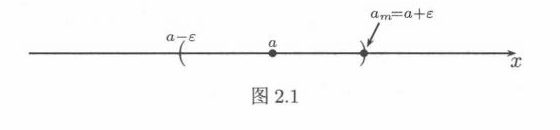
\includegraphics[width=.62\linewidth]{figures/upper/ch02/fig-2-1.png}
\end{center}

令 $M=\max\{a_1,a_2,\cdots,a_N\}$，则在 $n>N$ 时，有
\[
  a_n<a+\varepsilon=a+(a_m-a)=a_m\le M,
\]
可见 $M$ 是数列 $\{a_n\}$ 的最大数。同样可证在 $a_m<a$ 时，数列 $\{a_n\}$ 有最小数。

很容易举出不同时存在最大数和最小数的收敛数列的例子。例如数列 $\left\{\dfrac1n\right\}$ 收敛于 $0$，它有最大数，但没有最小数。

\textbf{证 2}\quad 若 $\{a_n\}$ 不是常值数列，则可从数列中取出不等的两项，设为 $a_s<a_t$，然后用反证法如下。设数列中既无最小数又无最大数，则存在无穷多项小于 $a_s$，又存在无穷多项大于 $a_t$。因此，所有大于 $a_s$ 或小于 $a_t$ 的实数都不可能是数列 $\{a_n\}$ 的极限。于是 $\{a_n\}$ 没有极限，与其收敛性矛盾。
\end{xproof}

下面一个例题有很多解法，这里举出两种不同解法。

\begin{xexample}[2.2.2]
若 $\displaystyle\lim_{n\to\infty}\frac{x_n-a}{x_n+a}=0$，证明 $\displaystyle\lim_{n\to\infty}x_n=a$。
\end{xexample}
\begin{xproof}
\textbf{证 1}\quad 由题设可见 $a\ne0$。由条件可知，$\forall\varepsilon>0,\exists N$，当 $n>N$ 时，成立
\[
  \abs{\frac{x_n-a}{x_n+a}}<\varepsilon.
\]
由此可估计出
\[
  \abs{x_n-a}<\varepsilon\abs{x_n+a}
  =\varepsilon\abs{(x_n-a)+2a}
  \le\varepsilon(\abs{x_n-a}+2\abs a).
\]
若限制 $\varepsilon<1$，则可得出 $\abs{x_n-a}<2\varepsilon\abs a/(1-\varepsilon)$。又若限制 $\varepsilon<1/2$，则又可得到
\[
  \abs{x_n-a}<\frac{2\varepsilon\abs a}{1-\varepsilon}<4\abs a\varepsilon.
\]
由于上式右边是 $\varepsilon$ 乘固定常数，可见成立 $\displaystyle\lim_{n\to\infty}x_n=a$。

\textbf{证 2}\quad 作代换
\[
  y_n=\frac{x_n-a}{x_n+a},
\]
则从 $a\ne0$ 可以看出对每个 $n$ 都有 $y_n\ne1$，因此就可以将 $x_n$ 用 $y_n$ 表示出来：
\[
  x_n=a\cdot\frac{1+y_n}{1-y_n},
\]
然后根据 $\displaystyle\lim_{n\to\infty}y_n=0$ 和极限运算法则就得到 $\displaystyle\lim_{n\to\infty}x_n=a$。
\end{xproof}

\begin{xremark}
\textbf{注 1}\quad 与适当放大法的例题不同，那里只是从数列收敛的定义出发，但在这两个证明中我们已经用到了收敛数列的许多基本知识。初学者要看到这个变化。

\textbf{注 2}\quad 在证 2 中用了变量代换法。这值得注意。实际上，若要证明 $\displaystyle\lim_{n\to\infty}x_n=a$，就可以令 $y_n=x_n-a$，然后去证明 $\displaystyle\lim_{n\to\infty}y_n=0$。这就是变量代换的最简单例子。应当指出，即使是如此平凡的代换，对于考虑问题也是有帮助的。
\end{xremark}

如何证明数列收敛和计算收敛数列的极限是这一章中的主要问题。一般说来，除了少数情况外，对于给定的一个数列 $\{a_n\}$，即使它是收敛的，我们也不知道它的极限是什么。这时在数列收敛定义中的 $a$ 不是一个已知量，不可能用来验证数列 $\{a_n\}$ 收敛。因此当然需要新的工具。

在研究数列收敛方面有两个工具是很基本的，这就是
\begin{itemize}
  \item 夹逼定理（也称为两面夹定理等）；
  \item 单调有界数列的收敛定理。
\end{itemize}
其中单调有界数列的收敛定理在理论上和应用上都非常重要，是本章的重点学习内容，我们将在下面 §2.3 中专门讨论。

夹逼定理是求极限的有力工具。其中包含的思想是，对难以直接处理的数列表达式，寻找两个较为简单的数列从两边夹住。如果这两个数列收敛于同一极限，则问题就解决了。能否找到这样两个数列是成功应用夹逼定理的关键。

下面是一个有代表性的例子，且有许多推广（参见例题 10.2.5）。

\begin{xexample}[2.2.3]
设 $a>0,b>0$，求极限 $\displaystyle\lim_{n\to\infty}(a^n+b^n)^{1/n}$。
\end{xexample}
\begin{xsolution}
不妨先假定 $a\le b$。这时就有两面夹的不等式：
\[
  b=(b^n)^{1/n}<(a^n+b^n)^{1/n}\le(2b^n)^{1/n},
\]
也就是 $b<(a^n+b^n)^{1/n}\le\sqrt[n]2\,b$。利用 $\displaystyle\lim_{n\to\infty}\sqrt[n]2=1$ 和夹逼定理，可见极限为 $b$。对 $a>b$ 可作类似讨论。最后的答案是 $\max\{a,b\}$。
\end{xsolution}

\begin{xexample}[2.2.4]
求数列 $\{a_n\}$ 的极限，其中
\[
  a_n=\frac{1!+2!+\cdots+n!}{n!},\qquad n\in\NN_+.
\]
\end{xexample}
\begin{xsolution}
将分子（设 $n>2$）中的前 $n-2$ 项适当放大，就有估计
\[
  1!+2!+\cdots+n!\le(n-2)(n-2)!+(n-1)!+n!<2(n-1)!+n!,
\]
因此知道在 $n>2$ 时，有
\[
  1<\frac{1!+2!+\cdots+n!}{n!}<\frac2n+1,
\]
令 $n\to\infty$ 即可知极限为 $1$。
\end{xsolution}

\subsection{判定数列发散的方法}

这里的基本方法有
\begin{enumerate}[label=\arabic*.]
  \item 无界数列一定发散。
  \item 从数列收敛的定义出发，用对偶法则就可得到（参考 §1.4）
  \[
    \{a_n\}\text{ 发散}\Longleftrightarrow
    \forall a,\exists\varepsilon_0>0,\forall N,\exists n>N,
    \text{ 使得 }\abs{a_n-a}\ge\varepsilon_0.
  \]
  \item 有一个发散子列的数列一定发散。
  \item 如果发现有两个子列不可能收敛于相同极限，则这个数列一定发散。
  \item Cauchy 收敛准则也是判定数列发散的充分必要条件（见下一章 §3.4）。
\end{enumerate}

在下面的例题中不但证明所给定的数列无界，而且证明它是正无穷大量。

\begin{xexample}[2.2.5]
根据无穷大量的定义证明
\[
  \lim_{n\to\infty}\frac{n^3+n-7}{n+3}=+\infty.
\]
\end{xexample}
\begin{xproof}
要对每个给定的 $G>0$，证明有 $N$，当 $n>N$ 时，有 $(n^3+n-7)/(n+3)>G$。不妨令 $n>3$，这样分母就可用 $2n$ 代替而使分式变小。由于这时分子中的 $n^3-7>\frac12n^3$，又去掉分子中的 $n$，这样就可以估计出
\[
  \frac{n^3+n-7}{n+3}>\frac{\frac12n^3}{2n}=\frac14n^2>\frac14n.
\]
为使最后一式大于 $G$，只要取 $N=\max\{3,[4G]\}$ 即可。
\end{xproof}

\begin{xremark}
这里所用的方法与前面的“适当放大法”完全一样，但或许应称为“适当缩小法”了。容易看出，本题的关键在于分子的最高次数高于分母的最高次数。只要保持这一特点，在简化时就可以慷慨地缩小，最后得到 $N$ 的简单表达式。
\end{xremark}

接下来的例题是数学分析中的一个重要结果，这里将给出 3 个证明，并在几个注解中作进一步的补充。

\begin{xexample}[2.2.6]
设
\[
  S_n=1+\frac12+\frac13+\cdots+\frac1n,\qquad n\in\NN_+,
\]
证明数列 $\{S_n\}$ 发散。
\end{xexample}

数列 $\{S_n\}$ 发散是不容易猜出来的。如果读者（用计算器或计算机）试算一下这个数列的前若干项，就会发现这个数列增长得很慢。从第一项 $S_1=1$ 开始，到 $S_{83}$ 才第一次大于 5，到 $S_{12367}$ 才刚超过 10。今后在 2.5.3 小节中学了有关 Euler 常数的知识后我们就能够准确估计 $S_n$ 的近似值。这里的精彩故事见数学通俗读物 [12] 的第八章。

历史上的证明最早是 Oresme（奥雷姆，约 1323—1382）在 1360 年左右发表的（见 [29]）。后来 Bernoulli 兄弟，Jacob Bernoulli（1655—1705）和 Johann Bernoulli（1667—1748），在 1689 年左右又给出了两个证明。

\begin{xproof}
\textbf{证 1}\quad 较为常见的证明就是 Oresme 的方法，其实质是利用不等式
\begin{equation}
  \frac1{n+1}+\frac1{n+2}+\cdots+\frac1{2n}>n\cdot\frac1{2n}=\frac12.
  \tag{2.3}
  \label{eq:2.3}
\end{equation}
这样就可以得到
\[
  S_2=1+\frac12,
  \qquad
  S_4=S_2+\frac13+\frac14>S_2+2\left(\frac14\right)=2,
\]
\[
  S_8=S_4+\frac15+\frac16+\frac17+\frac18
  >S_4+4\left(\frac18\right)>1+\frac32=2.5,
\]
$\cdots\cdots$。

不难用数学归纳法证明（请读者完成）：对每一个 $n$，成立不等式
\[
  S_{2^n}\ge1+\frac n2.
\]
可见数列 $\{S_n\}$ 无上界，因此发散。

\textbf{证 2}\quad 这是 Jacob Bernoulli 的证明（引自 [29]）。他发现对任意的正整数 $n$，有
\[
  \frac1{n+1}+\frac1{n+2}+\cdots+\frac1{n^2}>\frac{n^2-n}{n^2}=1-\frac1n,
\]
因此得到不等式
\begin{equation}
  \frac1n+\frac1{n+1}+\cdots+\frac1{n^2}>1.
  \tag{2.4}
  \label{eq:2.4}
\end{equation}
由于 $n$ 是任意的，这样就知道
\[
  S_4=1+\frac12+\frac13+\frac14>2,
\]
\[
  S_{25}=S_4+\frac15+\cdots+\frac1{25}>3,
\]
依此类推，可见数列 $\{S_n\}$ 不可能收敛。

\textbf{证 3}\quad 用反证法：若 $\{S_n\}$ 收敛，记 $S=\displaystyle\lim_{n\to\infty}S_n$。分析 $S_{2n}=A_n+B_n$，其中
\[
  A_n=1+\frac13+\frac15+\cdots+\frac1{2n-1},
  \qquad
  B_n=\frac12+\frac14+\frac16+\cdots+\frac1{2n}.
\]
由于 $B_n=\frac12S_n$，因此 $\displaystyle\lim_{n\to\infty}B_n=\frac12S$。但由此又可以计算出
\[
  \lim_{n\to\infty}A_n
  =\lim_{n\to\infty}(S_{2n}-B_n)=\frac12S.
\]
比较 $A_n$ 和 $B_n$，对每个 $n$ 都有 $A_n-B_n>\frac12$，因此 $\{A_n\}$ 和 $\{B_n\}$ 收敛于同一个极限值是不可能的。
\end{xproof}

\begin{xremark}
由于 $\{S_n\}$ 是严格单调增加数列。在前两个证明的基础上不难证明 $\{S_n\}$ 是正无穷大量。此外，例题 2.2.6 还有许多其他解法。在例题 2.3.4 中将会证明数列
\[
  \left\{\frac1{n+1}+\cdots+\frac1{2n}\right\}
\]
收敛，而且极限大于 0。由于这个数列的通项就是 $S_{2n}-S_n$，如果数列 $\{S_n\}$ 收敛，则 $\displaystyle\lim_{n\to\infty}(S_{2n}-S_n)=0$。这与例题 2.3.4 的结论矛盾，可看成是本题的第 4 个证明。在例题 3.4.2 中用 Cauchy 收敛准则又对本题给出新证明。
\end{xremark}

下一个例题将介绍如何用构造两个子列的方法来证明数列发散。

\begin{xexample}[2.2.7]
证明数列 $\{\sin n\}$ 发散。
\end{xexample}
\begin{xproof}
\textbf{证 1（几何方法）}\quad 从正弦曲线 $y=\sin x$ 的图像（如图 2.2）可以设法构造出两个子列。虽然我们并不知道它们是否收敛，但却有把握知道它们（如果收敛的话）决不可能收敛于同一极限。现在观察 $y=\sin x$ 在一个周期上的几何图像：

\begin{center}
  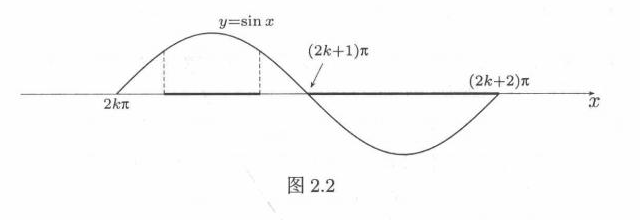
\includegraphics[width=.66\linewidth]{figures/upper/ch02/fig-2-2.png}
\end{center}

先看图 2.2 中介于 $2k\pi$ 和 $(2k+1)\pi$ 之间的（加黑的）区间 $[2k\pi+(\pi/4),2k\pi+(3\pi/4)]$。由于函数 $\sin x$ 在这个区间上的取值不小于 $\sin(\pi/4)=\sqrt2/2$，同时区间长度又大于 1，因此在该区间中一定存在一个正整数，记为 $n_k'$。对每个 $k$ 都这样做，就得到一个子列 $\{\sin n_k'\}$。如果它收敛的话，其极限一定不小于 $\sqrt2/2$。

类似地可以在图 2.2 上的区间 $[(2k+1)\pi,(2k+2)\pi]$ 中选出正整数 $n_k''$，得到第二个子列 $\{\sin n_k''\}$。它如果收敛的话，极限一定不会大于 0。

因为收敛数列的每个子列都收敛于同一极限，而现在所构造出的两个子列即使都收敛，也不可能收敛于同一极限，从而就推知 $\{\sin n\}$ 是发散数列。

利用正弦函数的特殊性，本题也可以证明如下。

\textbf{证 2}\quad 用反证法。设存在 $\displaystyle\lim_{n\to\infty}\sin n=a$，则就有 $\sin(n+1)-\sin(n-1)\to0$。由于
\[
  \sin(n+1)-\sin(n-1)=2\sin1\cos n,
\]
因此得到 $\cos n\to0$。再利用
\[
  \cos(n+1)-\cos(n-1)=-2\sin n\sin1\to0,
\]
又得到 $\sin n\to0$。这样就有
\[
  \lim_{n\to\infty}\sin n=\lim_{n\to\infty}\cos n=0.
\]
这与恒等式 $\sin^2n+\cos^2n=1$ 相矛盾。
\end{xproof}

\begin{xremark}
本例题的解法还有很多，见下一章的例题 3.4.3。
\end{xremark}

下一个例题的方法与上面完全不同。在 §2.6 将对这类“迭代”数列作专题讨论。

\begin{xexample}[2.2.8]
设 $x_1=\dfrac c2$，$x_{n+1}=\dfrac c2+\dfrac{x_n^2}{2}$，$n\in\NN_+$，证明：若 $c>1$，则 $\{x_n\}$ 发散。
\end{xexample}
\begin{xproof}
用反证法。若数列 $\{x_n\}$ 收敛，记其极限为 $A$。在递推公式
\[
  x_{n+1}=\frac c2+\frac{x_n^2}{2}
\]
两边令 $n\to\infty$，就得到
\[
  A=\frac c2+\frac{A^2}{2}.
\]
这表明极限值 $A$ 应当满足二次方程 $A^2-2A+c=0$。但由于这个二次方程的判别式 $\Delta=4-4c<0$，因此无实根，这表明 $A$ 不存在，因此数列 $\{x_n\}$ 发散。
\end{xproof}

\begin{xremark}
\textbf{注 1}\quad 显然，$\{x_n\}$ 在 $c>0$ 时严格单调增加，因此在 $c>1$ 时是正无穷大量。

\textbf{注 2}\quad 这个例题是 [14] 的第一卷的第 35 小节中例 6 的一部分。在那里对参数 $c$ 的其他情况作了详细研究。但其中对于 $c<-3$ 时未作深入讨论就说数列 $\{x_n\}$ 发散，这是不正确的。在 [24] 的 8—14 页对此题作了完整的讨论，其中证明存在可列个参数值 $c<-3$ 使得 $\{x_n\}$ 收敛。由于此题的迭代方程在 $c<1$ 时通过线性变换 $x=(1+\sqrt{1-c})(1-2y)$ 即可成为本章第二组参考题 19（以及 2.6.3 小节中的题 3）中的 logistic（逻辑斯谛）映射（抛物线映射）的迭代系统，因此本书正文中不再讨论 $c\le1$ 的情况。
\end{xremark}

下一个例题的内容和证明都很简单，但实际上是无穷级数收敛的一个必要条件。这在无穷级数理论中是一个基本内容。

\begin{xexample}[2.2.9]
设有两个数列 $\{S_n\}$ 和 $\{a_n\}$，且有关系如下：
\[
  S_n=a_1+a_2+\cdots+a_n,\qquad n\in\NN_+.
\]
若 $\{S_n\}$ 收敛，则 $\{a_n\}$ 为无穷小量。反之，若 $\{a_n\}$ 不是无穷小量，则 $\{S_n\}$ 发散。
\end{xexample}
\begin{xproof}
从 $n\ge2$ 起有 $a_n=S_n-S_{n-1}$，又当 $\{S_n\}$ 收敛时，$\{S_{n-1}\}_{n\ge2}$ 也一定收敛，而且收敛于同一极限，在上式两边取 $n\to\infty$，就得到 $\displaystyle\lim_{n\to\infty}a_n=0$。
\end{xproof}

\begin{xremark}
对于给定的数列 $\{a_n\}$，将记号
\[
  \sum_{n=1}^{\infty}a_n=a_1+a_2+\cdots+a_n+\cdots
\]
称为以 $a_n$ 为通项的无穷级数。从 $\{a_n\}$ 出发，就可以如例题 2.2.9 中的关系式那样定义数列 $\{S_n\}$，称为该无穷级数的部分和数列，如果 $\{S_n\}$ 收敛，并有
\[
  \lim_{n\to\infty}S_n=S,
\]
则定义该无穷级数收敛，且称 $S$ 为该无穷级数的和，记为
\[
  \sum_{n=1}^{\infty}a_n=a_1+a_2+\cdots+a_n+\cdots=S.
\]
否则就说该无穷级数发散。

无穷级数理论具有极其丰富的内容，是本书下册的中心内容之一。但由以上的简单介绍也已经可以看出，无穷级数与数列有密切的联系。实际上前面的例题 2.2.6 的内容就是证明以 $1/n$ 为通项的无穷级数发散（于正无穷大）。这个级数一般称为调和级数。

用无穷级数的语言来说，例题 2.2.9 的内容是：无穷级数收敛的必要条件是它的通项（所成的数列）收敛于 0。当然，这并非是充分条件，用例题 2.2.6 就可以说明这一点。
\end{xremark}

\subsection{练习题}

\begin{xexercise}[1]
证明：$\{a_n\}$ 收敛的充分必要条件是 $\{a_{2k}\}$ 和 $\{a_{2k-1}\}$ 收敛于同一极限。
\end{xexercise}
\begin{xsolution}
必要性显然，因为收敛数列的任一子列都收敛于原极限。

反之，设
\[
  a_{2k}\to A,\qquad a_{2k-1}\to A.
\]
给定 $\varepsilon>0$，分别取 $K_1,K_2$，使 $k>K_1$ 时 $\abs{a_{2k}-A}<\varepsilon$，$k>K_2$ 时 $\abs{a_{2k-1}-A}<\varepsilon$。取 $N>2\max\{K_1,K_2\}+1$，则任意 $n>N$ 无论奇偶都满足 $\abs{a_n-A}<\varepsilon$，故 $a_n\to A$。
\end{xsolution}


\begin{xexercise}[2]
以下是可以应用夹逼定理的几个题：
  \begin{enumerate}[label=(\arabic*)]
    \item 给定 $p$ 个正数 $a_1,a_2,\cdots,a_p$，求 $\displaystyle\lim_{n\to\infty}\sqrt[n]{a_1^n+a_2^n+\cdots+a_p^n}$；
    \item 设 $x_n=\dfrac1{\sqrt{n^2+1}}+\dfrac1{\sqrt{n^2+2}}+\cdots+\dfrac1{\sqrt{(n+1)^2}}$，$n\in\NN_+$，求 $\displaystyle\lim_{n\to\infty}x_n$；
    \item 设 $a_n=\left(1+\dfrac12+\cdots+\dfrac1n\right)^{1/n}$，$n\in\NN_+$，求 $\displaystyle\lim_{n\to\infty}a_n$；
    \item 设 $\{a_n\}$ 为正数列，并且已知它收敛于 $a>0$，证明 $\displaystyle\lim_{n\to\infty}\sqrt[n]{a_n}=1$。
  \end{enumerate}
\end{xexercise}
\begin{xsolution}
(1) 令 $M=\max\{a_1,\ldots,a_p\}$。则
\[
  M^n\le a_1^n+\cdots+a_p^n\le pM^n.
\]
开 $n$ 次方得到
\[
  M\le\sqrt[n]{a_1^n+\cdots+a_p^n}\le p^{1/n}M\to M.
\]
故极限为 $M$。

(2) 和式共有 $2n+1$ 项，并且
\[
  \frac{2n+1}{n+1}
  \le x_n
  \le\frac{2n+1}{\sqrt{n^2+1}}.
\]
两端都趋于 $2$，故 $x_n\to2$。

(3) 记 $H_n=1+1/2+\cdots+1/n$。显然
\[
  1\le H_n\le n,
\]
所以
\[
  1\le H_n^{1/n}\le n^{1/n}\to1.
\]
故极限为 $1$。

(4) 因 $a_n\to a>0$，充分大的 $n$ 有
\[
  \frac a2<a_n<\frac{3a}{2}.
\]
于是
\[
  \left(\frac a2\right)^{1/n}
  <a_n^{1/n}
  <\left(\frac{3a}{2}\right)^{1/n}.
\]
两端均趋于 $1$，由夹逼定理得 $a_n^{1/n}\to1$。
\end{xsolution}


\begin{xexercise}[3]
求下列极限：
  \begin{enumerate}[label=(\arabic*)]
    \item $\displaystyle\lim_{n\to\infty}(1+x)(1+x^2)\cdots(1+x^{2^n})$，其中 $\abs{x}<1$；
    \item $\displaystyle\lim_{n\to\infty}\left(1-\frac1{2^2}\right)\left(1-\frac1{3^2}\right)\cdots\left(1-\frac1{n^2}\right)$；
    \item $\displaystyle\lim_{n\to\infty}\left(1-\frac1{1+2}\right)\left(1-\frac1{1+2+3}\right)\cdots\left(1-\frac1{1+2+\cdots+n}\right)$；
    \item $\displaystyle\lim_{n\to\infty}\left[\frac1{1\cdot2\cdot3}+\frac1{2\cdot3\cdot4}+\cdots+\frac1{n(n+1)(n+2)}\right]$；
    \item $\displaystyle\lim_{n\to\infty}\sum_{k=1}^n\frac1{k(k+1)\cdots(k+\nu)}$（其中 $\nu$ 为正整数）。
  \end{enumerate}
  （最后两个题是 $\displaystyle\lim_{n\to\infty}\left[\frac1{1\cdot2}+\frac1{2\cdot3}+\cdots+\frac1{n(n+1)}\right]$ 的推广。）
\end{xexercise}
\begin{xsolution}
(1) 利用恒等式
\[
  (1-x)\prod_{j=0}^n(1+x^{2^j})=1-x^{2^{n+1}},
\]
可得当 $\abs x<1$ 时
\[
  \prod_{j=0}^n(1+x^{2^j})	o\frac1{1-x}.
\]

(2)
\[
  \prod_{k=2}^n\left(1-\frac1{k^2}\right)
  =\prod_{k=2}^n\frac{k-1}{k}\frac{k+1}{k}
  =\frac{n+1}{2n}\to\frac12.
\]

(3) 因 $1+2+\cdots+k=k(k+1)/2$，
\[
  1-\frac1{1+\cdots+k}
  =1-\frac2{k(k+1)}
  =\frac{k-1}{k}\frac{k+2}{k+1}.
\]
从 $k=2$ 到 $n$ 连乘得
\[
  \frac1n\cdot\frac{n+2}{3}=\frac{n+2}{3n}\to\frac13.
\]

(4) 分解
\[
  \frac1{k(k+1)(k+2)}
  =\frac12\left(\frac1{k(k+1)}-\frac1{(k+1)(k+2)}\right).
\]
故前 $n$ 项和为
\[
  \frac14-\frac1{2(n+1)(n+2)}\to\frac14.
\]

(5) 对正整数 $\nu$，
\[
  \frac1{k(k+1)\cdots(k+\nu)}
  =\frac1\nu\left[
    \frac1{k(k+1)\cdots(k+\nu-1)}
    -\frac1{(k+1)\cdots(k+\nu)}
  \right].
\]
于是望远镜相消后
\[
  \sum_{k=1}^n\frac1{k(k+1)\cdots(k+\nu)}
  =\frac1\nu\left(\frac1{\nu!}-\frac1{(n+1)\cdots(n+\nu)}\right),
\]
极限为
\[
  \boxed{\frac1{\nu\,\nu!}}.
\]
\end{xsolution}


\begin{xexercise}[4]
设 $s_n=a+3a^2+\cdots+(2n-1)a^n$，$\abs a<1$，求 $\{s_n\}$ 的极限。

  （试计算 $s_n-as_n$。）
\end{xexercise}
\begin{xsolution}
按题目提示计算 $s_n-as_n$。有
\begin{align*}
  (1-a)s_n
  &=a+2(a^2+a^3+\cdots+a^n)-(2n-1)a^{n+1}\\
  &=a+\frac{2a^2(1-a^{n-1})}{1-a}-(2n-1)a^{n+1}.
\end{align*}
因 $\abs a<1$，有 $a^n\to0$ 且 $na^n\to0$，故令 $n\to\infty$ 得
\[
  (1-a)\lim_{n\to\infty}s_n
  =a+\frac{2a^2}{1-a}
  =\frac{a(1+a)}{1-a}.
\]
因此
\[
  \boxed{\lim_{n\to\infty}s_n=\frac{a(1+a)}{(1-a)^2}}.
\]
\end{xsolution}


\begin{xexercise}[5]
设正数列 $\{x_n\}$ 收敛，极限大于 0，证明：这个数列有正下界，但在数列中不一定有最小数。
\end{xexercise}
\begin{xsolution}
设 $x_n\to L>0$。取 $N$ 使 $n>N$ 时 $x_n>L/2$。再令
\[
  m=\min\{x_1,\ldots,x_N,L/2\}>0,
\]
则对所有 $n$ 都有 $x_n\ge m$，故有正下界。

但最小数不一定存在。例如 $x_n=1+1/n$ 收敛于 $1>0$，以 $1$ 为正下界，却没有任何一项等于最小值 $1$。
\end{xsolution}


\begin{xexercise}[6]
证明：若有 $\displaystyle\lim_{n\to\infty}a_n=+\infty$，则在数列 $\{a_n\}$ 中一定有最小数。
\end{xexercise}
\begin{xsolution}
由 $a_n\to+\infty$，取 $G=a_1$，存在 $N$ 使 $n>N$ 时 $a_n>a_1$。有限集合 $\{a_1,\ldots,a_N\}$ 有最小值 $m$，而所有尾项又都大于 $a_1\ge m$，所以 $m$ 就是整个数列的最小数。
\end{xsolution}


\begin{xexercise}[7]
证明：无界数列至少有一个子列是确定符号的无穷大量。
\end{xexercise}
\begin{xsolution}
无界意味着至少有一侧无界：或者数列没有上界，或者没有下界。

若没有上界，递归选取 $n_k>n_{k-1}$ 使 $a_{n_k}>k$，则 $a_{n_k}\to+\infty$。若没有下界，则可选 $n_k$ 使 $a_{n_k}<-k$，于是 $a_{n_k}\to-\infty$。因此至少存在一个确定符号的无穷大量子列。
\end{xsolution}


\begin{xexercise}[8]
证明数列 $\{\tan n\}$ 发散。
\end{xexercise}
\begin{xsolution}
用反证法。若 $\tan n\to L$，则移位数列也趋于 $L$，故 $\tan(n+1)-\tan n\to0$。由正切加法公式
\[
  \tan(n+1)=\frac{\tan n+\tan1}{1-\tan n\tan1}.
\]
若 $1-L\tan1\ne0$，令 $n\to\infty$ 得
\[
  L=\frac{L+\tan1}{1-L\tan1},
\]
即 $\tan1(1+L^2)=0$，不可能。若 $1-L\tan1=0$，右端分母趋于 $0$ 而分子趋于 $L+\tan1\ne0$，也不可能收敛到有限的 $L$。故 $\{\tan n\}$ 发散。
\end{xsolution}


\begin{xexercise}[9]
设数列 $\{S_n\}$ 的定义为
  \[
    S_n=1+\frac1{2^p}+\frac1{3^p}+\cdots+\frac1{n^p},\qquad n\in\NN_+.
  \]
  证明 $\{S_n\}$ 在以下两种情况均发散：(1) $p\le0$，(2) $0<p<1$。
\end{xexercise}
\begin{xsolution}
若 $p\le0$，则 $k^{-p}\ge1$，所以 $S_n\ge n\to+\infty$。

若 $0<p<1$，取 $n\ge2$。从 $k=\lceil n/2\rceil$ 到 $n$ 至少有 $n/2$ 项，且每项不小于 $1/n^p$，故
\[
  S_n\ge\frac n2\cdot\frac1{n^p}
  =\frac12n^{1-p}\to+\infty.
\]
两种情形均发散，而且实际上都趋于 $+\infty$。
\end{xsolution}


\section{单调数列}

关于单调数列的基本结论很简单，只不过是
\begin{enumerate}[label=(\arabic*)]
  \item 单调有界数列一定收敛；
  \item 单调无界数列一定是有确定符号的无穷大量。
\end{enumerate}
然而这两个基本结论在数列的研究中起着很重要的作用。它们不仅是本节各个例题中的主要工具，而且也是学习 §2.5 和 §2.6 的基础。

与 §2.1 一开始的收敛数列的定义相比较，可以看出对单调数列来说，我们可以从数列本身判定其收敛或发散，而不需要对极限的存在或不存在作假定。这是一个很大的进步。由于对单调有界数列只肯定了它的极限存在，而没有给出极限本身，因此这是在数学中的存在性定理的一个典型例子。从下面的例题可以看出，极限的存在性有时能帮助我们将极限计算出来。

如何对一般的数列从其本身来判定它收敛还是发散？这就是下一章 §3.4 中的 Cauchy 收敛准则要回答的问题。

\subsection{例题}

收敛数列当然不一定是单调数列，但是有很多常用的数列确实是单调的，或者从某一项开始是单调的。例如以下几个常见数列的收敛性都可以从单调性出发得到证明（虽然不一定是最佳的证明方法），并求出它们的极限：
\[
  \{\sqrt[n]{a}\}\ (a>0),\quad
  \{\sqrt[n]{n}\},\quad
  \left\{\frac{n^k}{a^n}\right\}\ (k>0,a>1),\quad
  \left\{\frac{a^n}{n!}\right\},\quad
  \left\{\frac{n!}{n^n}\right\}.
\]

为了知道一个数列是否单调，一个自然的方法就是去比较数列中相继两项的大小。这可以通过分析相继两项之比或之差来达到目的。以下几个例子都是如此，其中还介绍在知道极限存在后如何计算极限。

下面的前两个例题是上一节的例题 2.1.1 和 2.1.2 的新解，但在问题的提法上有不同，不再是验证已给定数列是否以某个数为其极限了。

\begin{xexample}[2.3.1]
用单调有界数列的收敛定理，证明 $\left\{\dfrac{n^5}{2^n}\right\}$ 收敛，并求其极限。
\end{xexample}
\begin{xproof}
记数列的通项为 $a_n=\dfrac{n^5}{2^n}$，$n\in\NN_+$，则可以看出前后两项之比为
\[
  \frac{a_{n+1}}{a_n}=\frac12\left(1+\frac1n\right)^5.
\]
分析上式右边的第二个因子，从 $\displaystyle\lim_{n\to\infty}\left(1+\frac1n\right)^5=1$，可见存在 $N$，当 $n>N$ 时，满足不等式 $\left(1+\dfrac1n\right)^5<2$。因此，当 $n>N$ 时，就有
\begin{equation}
  a_{n+1}=a_n\cdot\frac12\left(1+\frac1n\right)^5<a_n.
  \tag{2.5}
  \label{eq:2.5}
\end{equation}
由此可见，至少从 $n>N$ 起数列 $\{a_n\}$ 严格单调减少。又由于 $\{a_n\}$ 是正数列，以 0 为下界，因此就可以用单调有界数列的收敛定理，知道存在极限 $a=\displaystyle\lim_{n\to\infty}a_n$。利用极限的存在性，在 (2.5) 左边的等式两边令 $n\to\infty$，就有
\[
  a=\frac12a\Longrightarrow a=0.
\]
\end{xproof}

\begin{xremark}
希望初学者比较这个方法与例题 2.1.1 中的方法。这里在问题的提法、采取的思路和所需要的工具等方面都完全不同。
\end{xremark}

\begin{xexample}[2.3.2]
研究数列 $\{\sqrt[n]{n}\}$ 是否单调，并求出该数列的极限。
\end{xexample}
\begin{xproof}
记 $a_n=\sqrt[n]{n}$，$n\in\NN_+$。计算数列的前几项，得 $a_1=1,a_2=\sqrt2$，以及 $a_3=\sqrt[3]3\approx1.44,a_4=a_2\approx1.41,a_5=\sqrt[5]5\approx1.38,a_6=\sqrt[6]6\approx1.35,\cdots$，可见这个数列有可能从第三项起严格单调减少。比较前后两项，由于有
\[
  a_{n+1}=\sqrt[n+1]{n+1}<a_n=\sqrt[n]n
  \Longleftrightarrow
  \left(1+\frac1n\right)^n<n,
\]
只要证明当 $n$ 充分大时右边的不等式成立，就可以证实我们的猜测正确。利用平均值不等式，可以得到
\[
  \frac1n\left(1+\frac1n\right)^n
  =\left(\frac1{\sqrt n}\right)^2\left(1+\frac1n\right)^n
  <\left(\frac{n+1+2/\sqrt n}{n+2}\right)^{n+2},
\]
可见只要 $n>4$ 就可以使上式右边的表达式严格小于 1。因此数列 $\{\sqrt[n]n\}$ 至少从第 5 项起是严格单调减少数列。又由于这个数列以 1 为下界，因此从单调有界数列的收敛定理知道，存在极限
\[
  \lim_{n\to\infty}\sqrt[n]n=a\ge1.
\]
以下只要证明 $a>1$ 是不可能的。用反证法。若有 $a=1+h,h>0$，则当 $n$ 充分大时应当成立 $\sqrt[n]n>1+h$，从而得到
\[
  n>(1+h)^n>\frac{n(n-1)}2h^2.
\]
但这是不可能的。因此得出结论：$\displaystyle\lim_{n\to\infty}\sqrt[n]n=1$。
\end{xproof}

对数列研究前后两项之比可以提升为一种方法，并建立如下结果。

\begin{xexample}[2.3.3]
设对于 $\{a_n\}$，有
\[
  \lim_{n\to\infty}\abs{\frac{a_{n+1}}{a_n}}=c<1,
\]
则 $\{a_n\}$ 是无穷小量。
\end{xexample}
\begin{xproof}
取 $\varepsilon=(1-c)/2$，有 $N$，当 $n>N$ 时，成立
\[
  \abs{\frac{a_{n+1}}{a_n}}<c+\frac{1-c}{2}=\frac{1+c}{2}<1,
\]
因此在 $n>N$ 时 $\{\abs{a_n}\}$ 是严格单调减少数列。由于它以 0 为下界，因此收敛。记它的极限为 $a$。在不等式
\begin{equation}
  \abs{a_{n+1}}<\frac{1+c}{2}\abs{a_n}
  \tag{2.6}
  \label{eq:2.6}
\end{equation}
两边令 $n\to\infty$，就得到 $0\le a\le a(1+c)/2$。因为 $0<(1+c)/2<1$，这只能导致 $a=0$。从 $\{\abs{a_n}\}$ 收敛于 0 可知 $\{a_n\}$ 也收敛于 0。
\end{xproof}

\begin{xremark}
这个例题中由于有很强的条件，不用单调有界数列的收敛定理也能证出来。例如，在得到不等式 (2.6) 后，引入记号 $c_1=(1+c)/2$，然后证明存在常数 $M>0$，使不等式 $\abs{a_n}<Mc_1^n$ 在 $n>N$ 时成立，由于 $c_1\in(0,1)$，可知有 $\displaystyle\lim_{n\to\infty}\abs{a_n}=0$。因此，对一般的数列研究其后项与前项之比也可能有用处。
\end{xremark}

\begin{xexample}[2.3.4]
设
\[
  a_n=\frac1{n+1}+\cdots+\frac1{2n},\qquad n\in\NN_+,
\]
证明数列 $\{a_n\}$ 收敛。
\end{xexample}
\begin{xproof}
比较数列的前后两项之差，就可发现
\[
  a_{n+1}-a_n=\frac1{2n+1}+\frac1{2n+2}-\frac1{n+1}
  >2\cdot\frac1{2n+2}-\frac1{n+1}=0,
\]
可见数列单调增加。由于 $a_n<\dfrac n{n+1}<1$，可取 1 作为上界，因此数列收敛。
\end{xproof}

\begin{xremark}
以后将会求出本题中的数列极限是 $\ln2$（见例题 2.5.4，11.4.1）。
\end{xremark}

下一个例子并不难，但是其中的方法很基本，同时它的结论自 1976 年后在计算数学中变得很有用（见例题后的注解）。

\begin{xexample}[2.3.5]
给定两个正数 $a$ 和 $b$，且有 $0<b<a$。令 $a_0=a,b_0=b$，并按照递推公式
\[
  a_n=\frac{a_{n-1}+b_{n-1}}2,
  \qquad
  b_n=\sqrt{a_{n-1}b_{n-1}},
  \qquad n\in\NN_+,
\]
定义数列 $\{a_n\}$ 和 $\{b_n\}$。证明这两个数列收敛于同一个极限。
\end{xexample}
\begin{xproof}
利用 $0<b_0<a_0$ 和平均值不等式，可以得到 $b_0<b_1<a_1<a_0$。用数学归纳法可以证明对每个 $n$ 均成立
\[
  b_0<b_1<\cdots<b_n<a_n<\cdots<a_1<a_0.
\]
因此数列 $\{a_n\}$ 和 $\{b_n\}$ 都是单调有界的，记极限为 $A$ 和 $B$，则均为正数。在两个迭代式中任取一个，令 $n\to\infty$，就得到 $A=B$。
\end{xproof}

\begin{xremark}
一般称上述极限为数 $a$ 和 $b$ 的算术几何平均值，记为 $AG(a,b)$。利用积分换元计算可以得到 $AG(a,b)$ 的解析表达式（见 [14] 第二卷的 315 小节）：
\[
  AG(a,b)=\frac{\pi}{2G},\qquad
  \text{其中 }G=\int_0^{\pi/2}\frac{\dd x}{\sqrt{a^2\cos^2x+b^2\sin^2x}}.
\]
算术几何平均值和上述解析表达式是大数学家 Gauss（高斯）在 14 岁（1791 年）时发现的，在他的早期研究工作中起了重要的作用。但这个结果长期以来没有引起足够重视，直到 1976 年才由 Salamin（萨拉明）和 Brent（布伦特）等人以此为基础发展出一种算术几何平均值快速算法，成为目前在计算机上计算圆周率 $\pi$ 和初等函数的最有效方法之一。例如对于 $\pi$ 来说，这种算法每计算一步可以使 $\pi$ 的有效位数增加一倍或更多（见例题 8.7.2 及其注之后的介绍）。关于 $\pi$ 在历年来的许多奇妙发现可以参看 [1, 60]。
\end{xremark}

下一题就是前面的例题 2.2.4，但方法与当时的夹逼方法完全不同。

\begin{xexample}[2.3.6]
求数列 $\{a_n\}$ 的极限，其中
\[
  a_n=\frac{1!+2!+\cdots+n!}{n!},\qquad n\in\NN_+.
\]
\end{xexample}
\begin{xsolution}
研究相继两项之比 $\dfrac{a_{n+1}}{a_n}$，有
\[
  \frac{a_{n+1}}{a_n}
  =\frac{1!+2!+\cdots+(n+1)!}{(n+1)(1!+2!+\cdots+n!)}
  =\frac{3+3!+\cdots+(n+1)!}{(n+1)+(n+1)2!+\cdots+(n+1)n!}.
\]
在 $n>2$ 时分母的每一项大于等于分子的对应项，因此 $\{a_n\}$ 在 $n>2$ 后单调减少。由于 0 是下界，因此数列收敛。又可发现联系前后两项的另一个关系式为
\[
  a_{n+1}=1+\frac{a_n}{n+1},
\]
在两边令 $n\to\infty$，即知极限为 1。
\end{xsolution}

\subsection{练习题}

\begin{xexercise}[1]
证明：若 $\{x_n\}$ 单调，则 $\{\abs{x_n}\}$ 至少从某项开始后单调。又问：反之如何？
\end{xexercise}
\begin{xsolution}
设 $x_n$ 单调增加。若它最终非负，则从那一项起 $\abs{x_n}=x_n$ 仍单调增加；若它始终为负，则 $\abs{x_n}=-x_n$ 单调减少；若由负变正，单调数列至多跨过 $0$ 一次，所以跨过后绝对值仍单调。单调减少的情形完全类似。因此 $\abs{x_n}$ 总会从某项起单调。

反之不成立。例如 $x_n=(-1)^n$，则 $\abs{x_n}\equiv1$ 是单调的常值数列，但 $x_n$ 本身不单调。
\end{xsolution}


\begin{xexercise}[2]
设 $\{a_n\}$ 单调增加，$\{b_n\}$ 单调减少，且有 $\displaystyle\lim_{n\to\infty}(a_n-b_n)=0$。证明：数列 $\{a_n\}$ 和 $\{b_n\}$ 都收敛，且极限相等。
\end{xexercise}
\begin{xsolution}
令 $d_n=a_n-b_n$。由于 $a_n$ 单调增加而 $b_n$ 单调减少，$d_n$ 单调增加；又 $d_n\to0$，所以对所有 $n$ 有 $d_n\le0$，即 $a_n\le b_n$。

于是
\[
  a_1\le a_n\le b_n\le b_1.
\]
$\{a_n\}$ 单调增加且有上界，$\{b_n\}$ 单调减少且有下界，故二者都收敛。设极限分别为 $A,B$，由 $a_n-b_n\to0$ 得 $A-B=0$，故 $A=B$。
\end{xsolution}


\begin{xexercise}[3]
按照极限的定义证明：单调增加有上界的数列的极限不小于数列的任何一项，单调减少有下界的数列的极限不大于数列的任何一项。
\end{xexercise}
\begin{xsolution}
设 $a_n$ 单调增加且 $a_n\to A$。固定任意 $k$，对所有 $n\ge k$ 有 $a_k\le a_n$。令 $n\to\infty$，由极限的保序性得 $a_k\le A$。因此极限不小于任一项。

若 $a_n$ 单调减少且趋于 $A$，同理对 $n\ge k$ 有 $a_k\ge a_n$，令 $n\to\infty$ 得 $a_k\ge A$，即极限不大于任一项。
\end{xsolution}


\begin{xexercise}[4]
设 $x_n=\dfrac23\cdot\dfrac35\cdots\dfrac{n+1}{2n+1}$，$n\in\NN_+$，求数列 $\{x_n\}$ 的极限。
\end{xexercise}
\begin{xsolution}
记
\[
  x_n=\frac23\frac35\cdots\frac{n+1}{2n+1}>0.
\]
则
\[
  \frac{x_{n+1}}{x_n}=\frac{n+2}{2n+3}\to\frac12<1.
\]
取 $q\in(1/2,1)$，充分大的 $n$ 有 $x_{n+1}<q x_n$，从而尾部被一个趋于 $0$ 的几何数列控制。故
\[
  \boxed{x_n\to0}.
\]
\end{xsolution}


\begin{xexercise}[5]
设 $a_n=\dfrac{10}{1}\cdot\dfrac{11}{3}\cdots\dfrac{n+9}{2n-1}$，$n\in\NN_+$，求数列 $\{a_n\}$ 的极限。
\end{xexercise}
\begin{xsolution}
记
\[
  a_n=\frac{10}{1}\frac{11}{3}\cdots\frac{n+9}{2n-1}>0.
\]
则
\[
  \frac{a_{n+1}}{a_n}=\frac{n+10}{2n+1}\to\frac12<1.
\]
与上一题完全相同，取任意 $q\in(1/2,1)$，尾部满足 $a_{n+1}<qa_n$，因此
\[
  \boxed{a_n\to0}.
\]
\end{xsolution}


\begin{xexercise}[6]
在例题 2.2.6 的基础上证明：当 $p>1$ 时，数列 $\{S_n\}$ 收敛，其中
  \[
    S_n=1+\frac1{2^p}+\frac1{3^p}+\cdots+\frac1{n^p},\qquad n\in\NN_+.
  \]
\end{xexercise}
\begin{xsolution}
$S_n$ 单调增加，只需证有上界。按二进制分组：若 $2^{m-1}<n\le2^m$，则
\[
  S_n\le S_{2^m}
  =1+\sum_{j=0}^{m-1}\sum_{k=2^j+1}^{2^{j+1}}\frac1{k^p}.
\]
在第 $j$ 组中共有 $2^j$ 项，每项不超过 $2^{-jp}$，故
\[
  S_{2^m}\le1+\sum_{j=0}^{m-1}2^{j(1-p)}.
\]
因 $p>1$，公比 $2^{1-p}<1$，右端被一个收敛几何级数的和统一控制。因此 $\{S_n\}$ 单调有界，从而收敛。
\end{xsolution}


\begin{xexercise}[7]
设 $0<x_0<\dfrac\pi2$，$x_n=\sin x_{n-1}$，$n\in\NN_+$，证明：$\{x_n\}$ 收敛，并求其极限。

  （参见 §2.6 和例题 8.1.10。）
\end{xexercise}
\begin{xsolution}
在 $(0,\pi/2)$ 上有 $0<\sin x<x$。因此由 $0<x_0<\pi/2$ 归纳得
\[
  0<x_{n+1}=\sin x_n<x_n<\frac\pi2.
\]
所以 $\{x_n\}$ 单调减少且以 $0$ 为下界，设极限为 $L\ge0$。由正弦函数的数列连续性，
\[
  L=\sin L.
\]
而在 $[0,\pi/2)$ 上方程 $x=\sin x$ 只有根 $0$，故
\[
  \boxed{L=0}.
\]
\end{xsolution}


\begin{xexercise}[8]
设 $a_n=\left[\dfrac{(2n-1)!!}{(2n)!!}\right]^2$，$n\in\NN_+$，证明：$\{a_n\}$ 收敛于 0。

  （观察 $a_n=\left(\dfrac{1\cdot3}{2\cdot2}\right)\left(\dfrac{3\cdot5}{4\cdot4}\right)\cdots\left[\dfrac{(2n-3)(2n-1)}{(2n-2)(2n-2)}\right]\left[\dfrac{2n-1}{(2n)^2}\right]$。）
\end{xexercise}
\begin{xsolution}
记
\[
  a_n=\prod_{k=1}^n\left(\frac{2k-1}{2k}\right)^2.
\]
对每个 $k$，
\[
  \left(\frac{2k-1}{2k}\right)^2
  <\frac{2k-1}{2k+1},
\]
因为 $(2k-1)(2k+1)<4k^2$。故
\[
  0<a_n<\prod_{k=1}^n\frac{2k-1}{2k+1}
  =\frac1{2n+1}\to0.
\]
于是 $a_n\to0$。
\end{xsolution}


\begin{xexercise}[9]
设 $a_n=\left[\dfrac{(2n)!!}{(2n-1)!!}\right]^2\cdot\dfrac1{2n+1}$，$n\in\NN_+$，证明：$\{a_n\}$ 收敛。

  （方法与上一题类似。在学了积分学后将于命题 11.4.1 中求出上述数列的极限为 $\dfrac\pi2$。这就是 Wallis 公式。）
\end{xexercise}
\begin{xsolution}
有
\[
  a_n=\frac1{2n+1}\left(\frac{(2n)!!}{(2n-1)!!}\right)^2
  =\prod_{k=1}^n\frac{(2k)^2}{(2k-1)(2k+1)}.
\]
所以
\[
  \frac{a_{n+1}}{a_n}
  =\frac{(2n+2)^2}{(2n+1)(2n+3)}>1,
\]
数列严格增加。另一方面
\[
  \frac{(2k)^2}{(2k-1)(2k+1)}
  =1+\frac1{4k^2-1}.
\]
利用 $1+t\le\ee^t$，
\[
  a_n\le\exp\left(\sum_{k=1}^n\frac1{4k^2-1}\right).
\]
而
\[
  \frac1{4k^2-1}
  =\frac12\left(\frac1{2k-1}-\frac1{2k+1}\right),
\]
故该和小于 $1/2$。于是 $a_n<\ee^{1/2}$，数列单调有界，因而收敛。
\end{xsolution}


\begin{xexercise}[10]
下列数列中，哪些是单调的：
  \begin{enumerate}[label=(\arabic*)]
    \item $\left\{\dfrac1{1+n^2}\right\}$；
    \item $\{\sin n\}$；
    \item $\{\sqrt[n]{n!}\}$。
  \end{enumerate}
\end{xexercise}
\begin{xsolution}
(1) $1/(1+n^2)$ 随 $n$ 严格减少，因此是单调数列。

(2) $\sin n$ 不是单调数列。例如 $\sin1<\sin2$，而 $\sin3<\sin2$。

(3) 令 $u_n=(n!)^{1/n}$。因 $u_n<n+1$，有
\[
  u_{n+1}>u_n
  \Longleftrightarrow
  (n+1)n!>(n!)^{(n+1)/n}
  \Longleftrightarrow n+1>u_n,
\]
故 $\{\sqrt[n]{n!}\}$ 严格单调增加。
\end{xsolution}


\begin{xexercise}[11]
证明：单调数列 $\{a_n\}$ 收敛的充分必要条件是它有一个收敛子列。
\end{xexercise}
\begin{xsolution}
必要性显然。反过来，设单调数列 $a_n$ 有子列 $a_{n_k}\to L$。

若 $a_n$ 单调增加，则对任意固定 $n$，取 $k$ 足够大使 $n_k\ge n$，有 $a_n\le a_{n_k}$，令 $k\to\infty$ 得 $a_n\le L$，所以原数列有上界，因而收敛。其极限记为 $A$。由于子列也必须收敛于 $A$，故 $A=L$。单调减少情形同理。
\end{xsolution}


\begin{xexercise}[12]
对每个正整数 $n$，用 $x_n$ 表示方程 $x+x^2+\cdots+x^n=1$ 在闭区间 $[0,1]$ 中的根。求 $\displaystyle\lim_{n\to\infty}x_n$。
\end{xexercise}
\begin{xsolution}
记 $x_n\in[0,1]$ 满足
\[
  x_n+x_n^2+\cdots+x_n^n=1.
\]
对同一个 $x_n$，再加上正项 $x_n^{n+1}$ 后左端大于 $1$，而函数 $x+x^2+\cdots+x^{n+1}$ 在 $[0,1]$ 上严格增加，所以
\[
  x_{n+1}<x_n.
\]
故 $x_n$ 单调减少且有下界 $0$，设 $x_n\to L$。

当 $n\ge2$ 时 $x_n\le x_2<1$。由等比数列求和公式，
\[
  \frac{x_n(1-x_n^n)}{1-x_n}=1,
\]
即
\[
  2x_n-1=x_n^{n+1}.
\]
由于 $x_n\le x_2<1$，右端趋于 $0$，故
\[
  2L-1=0,
  \qquad
  \boxed{L=\frac12}.
\]
\end{xsolution}


\section{Cauchy 命题与 Stolz 定理}

求极限时困难往往在于处理不定式。本节中介绍的几个命题就是处理 $\dfrac\infty\infty$ 和 $\dfrac00$ 的有力工具。其他类型的不定式往往可转化为这两种不定式。

应当指出，本节的内容与单调有界数列的收敛定理无关。从更一般的观点来看，本节的结论和方法与实数系以及实数系的基本定理也没有关系。因此在讲授时间的安排上有很大的灵活性。这些内容往往可作为考研复习的起点。

\subsection{基本命题}

由于以下几个命题中的证明方法很重要，因此在列出命题的同时还给出完整的证明，并在证明前后作一些分析，以供读者参考。

\begin{xproposition}[2.4.1（Cauchy 命题）]
设 $\{x_n\}$ 收敛于 $l$，则它的前 $n$ 项的算术平均值（所成的数列）也收敛于 $l$，即有
\[
  \lim_{n\to\infty}\frac{x_1+x_2+\cdots+x_n}{n}=l.
\]
\end{xproposition}

\paragraph{分析}
由于前面的各种方法，包括夹逼定理、单调有界数列的收敛定理等，对上述命题的证明似乎都用不上，因此需要有新的方法。

直接观察表达式
\begin{equation}
  \frac{x_1+x_2+\cdots+x_n}{n}.
  \tag{2.7}
  \label{eq:2.7}
\end{equation}
可以想像，如果分子的每一项与 $l$ 都充分接近，则它们的算术平均值也会与 $l$ 充分接近。由于 $\displaystyle\lim_{n\to\infty}x_n=l$，只要令 $\varepsilon>0$ 充分小，则从某项（即有 $N$）之后的每一项（即 $n>N$ 的所有 $x_n$）就会与 $l$ 很接近，也就是满足要求 $\abs{x_n-l}<\varepsilon$。因此可以将上述表达式分析成两部分：
\begin{equation}
  \frac{x_1+x_2+\cdots+x_n}{n}
  =\frac{x_1+\cdots+x_N}{n}+\frac{x_{N+1}+\cdots+x_n}{n}.
  \tag{2.8}
  \label{eq:2.8}
\end{equation}
第二个分式中分子的每一项与 $l$ 已充分接近。由于一共有 $n-N$ 项，如果分母不是 $n$，而是 $n-N$，则第二个分式的值就会与 $l$ 充分接近了。但这里并没有困难，因为由此引起的差异是一个小于 1 的因子 $(n-N)/n$，且当 $N$ 固定时，这个因子当 $n\to\infty$ 时的极限为 1。

对于 (2.8) 右边的第一个分式，可以看出，由于我们对分子各项的大小完全不能控制，因此只有依靠分母 $n\to\infty$。

于是在 (2.8) 中的两个分式的性质完全不同。在取定 $N$ 后只要取 $n$ 充分大，第一部分的值将与 0 充分接近，而第二部分则与 $l$ 充分接近。

但是为什么可以将 $N$ 固定？这里又需要回到极限的定义。我们知道，$N$ 虽然并不是 $\varepsilon$ 的函数，但一般来说是与 $\varepsilon$ 有关的。如果 $\varepsilon$ 取得越来越小，则一般来说相应的 $N$ 就会越来越大。然而对给定的一个 $\varepsilon$ 而言，只要能取到一个 $N$ 就够了。为了证明表达式 (2.7) 的极限为 $l$，根据极限定义，只要对于每个 $\varepsilon>0$，能有一个 $N$，使得当 $n>N$ 时该表达式与 $l$ 之差的绝对值小于 $\varepsilon$ 即可。由分析可见，上面已取出的 $N$ 是不够大的。于是，我们可以在 $N$ 的基础上再取更大的 $N_1$，使得当 $n>N_1$ 时 (2.7) 与 $l$ 充分接近。

于是这里就发展出两步走的方法：在这个方法中，先取 $N$ 是必须的，否则就没有从 (2.7) 到 (2.8) 的分析，也无法控制第二项。将它固定也是必须的，否则就无法取出合乎要求的 $N_1$ 去控制第一项。

根据以上分析，我们可以写出证明如下。

\begin{xproof}
根据条件 $\displaystyle\lim_{n\to\infty}x_n=l$，可以对给定的 $\varepsilon>0$ 取定 $N$，使得当 $n>N$ 时成立 $\abs{x_n-l}<\varepsilon$。然后可估计如下（其中 $n>N$）：
\begin{align}
  \abs{\frac{x_1+x_2+\cdots+x_n}{n}-l}
  &=\frac{\abs{(x_1-l)+(x_2-l)+\cdots+(x_n-l)}}{n}\\
  &\le\frac{\abs{x_1-l}+\cdots+\abs{x_N-l}}{n}
    +\frac{\abs{x_{N+1}-l}+\cdots+\abs{x_n-l}}{n}\\
  &<\frac Mn+\frac{n-N}{n}\varepsilon,
  \tag{2.9}
  \label{eq:2.9}
\end{align}
这里的 $M=\abs{x_1-l}+\cdots+\abs{x_N-l}$ 是一个确定的数。由此可见，只要取
\[
  N_1=\max\left\{N,\left[\frac M\varepsilon\right]\right\},
\]
就保证当 $n>N_1$ 时成立不等式
\[
  \abs{\frac{x_1+x_2+\cdots+x_n}{n}-l}<2\varepsilon.
\]
\end{xproof}

\begin{xremark}
\textbf{注 1}\quad Cauchy 命题中的证明方法非常有特色，是极限理论中的基本方法之一。回顾上面的分析和证明，可以看出：首先，将 (2.7) 分成性质不同的两个部分是关键。(2.8) 中的第二个分式在 $n\to\infty$（而 $N$ 固定）时的极限就是 $l$，因此可以说是“主要部分”，而 (2.8) 中的第一个分式在这时为无穷小量，因此可以说是“次要部分”。其次，对这两个部分的处理方法是不同的，可以说是“分而治之”。从最后写出的证明可见，只要对 $\varepsilon>0$ 取出 $N$，就完成了对 (2.9) 的第二部分的估计。但只有在取定 $N$ 的基础上再取出 $N_1$ 才能实现对 (2.9) 的第一部分的估计。

\textbf{注 2}\quad Cauchy 命题在数列 $\{x_n\}$ 为有确定符号的无穷大量时也是成立的（这就是说在上述命题中的 $l$ 可取为 $+\infty$ 或 $-\infty$）。读者应当至少对其中之一作出证明，以此检验自己是否已经学会在 Cauchy 命题证明中的重要方法。

\textbf{注 3}\quad 可以从数列变换的观点来理解 Cauchy 命题的意义。这就是从 $\{x_n\}$ 出发构造出一个新数列，后者的通项，即第 $n$ 项，是第一个数列的前 $n$ 项的算术平均值。Cauchy 命题就是说当第一个数列收敛时，则第二个数列也收敛，且极限相同。在极限理论中有以 Toeplitz（特普利茨）定理（见第二组参考题 10）为代表的一系列命题，它们都可以看成是 Cauchy 命题的推广，即从一个数列变换为一个新数列，然后讨论它们之间的敛散性关系。这方面在 [48] 的第 1 篇第二章中有丰富的材料，还可参考 [62] 的第 5 章和 [56] 等。在本章的第二组参考题中也有几个题供训练用。
\end{xremark}

\begin{xproposition}[2.4.2（$\dfrac00$ 型的 Stolz 定理）]
设 $\{a_n\}$ 和 $\{b_n\}$ 都是无穷小量，其中 $\{a_n\}$ 还是严格单调减少数列，又存在
\[
  \lim_{n\to\infty}\frac{b_{n+1}-b_n}{a_{n+1}-a_n}=l
\]
（其中 $l$ 为有限或 $\pm\infty$），则有
\[
  \lim_{n\to\infty}\frac{b_n}{a_n}=l.
\]
\end{xproposition}
\begin{xproof}
只对有限的 $l$ 作证明。根据条件对 $\varepsilon>0$ 存在 $N$，使得当 $n>N$ 时成立
\[
  \abs{\frac{b_n-b_{n+1}}{a_n-a_{n+1}}-l}<\varepsilon.
\]
由于对每个 $n$ 都有 $a_n>a_{n+1}$，这样就有
\[
  (l-\varepsilon)(a_n-a_{n+1})<b_n-b_{n+1}<(l+\varepsilon)(a_n-a_{n+1}).
\]
任取 $m>n$，并且将上述不等式中的 $n$ 换成 $n+1,\cdots$，直到 $m-1$，然后将所有这些不等式相加，就得到
\[
  (l-\varepsilon)(a_n-a_m)<b_n-b_m<(l+\varepsilon)(a_n-a_m),
\]
即
\[
  \abs{\frac{b_n-b_m}{a_n-a_m}-l}<\varepsilon.
\]
令 $m\to\infty$，并利用条件 $\displaystyle\lim_{m\to\infty}a_m=\lim_{m\to\infty}b_m=0$，就知道当 $n>N$ 时成立
\[
  \abs{\frac{b_n}{a_n}-l}\le\varepsilon.
\]
\end{xproof}

\begin{xproposition}[2.4.3（$\dfrac*\infty$ 型的 Stolz 定理）]
设数列 $\{a_n\}$ 是严格单调增加的无穷大量，又存在
\[
  \lim_{n\to\infty}\frac{b_{n+1}-b_n}{a_{n+1}-a_n}=l
\]
（其中 $l$ 为有限或 $\pm\infty$），则有
\[
  \lim_{n\to\infty}\frac{b_n}{a_n}=l.
\]
\end{xproposition}

这个命题有时也称为 $\dfrac\infty\infty$ 型的 Stolz 定理。但从证明过程中可以发现实际上并不要求分子上的数列 $\{b_n\}$ 是无穷大量，因此这里称为 $\dfrac*\infty$ 型的 Stolz 定理。这对于许多应用是很重要的。

\begin{xproof}
只对 $l$ 为有限的情况写出证明。对 $\varepsilon>0$ 存在 $N$，使得当 $n\ge N$ 时成立
\[
  \abs{\frac{b_{n+1}-b_n}{a_{n+1}-a_n}-l}<\varepsilon.
\]
由于对每个 $n$ 有 $a_{n+1}>a_n$，这样就有
\[
  (l-\varepsilon)(a_{n+1}-a_n)<b_{n+1}-b_n<(l+\varepsilon)(a_{n+1}-a_n).
\]
取定 $N$，并且将上述不等式中的 $n$ 换成 $N,N+1,\cdots$，直到 $n-1$，然后将所有这些不等式相加，就得到
\[
  (l-\varepsilon)(a_n-a_N)<b_n-b_N<(l+\varepsilon)(a_n-a_N),
\]
即
\begin{equation}
  \abs{\frac{b_n-b_N}{a_n-a_N}-l}<\varepsilon.
  \tag{2.10}
  \label{eq:2.10}
\end{equation}
为了进一步得到关于 $\abs{b_n/a_n-l}$ 的估计，可以利用恒等式
\begin{equation}
  \frac{b_n}{a_n}-l
  =\left(1-\frac{a_N}{a_n}\right)
   \left(\frac{b_n-b_N}{a_n-a_N}-l\right)
   +\frac{b_N-la_N}{a_n}.
  \tag{2.11}
  \label{eq:2.11}
\end{equation}
由于 $\displaystyle\lim_{n\to\infty}a_n=+\infty$，存在 $N_1$，使得当 $n>N_1$ 时，成立
\[
  0<1-\frac{a_N}{a_n}<2
  \quad\text{和}\quad
  \abs{\frac{b_N-la_N}{a_n}}<\varepsilon,
\]
则在 $n>\max\{N,N_1\}$ 时就得到
\[
  \abs{\frac{b_n}{a_n}-l}<3\varepsilon.
\]
\end{xproof}

\begin{xremark}
\textbf{注 1}\quad 不难看出，Cauchy 命题是 $\dfrac*\infty$ 型的 Stolz 定理的一个特例。为此只要将该定理中的 $b_n$ 写成
\[
  b_n=(b_n-b_{n-1})+\cdots+(b_2-b_1)+b_1,
\]
然后令 $x_1=b_1,x_2=b_2-b_1,\cdots,x_n=b_n-b_{n-1}$，则就有 $b_n=x_1+\cdots+x_n$，再取 $a_n=n$ 即可。此外，在该定理中对分子上的 $b_n$ 不加条件，这与 Cauchy 命题中对分子上的 $x_1+\cdots+x_n$ 不加条件也是完全一致的。

\textbf{注 2}\quad 初学者第一次见到恒等式 (2.11) 时可能会觉得奇怪，它是怎样想出来的？回顾证明，可见当时的问题完全在于如何从已经得到的估计式 (2.10) 出发去估计 $\abs{b_n/a_n-l}$。困难何在？前一式的分母是 $a_n-a_N$，而后一式的分母是 $a_n$。恒等式 (2.11) 就是用于建立这两个分母不同的分式之间的联系。打个比方来说，怎样建立 $3/5$ 和 $2/7$ 之间的联系？模仿恒等式 (2.11) 的内容就可以简单地得到
\[
  \frac35=\frac75\cdot\frac27+\frac15.
\]

\textbf{注 3}\quad 读者可以将恒等式 (2.11) 与 Cauchy 命题证明中的分析作比较。如在 (2.11) 中令 $b_n=x_1+\cdots+x_n,a_n=n$ 代入，可见完全一样。

\textbf{注 4}\quad 这三个命题的逆命题都不成立。以 Cauchy 命题为例，在数列 $\{x_n\}$ 发散（但不是有确定符号的无穷大量）时，极限
\[
  \lim_{n\to\infty}\frac{x_1+x_2+\cdots+x_n}{n}
\]
仍可能存在。最简单的例子就是 $\{(-1)^{n-1}\}$，这时上述极限为 0。
\end{xremark}

\begin{xthought}
若在这三个命题的条件中将极限值 $l$ 改为不带符号的无穷大量 $\infty$，则结论均不成立。请读者举出反例。
\end{xthought}
\begin{xsolution}
若把三个命题中的极限值改为不带符号的无穷大量 $\infty$，结论都可能失败。

对 Cauchy 命题，取 $x_n=(-1)^n n$。有 $\abs{x_n}=n\to\infty$，但前 $n$ 项平均值并不是无穷大量。实际上
\[
  \frac1{2m}\sum_{k=1}^{2m}(-1)^k k=\frac12,
\]
而
\[
  \frac1{2m+1}\sum_{k=1}^{2m+1}(-1)^k k
  =-\frac{m+1}{2m+1}\to-\frac12.
\]

对 $0/0$ 型 Stolz 定理，取
\[
  a_n=\frac1n,\qquad b_n=\frac{(-1)^n}{n}.
\]
则 $a_n,b_n\to0$ 且 $a_n$ 严格减少，但
\[
  \abs{\frac{b_{n+1}-b_n}{a_{n+1}-a_n}}
  =2n+1\to\infty,
\]
而 $b_n/a_n=(-1)^n$ 不收敛。

对 $*/\infty$ 型 Stolz 定理，取 $a_n=n$、$b_n=(-1)^n n$。则
\[
  \abs{\frac{b_{n+1}-b_n}{a_{n+1}-a_n}}=2n+1\to\infty,
\]
而 $b_n/a_n=(-1)^n$ 仍不收敛。
\end{xsolution}


\subsection{例题}

首先重新处理例题 2.2.4（即例题 2.3.6）。可是它现在已经是最平凡的题了。

\begin{xexample}[2.4.1]
设 $a_n=\dfrac{1!+2!+\cdots+n!}{n!}$，$n\in\NN_+$，求 $\{a_n\}$ 的极限。
\end{xexample}
\begin{xsolution}
直接用 Stolz 定理计算如下：
\[
  \lim_{n\to\infty}\frac{1!+2!+\cdots+n!}{n!}
  =\lim_{n\to\infty}\frac{(n+1)!}{(n+1)!-n!}
  =\lim_{n\to\infty}\frac{(n+1)!}{n!n}=1.
\]
\end{xsolution}

\begin{xexample}[2.4.2]
设 $a_1>0$，$a_{n+1}=a_n+\dfrac1{a_n}$，$n\in\NN_+$，证明 $\displaystyle\lim_{n\to\infty}\frac{a_n}{\sqrt{2n}}=1$。
\end{xexample}
\begin{xproof}
首先可看出 $\{a_n\}$ 为严格单调增加的正数列。因此只有两种可能。假定它有极限 $a$，在递推公式
\[
  a_{n+1}=a_n+\frac1{a_n}
\]
的两边令 $n\to\infty$，得到 $a=a+\dfrac1a$，这对任何有限数 $a$ 都不可能成立。因此知道 $\{a_n\}$ 只能是正无穷大量。

然后根据 2.1.5 小节的练习题 2，只要用 Stolz 定理计算如下：
\[
  \lim_{n\to\infty}\frac{a_n^2}{2n}
  =\lim_{n\to\infty}\frac{a_{n+1}^2-a_n^2}{2(n+1)-2n}
  =\frac12\lim_{n\to\infty}\left(2+\frac1{a_n^2}\right)=1.
\]
\end{xproof}

\begin{xremark}
本例在以下几方面具有典型性：(1) 在 $\{a_n\}$ 为正无穷大量的基础上得到更为精确的结果：$a_n\sim\sqrt{2n}$；(2) 用 Stolz 定理时有一定的技巧性。若对 $\displaystyle\lim_{n\to\infty}\frac{a_n}{\sqrt{2n}}$ 直接用 Stolz 定理就很不好做（参见例题 8.1.10 和第八章第一组参考题 3 等）。
\end{xremark}

\begin{xexample}[2.4.3]
设已知 $\displaystyle\lim_{n\to\infty}a_n=a$，证明：
\[
  \lim_{n\to\infty}\frac1{2^n}\sum_{k=0}^n\binom nk a_k=a.
\]
\end{xexample}
\begin{xproof}
利用 $2^n=(1+1)^n=\displaystyle\sum_{k=0}^n\binom nk$，可以估计如下：
\[
  \abs{\frac1{2^n}\sum_{k=0}^n\binom nk a_k-a}
  =\abs{\frac1{2^n}\sum_{k=0}^n\binom nk(a_k-a)}
  \le\frac1{2^n}\sum_{k=0}^n\binom nk\abs{a_k-a}.
\]
对 $\varepsilon>0$，存在 $N$，当 $k>N$ 时成立 $\abs{a_k-a}<\varepsilon$。对 $n>N$ 将最后一式作分拆：
\begin{equation}
  \frac1{2^n}\sum_{k=0}^N\binom nk\abs{a_k-a}
  +\frac1{2^n}\sum_{k=N+1}^n\binom nk\abs{a_k-a}.
  \tag{2.12}
  \label{eq:2.12}
\end{equation}
对其中的第二部分的估计是容易的：
\[
  \frac1{2^n}\sum_{k=N+1}^n\binom nk\abs{a_k-a}
  <\varepsilon\cdot\frac1{2^n}\sum_{k=N+1}^n\binom nk<\varepsilon.
\]
对 (2.12) 中的第一部分的估计与 Cauchy 命题中不同，因为这里的第一部分的分子也与 $n$ 有关。但可以发现实际上并不难。固定 $N$，存在 $M>0$，使得 $\abs{a_k-a}<M$ 对 $k=0,1,\cdots,N$ 成立。再利用 $\binom nk<n^k$，就可以估计如下：
\begin{equation}
  \frac1{2^n}\sum_{k=0}^N\binom nk\abs{a_k-a}
  <\frac{M(1+n+\cdots+n^N)}{2^n}.
  \tag{2.13}
  \label{eq:2.13}
\end{equation}
因 $N$ 已固定，右边当 $n\to\infty$ 时的极限为 0，因此存在 $N_1>N$，当 $n>N_1$ 时成立
\[
  \frac1{2^n}\sum_{k=0}^N\binom nk\abs{a_k-a}<\varepsilon.
\]
合并对两部分的估计，就得到当 $n>N_1$ 时成立
\[
  \abs{\frac1{2^n}\sum_{k=0}^n\binom nk a_k-a}<2\varepsilon.
\]
\end{xproof}

\begin{xremark}
\textbf{注 1}\quad 在这个例题中我们使用了 Cauchy 命题的证明方法，而不是命题的结论。此外，在一开始可以应用 $2^n=(1+1)^n$ 的二项式展开，将要求证明的极限等式右边的 $a$“无中生有”地写成与左边的表达式非常相似的形式，这是证明的主要手段。实际上，这就是数学中的一种常用方法，可称为“拟合法”。

\textbf{注 2}\quad 在估计 (2.13) 时关键完全在于分母上有指数函数 $2^n$，而分子只是项数固定的 $n$ 的多项式，因此整个表达式一定是无穷小量，其他一切都是次要因素。此外，最后我们并没有写出 $N_1$ 的表达式。再次回顾数列收敛定义，可见只要对每个 $\varepsilon>0$“存在”满足要求的 $N$ 即可，并不要求具体写出 $N$。
\end{xremark}

\subsection{练习题}

\begin{xexercise}[1]
设 $\displaystyle\lim_{n\to\infty}x_n=+\infty$，证明：$\displaystyle\lim_{n\to\infty}\frac{x_1+x_2+\cdots+x_n}{n}=+\infty$。
\end{xexercise}
\begin{xsolution}
给定 $G>0$。由 $x_n\to+\infty$，存在 $N$，使 $k>N$ 时 $x_k>2G$。记
\[
  C=\abs{x_1}+\cdots+\abs{x_N}.
\]
当 $n>N$ 时，
\[
  \frac{x_1+\cdots+x_n}{n}
  \ge-\frac Cn+\frac{n-N}{n}\,2G.
\]
再取 $n$ 充分大，使 $C/n<G/2$ 且 $2GN/n<G/2$，即可得到右端大于 $G$。故
\[
  \frac{x_1+\cdots+x_n}{n}\to+\infty.
\]
\end{xsolution}


\begin{xexercise}[2]
设 $\{x_n\}$ 单调增加，$\displaystyle\lim_{n\to\infty}\frac{x_1+x_2+\cdots+x_n}{n}=a$，证明：$\{x_n\}$ 收敛于 $a$。
\end{xexercise}
\begin{xsolution}
记
\[
  A_n=\frac{x_1+\cdots+x_n}{n}\to a.
\]
因为 $\{x_n\}$ 单调增加，所以
\[
  A_n\le x_n.
\]
另一方面，
\[
  nx_n\le x_{n+1}+\cdots+x_{2n}=2nA_{2n}-nA_n,
\]
故
\[
  x_n\le2A_{2n}-A_n.
\]
两边夹住得
\[
  A_n\le x_n\le2A_{2n}-A_n.
\]
左右两端都趋于 $a$，所以 $x_n\to a$。
\end{xsolution}


\begin{xexercise}[3]
设 $\{a_{2k-1}\}$ 收敛于 $a$，$\{a_{2k}\}$ 收敛于 $b$，且 $a\ne b$，求 $\displaystyle\lim_{n\to\infty}\frac{a_1+a_2+\cdots+a_n}{n}$。

  （注意：虽然数列 $\{a_n\}$ 发散，但前 $n$ 项的算术平均值所成的数列仍可以有极限。一个典型例子就是 $\{(-1)^n\}$。）
\end{xexercise}
\begin{xsolution}
设奇数项子列趋于 $a$，偶数项子列趋于 $b$。对偶数下标 $n=2m$，
\[
  \frac{a_1+\cdots+a_{2m}}{2m}
  =\frac12\left(
    \frac{a_1+a_3+\cdots+a_{2m-1}}m
    +\frac{a_2+a_4+\cdots+a_{2m}}m
  \right).
\]
分别对两个子列应用 Cauchy 命题，右边趋于 $(a+b)/2$。奇数下标与相邻偶数下标之差为
\[
  \frac{a_1+\cdots+a_{2m+1}}{2m+1}
  -\frac{a_1+\cdots+a_{2m}}{2m}
  =\frac{a_{2m+1}-A_{2m}}{2m+1},
\]
其中 $A_{2m}$ 为前 $2m$ 项平均值；因 $a_{2m+1}$ 和 $A_{2m}$ 都有界，该差趋于 $0$。故全数列的平均值极限为
\[
  \boxed{\frac{a+b}{2}}.
\]
\end{xsolution}


\begin{xexercise}[4]
若 $\displaystyle\lim_{n\to\infty}(a_n-a_{n-1})=d$，证明：$\displaystyle\lim_{n\to\infty}\frac{a_n}{n}=d$。

  （本题可以说是 Cauchy 命题的另一种形式，也很有用。）
\end{xexercise}
\begin{xsolution}
把 $a_n/n$ 视为以 $n$ 为分母的 Stolz 型。因 $n\to+\infty$ 严格增加，
\[
  \lim_{n\to\infty}\frac{a_n}{n}
  =\lim_{n\to\infty}\frac{a_n-a_{n-1}}{n-(n-1)}=d.
\]
其中有限个初始项不影响极限。
\end{xsolution}


\begin{xexercise}[5]
设 $\{a_n\}$ 为正数列，且收敛于 $A$，证明：$\displaystyle\lim_{n\to\infty}(a_1a_2\cdots a_n)^{1/n}=A$。

  （本题与 Cauchy 命题的关系是明显的。）
\end{xexercise}
\begin{xsolution}
若 $A>0$，充分大的 $n$ 有 $a_n>0$，并且 $\ln a_n\to\ln A$。于是由 Cauchy 命题，
\[
  \frac1n\sum_{k=1}^n\ln a_k\to\ln A.
\]
取指数即得
\[
  (a_1a_2\cdots a_n)^{1/n}\to A.
\]

若 $A=0$，给定 $\varepsilon>0$，从某项起 $0<a_n<\varepsilon$。前面有限项的乘积记为 $C>0$，则
\[
  0<(a_1\cdots a_n)^{1/n}
  \le C^{1/n}\varepsilon^{(n-N)/n}\to\varepsilon.
\]
由 $\varepsilon$ 任意可知极限为 $0=A$。
\end{xsolution}


\begin{xexercise}[6]
设 $\{a_n\}$ 为正数列，且存在极限 $\displaystyle\lim_{n\to\infty}\frac{a_{n+1}}{a_n}=l$，证明 $\displaystyle\lim_{n\to\infty}\sqrt[n]{a_n}=l$。

  （本题对类型为 $\{\sqrt[n]{a_n}\}$ 的极限问题很有用，可以说是例题 2.1.2 的一个发展。这个结果在无穷级数的研究中也很重要。）
\end{xexercise}
\begin{xsolution}
先设 $l>0$。令
\[
  r_n=\frac{a_{n+1}}{a_n}>0,
\]
则 $r_n\to l$，从而 $\ln r_n\to\ln l$。又
\[
  \ln a_n=\ln a_1+\sum_{k=1}^{n-1}\ln r_k.
\]
由 Cauchy 命题，
\[
  \frac{\ln a_n}{n}\to\ln l,
\]
于是 $a_n^{1/n}\to l$。

若 $l=0$，给定任意 $q>0$，从某项起 $a_{n+1}/a_n<q$，故有常数 $C>0$ 使
\[
  a_n\le Cq^n
\]
对充分大的 $n$ 成立，于是
\[
  \limsup_{n\to\infty}a_n^{1/n}\le q.
\]
让 $q\downarrow0$ 得极限为 $0$。
\end{xsolution}


\begin{xexercise}[7]
设 $\displaystyle\lim_{n\to\infty}(x_n-x_{n-2})=0$，证明 $\displaystyle\lim_{n\to\infty}\frac{x_n}{n}=0$。
\end{xexercise}
\begin{xsolution}
把奇偶项分别处理。由题设，
\[
  x_{2k}-x_{2k-2}\to0,
  \qquad
  x_{2k+1}-x_{2k-1}\to0.
\]
对偶数项，当 $m\ge2$ 时
\[
  x_{2m}-x_2=\sum_{k=2}^m(x_{2k}-x_{2k-2}).
\]
由 Cauchy 命题，
\[
  \frac{x_{2m}-x_2}{m-1}\to0,
\]
从而 $x_{2m}/(2m)\to0$。同理
\[
  x_{2m+1}-x_1=\sum_{k=1}^m(x_{2k+1}-x_{2k-1}),
\]
故 $x_{2m+1}/(2m+1)\to0$。于是
\[
  \boxed{\frac{x_n}{n}\to0}.
\]
\end{xsolution}


\begin{xexercise}[8]
设 $\displaystyle\lim_{n\to\infty}(x_n-x_{n-2})=0$，证明：$\displaystyle\lim_{n\to\infty}\frac{x_n-x_{n-1}}n=0$。

  （本题是 1970 年的 Putnam 竞赛题，若没有题 7 的铺垫该如何做？）
\end{xexercise}
\begin{xsolution}
由上一题，$x_n/n\to0$，同时 $x_{n-1}/(n-1)\to0$。于是
\[
  \frac{x_n-x_{n-1}}n
  =\frac{x_n}{n}-\frac{n-1}{n}\frac{x_{n-1}}{n-1}\to0.
\]
\end{xsolution}


\begin{xexercise}[9]
设数列 $\{a_n\}$ 满足条件 $0<a_1<1$ 和 $a_{n+1}=a_n(1-a_n)$（$n\ge1$），证明：$\displaystyle\lim_{n\to\infty}na_n=1$。
\end{xexercise}
\begin{xsolution}
由 $0<a_1<1$ 及
\[
  a_{n+1}=a_n(1-a_n)<a_n
\]
知 $\{a_n\}$ 单调减少且保持正，故有极限 $L\ge0$。在递推式中取极限得 $L=L(1-L)$，所以 $L=0$。

现在计算
\[
  \frac1{a_{n+1}}-\frac1{a_n}
  =\frac1{a_n(1-a_n)}-\frac1{a_n}
  =\frac1{1-a_n}\to1.
\]
对 $1/a_n$ 与 $n$ 应用 Stolz 定理，
\[
  \frac{1/a_n}{n}\to1,
\]
即
\[
  \boxed{na_n\to1}.
\]
\end{xsolution}


\begin{xexercise}[10]
若 $\displaystyle\lim_{n\to\infty}a_n=\alpha$，$\displaystyle\lim_{n\to\infty}b_n=\beta$，证明：
  \[
    \lim_{n\to\infty}\frac{a_1b_n+a_2b_{n-1}+\cdots+a_nb_1}{n}=\alpha\beta.
  \]
\end{xexercise}
\begin{xsolution}
写
\[
  a_k=\alpha+u_k,\qquad b_k=\beta+v_k,
\]
其中 $u_k\to0,v_k\to0$。则所求表达式等于
\[
  \alpha\beta
  +\alpha\frac{v_1+\cdots+v_n}{n}
  +\beta\frac{u_1+\cdots+u_n}{n}
  +\frac1n\sum_{k=1}^n u_kv_{n+1-k}.
\]
前两个平均值由 Cauchy 命题趋于 $0$。只需处理最后一项。

收敛数列 $\{u_k\},\{v_k\}$ 有界。设 $\abs{u_k}\le M$。给定 $\varepsilon>0$，取 $N$ 使 $j>N$ 时 $\abs{v_j}<\varepsilon$。则
\[
  \frac1n\sum_{k=1}^n\abs{u_kv_{n+1-k}}
  \le \frac1n\sum_{j=1}^N M\abs{v_j}
     +\frac1n\sum_{j=N+1}^n M\varepsilon.
\]
第一项在固定 $N$ 后趋于 $0$，第二项不超过 $M\varepsilon$。由 $\varepsilon$ 任意，卷积项趋于 $0$，故原极限为 $\alpha\beta$。
\end{xsolution}


\section{\texorpdfstring{自然对数的底 $\ee$ 和 Euler 常数 $\gamma$}{自然对数的底 e 和 Euler 常数 gamma}}

在数学分析中数 $\ee$ 是通过数列极限而引进的一个常数，近似值为 $\ee\approx2.718\,28$。数 $\ee$ 在数学以及一般科学中的重要性决不亚于圆周率 $\pi$。

\subsection{\texorpdfstring{与数 $\ee$ 有关的两个问题}{与数 e 有关的两个问题}}

虽然数 $\ee$ 不如圆周率 $\pi$ 那样容易理解，但仍然有与 $\ee$ 密切有关的简单例子。

\begin{xexample}[2.5.1]
如果一笔钱在银行里存入时间 $T$ 后增值一倍，存入时间 $T/2$ 后增值 $50\%$，那么顾客就可以采取以下策略：将同样的钱先存入时间 $T/2$，然后取出，再存入时间 $T/2$，最后得到的钱是原来的 $1.5^2=2.25$ 倍，即增值 $125\%$。现在将条件进一步理想化，设银行利率不随存入时间长短而改变，即存入时间 $T/3$ 后增值 $33.33\%$，存入时间 $T/4$ 后增值 $25\%$，依此类推。问：用以上缩短存入时间并多次重复的方法能在时间 $T$ 后得到的最大增值是多少？
\end{xexample}
\begin{xsolution}
不妨令 $T=1$ 为单位时间。设存取 $n$ 次，每次存入时间分别为 $x_1,x_2,\cdots,x_n$，满足条件 $\sum_{i=1}^n x_i=1$（即时间总和为 $T$）。从平均值不等式有
\[
  (1+x_1)(1+x_2)\cdots(1+x_n)
  \le\left(\frac{n+x_1+\cdots+x_n}{n}\right)^n
  =\left(1+\frac1n\right)^n,
\]
且当 $x_1=\cdots=x_n$ 时成立等号。这表明在固定次数存取的前提下以等时间安排最为有利。于是问题归结为研究数列
\[
  \left\{\left(1+\frac1n\right)^n\right\}
\]
的性质。这个问题直接引向本节的主题 $\ee$。从下面的分析和数 $\ee\approx2.718\,28$ 可知，最大增值不会超过原有钱数的 $171.83\%$。
\end{xsolution}

\begin{xexample}[2.5.2]
已知正数 $a$，把它分成若干部分，如果要使它们的乘积达到最大，应该怎样分法？容易知道，将 $a$ 分成相等的若干部分最为有利，这是平均值不等式的又一次应用。但平均值不等式并不能告诉我们应该将数 $a$ 分成几部分最好？以 $a=10$ 为例，可以试算出以下几个结果：
\[
  \left(\frac{10}{2}\right)^2=25,\quad
  \left(\frac{10}{3}\right)^3\approx37.037,\quad
  \left(\frac{10}{4}\right)^4=39.0625,\quad
  \left(\frac{10}{5}\right)^5=32.
\]
今后可以证明：当等分而成的每一部分的值与数 $\ee$ 最接近的时候，它们的乘积最大。对 $a=10$ 来说，就是将它等分成四部分时所得到的乘积最大。
\end{xexample}

\begin{xremark}
以上的第二个例子取自著名的中学生课外读物 [3]。我们将在例题 8.3.3 中证明以上结论。在那里的注 1 中还解决了与此密切相关的另一个问题，即如果对 $a$ 以及所分的每一部分都限制为正整数时，应当怎样分才能使乘积最大？
\end{xremark}

\subsection{\texorpdfstring{关于数 $\ee$ 的基本结果}{关于数 e 的基本结果}}

\begin{xproposition}[2.5.1]
设 $a_n=\left(1+\dfrac1n\right)^n$，$n\in\NN_+$，则 $\{a_n\}$ 严格单调增加且收敛。
\end{xproposition}
\begin{xproof}
\textbf{证 1}\quad 数列 $\{a_n\}$ 的通项就是一个数自乘 $n$ 次，如再乘上 1，就可看成为 $n+1$ 个数的乘积。利用平均值不等式，就有
\[
  a_n=1\cdot\left(1+\frac1n\right)^n
  <\left[\frac{n\left(1+\frac1n\right)+1}{n+1}\right]^{n+1}
  =\left(\frac{n+2}{n+1}\right)^{n+1}=a_{n+1}.
\]
因此数列 $\{a_n\}$ 严格单调增加。

引入第二个数列 $b_n=\left(1+\dfrac1n\right)^{n+1}$，$n\in\NN_+$，再用平均值不等式，得到
\[
  \frac1{b_n}=1\cdot\left(\frac n{n+1}\right)^{n+1}
  <\left[\frac{(n+1)\left(\frac n{n+1}\right)+1}{n+2}\right]^{n+2}
  =\left(\frac{n+1}{n+2}\right)^{n+2}=\frac1{b_{n+1}}.
\]
又由于对每个 $n$ 有不等式 $a_n<b_n$，可见 $\{a_n\}$ 严格单调增加，且以每一个 $b_n$ 为上界；同时 $\{b_n\}$ 严格单调减少，且以每一个 $a_n$ 为下界，因此两个数列都收敛。利用 $a_n(1+1/n)=b_n$，可见它们的极限相同。

在图 2.3 中将 $\{a_n\}$ 和 $\{b_n\}$ 的表达式看成是 $n$ 的函数，分别用小圆点作出它们的前 10 项。它们的极限就是 $\ee$，在图中用水平虚线的高度表示。

\begin{center}
  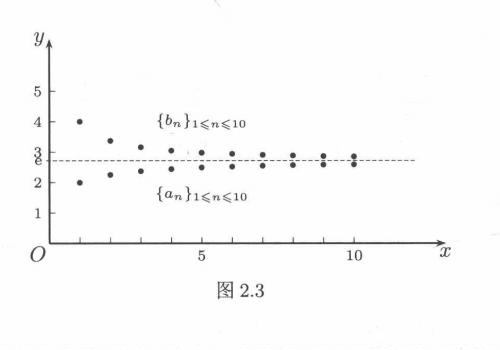
\includegraphics[width=.56\linewidth]{figures/upper/ch02/fig-2-3.png}
\end{center}

\begin{xremark}
同时考虑两个数列的方法有一个优点，即可以得到后面的不等式 (2.16)。若只要证 $\{a_n\}$ 有上界，则有很多其他方法。例如，下面的构思见 [41]：由于
\[
  \left(1+\frac1n\right)^n\cdot\frac12\cdot\frac12
  <\left[\frac{n\left(1+\frac1n\right)+2\cdot\frac12}{n+2}\right]^{n+2}=1,
\]
可知 $\{a_n\}$ 以 4 为上界。（用此法还可证明 $\{a_n\}$ 以 $\{b_n\}$ 的每一项为上界，其中即有 $b_1=4$。）
\end{xremark}

\textbf{证 2}\quad 将数列的通项 $a_n$ 用二项式展开，得到
\begin{align*}
  a_n
  &=1+\sum_{k=1}^n\binom nk\frac1{n^k}\\
  &=1+1+\frac1{2!}\left(1-\frac1n\right)
    +\frac1{3!}\left(1-\frac1n\right)\left(1-\frac2n\right)+\cdots\\
  &\quad+\frac1{n!}\left(1-\frac1n\right)\left(1-\frac2n\right)\cdots\left(1-\frac{n-1}{n}\right).
\end{align*}
比较 $a_n$ 和 $a_{n+1}$ 的类似展开式，可以看出前两项相同，而从第三项起，$a_{n+1}$ 的展开式中的每一项都比 $a_n$ 的展开式中的相应项来得大，而且最后还要多出一个正项，因此 $\{a_n\}$ 是严格单调增加数列。又可以用上述展开式作如下估计：
\[
  a_n<1+\frac1{1!}+\frac1{2!}+\frac1{3!}+\cdots+\frac1{n!}
  <1+1+\frac12+\frac1{2^2}+\cdots+\frac1{2^{n-1}}<3,
\]
因此 $\{a_n\}$ 有上界，从而收敛。
\end{xproof}

将上一命题中确定的极限记为 $\ee$，它的近似值是 $2.718\,281\,828\cdots$。在 1728 年大数学家 Euler 引入 $\ee$ 作为自然对数的底（见 [29]）。在本书中将自然对数 $\log_{\ee}x$ 记为 $\ln x$，在其他文献中也有记为 $\log x$ 的。从以后的学习中可以看到，虽然在日常计算中一般用常用对数，但在数学中用自然对数更为“自然”和方便得多。

下一命题表明数 $\ee$ 又是另一个数列的极限，它也称为 $\ee$ 的无穷级数展开式。

\begin{xproposition}[2.5.2]
证明数
\[
  \ee=\sum_{n=0}^{\infty}\frac1{n!}
  =1+1+\frac1{2!}+\frac1{3!}+\cdots+\frac1{n!}+\cdots.
\]
（记号 $\displaystyle\sum_{n=0}^{\infty}\frac1{n!}$ 是以 $\dfrac1{n!}$ 为通项的无穷级数，其中 $0!=1$。级数的和定义为部分和数列 $\{s_n\}$ 的极限，其中 $s_n=1+\dfrac1{1!}+\dfrac1{2!}+\cdots+\dfrac1{n!}$。参见例题 2.2.9 的注。）
\end{xproposition}
\begin{xproof}
从上一命题中已知 $\{s_n\}$ 以 $3$ 为上界，又因 $\{s_n\}$ 严格单调增加，因此收敛。记其极限为 $s$，则从 $a_n<s_n$ 得到 $\ee\le s$。固定正整数 $m$，并令 $n>m$，就有
\begin{align*}
  a_n
  &=1+1+\frac1{2!}\left(1-\frac1n\right)+\cdots
  +\frac1{n!}\left(1-\frac1n\right)\left(1-\frac2n\right)\cdots\left(1-\frac{n-1}{n}\right)\\
  &>1+1+\frac1{2!}\left(1-\frac1n\right)+\cdots
  +\frac1{m!}\left(1-\frac1n\right)\left(1-\frac2n\right)\cdots\left(1-\frac{m-1}{n}\right).
\end{align*}
其中不等号右边的和式是从 $a_n$ 的表达式中去掉后 $n-m$ 个正项得到的。令 $n\to\infty$，就有
\[
  \ee\ge1+1+\frac1{2!}+\frac1{3!}+\cdots+\frac1{m!}=s_m.
\]
再令 $m\to\infty$，得到 $\ee\ge s$。因此有 $s=\ee$。
\end{xproof}

\begin{xproposition}[2.5.3]
记
\[
  \varepsilon_n=\ee-\left(1+1+\frac1{2!}+\cdots+\frac1{n!}\right),
\]
则有 $\displaystyle\lim_{n\to\infty}\varepsilon_n(n+1)!=1$。
\end{xproposition}
\begin{xproof}
写出
\[
  \lim_{n\to\infty}\varepsilon_n(n+1)!
  =\lim_{n\to\infty}\frac{\varepsilon_n}{1/(n+1)!},
\]
然后用 $\dfrac00$ 型的 Stolz 定理（即命题 2.4.2）。这时
\[
  \varepsilon_{n+1}-\varepsilon_n=-\frac1{(n+1)!},
  \qquad
  \frac1{(n+2)!}-\frac1{(n+1)!}=-\frac1{n!(n+2)},
\]
可见所求的极限为 1。
\end{xproof}

这个结果也可以从下面更为精细的估计得出。

\begin{xproposition}[2.5.4]
对于上述 $\varepsilon_n$ 成立不等式
\[
  \frac1{(n+1)!}<\varepsilon_n<\frac1{n!\,n}.
\]
\end{xproposition}
\begin{xproof}
从
\[
  \varepsilon_n=\sum_{k=n+1}^{\infty}\frac1{k!}
\]
可见 $\varepsilon_n>\dfrac1{(n+1)!}$ 成立。对任意的 $m>n$，估计
\begin{align*}
  \frac1{(n+1)!}+\frac1{(n+2)!}+\cdots+\frac1{m!}
  &<\frac1{(n+1)!}\left(1+\frac1{n+2}+\cdots+\frac1{(n+2)^k}+\cdots\right)\\
  &=\frac1{(n+1)!}\left(\frac1{1-1/(n+2)}\right)\\
  &=\frac{n+2}{(n+1)!(n+1)}<\frac1{n!\,n}.
\end{align*}
再令 $m\to\infty$，就得到所求的第二个不等式。
\end{xproof}

现在证明关于数 $\ee$ 的一个基本结果，它也是 Euler 首先得到的。

\begin{xproposition}[2.5.5]
自然对数的底 $\ee$ 是无理数。
\end{xproposition}
\begin{xproof}
用反证法。如果 $\ee$ 是有理数，则可写为 $\ee=p/q$，这里 $p$ 和 $q$ 是正整数。从上两个命题知道，对于正整数 $q$，可以将 $\ee$ 的无穷级数展开式写成为两项之和，即从级数的第一项到 $1/q!$ 为第一部分，余下的 $\varepsilon_q$ 为第二部分：
\begin{equation}
  \ee=\frac pq
  =\left(1+\frac1{1!}+\frac1{2!}+\frac1{3!}+\cdots+\frac1{q!}\right)+\varepsilon_q.
  \tag{2.14}
  \label{eq:2.14}
\end{equation}
由此可见，$\varepsilon_q$ 一定是 $1/q!$ 的整数倍。但从上一个命题对 $\varepsilon_q$ 的估计知道，有
\[
  0<\varepsilon_q<\frac1{q!\,q},
\]
因此这是不可能的。
\end{xproof}

\begin{xremark}
\textbf{注 1}\quad 换一个写法，对不等式
\[
  0<\frac pq-\left(1+\frac1{1!}+\frac1{2!}+\cdots+\frac1{q!}\right)<\frac1{q!q}
\]
的两边同乘 $q!q$，则可见在中间的一个整数的值介于 0 和 1 之间，引出矛盾。

\textbf{注 2}\quad 在 1873 年数学家 Hermite（埃尔米特）进一步证明 $\ee$ 是超越数，也就是说 $\ee$ 不是任何一个整系数代数方程的根。这个证明可以在 [53, 55] 中找到。
\end{xremark}

本小节的前两个命题给出了以 $\ee$ 为极限的两个数列。在计算 $\ee$ 的近似值时用它的无穷级数展开式的前有限项之和有很多优点：计算方便，收敛快，又有很好的误差估计。如果用 $a_n=\left(1+\dfrac1n\right)^n$ 来计算 $\ee$，情况很不一样。若令
\[
  \delta_n=\ee-\left(1+\frac1n\right)^n,
\]
那么从本小节的命题 2.5.1 的证 1 可知
\[
  \delta_n<\left(1+\frac1n\right)^{n+1}-\left(1+\frac1n\right)^n
  =\left(1+\frac1n\right)^n\cdot\frac1n<\frac\ee n<\frac3n.
\]
进一步还可以得到
\[
  \lim_{n\to\infty}\frac{2n\delta_n}{\ee}=1,
\]
也就是说有
\begin{equation}
  \delta_n\sim\frac\ee{2n},
  \tag{2.15}
  \label{eq:2.15}
\end{equation}
其证明见例题 8.1.4。

用 $\{a_n\}$ 计算 $\ee$ 的近似值的实际例子：在取 $n=100$ 时，$a_{100}=2.70\cdots$，只有两位数字是正确的。又取 $n=10^4$，则有 $a_{10^4}=2.718\,14\cdots$，也只有四位数字是正确的。这里的误差与公式 (2.15) 的估计是一致的。另一方面，若用
\[
  s_n=1+\frac1{1!}+\frac1{2!}+\frac1{3!}+\cdots+\frac1{n!}
\]
来求 $\ee$ 的近似值，则在取 $n=10$ 时就有 $s_{10}=2.718\,281\,8\cdots$，所写出的八位数字都是正确的。这与命题 2.5.4 给出的误差估计也是一致的。关于收敛的速度和计算效率的研究将在计算方法课程中学习。数学分析为此提供了基础。

\paragraph{小结}
数 $\ee$ 的引进和研究是一个重要范例。这表明通过极限理论可以发现新的数。应当指出，由于这些数是通过极限来定义的，对它们的研究就很不容易。在这方面还有许多我们所不了解的东西，有待今后的研究。例如，虽然已经证明了 $\ee$ 和 $\pi$ 都是无理数和超越数，但迄今为止还没有人能证明 $\ee+\pi$ 是无理数。

\subsection{\texorpdfstring{Euler 常数 $\gamma$}{Euler 常数 gamma}}

\begin{xproposition}[2.5.6]
数列 $\{c_n\}$ 收敛，其中
\[
  c_n=1+\frac12+\cdots+\frac1n-\ln n,\qquad n\in\NN_+.
\]
\end{xproposition}
\begin{xproof}
这里需要用不等式
\begin{equation}
  \frac1{n+1}<\ln\left(1+\frac1n\right)<\frac1n,
  \tag{2.16}
  \label{eq:2.16}
\end{equation}
这可从命题 2.5.1 中建立的
\[
  \left(1+\frac1n\right)^n<\ee<\left(1+\frac1n\right)^{n+1}
\]
取自然对数得到。

现在研究数列 $\{c_n\}$ 的前后两项之差。由 (2.16) 的第一个不等式可见
\[
  c_{n+1}-c_n=\frac1{n+1}-\ln(n+1)+\ln n
  =\frac1{n+1}-\ln\left(1+\frac1n\right)<0,
\]
因此 $\{c_n\}$ 是严格单调减少数列。以下只要证明这个数列有下界即可。

在 (2.16) 的右边的不等式中将 $n$ 用 $1,2,\cdots,n$ 代入，然后将这些不等式相加，就得到
\[
  1+\frac12+\cdots+\frac1n>\ln(n+1)
  =\ln n+\ln\left(1+\frac1n\right)>\ln n+\frac1{n+1}.
\]
因此有
\[
  c_n=1+\frac12+\cdots+\frac1n-\ln n>\frac1{n+1}>0,
\]
可见数列 $\{c_n\}$ 为正数列，因此收敛。
\end{xproof}

\begin{xremark}
在确立了数列 $\{c_n\}$ 单调减少之后，也可以如同命题 2.5.1 的证 1 那样，引入第二个数列 $\{d_n\}$，其中
\[
  d_n=1+\frac12+\cdots+\frac1n-\ln(n+1),\qquad n\in\NN_+.
\]
这时有 $d_n<c_n,\ \forall n\in\NN_+$，且由 (2.16) 知 $c_n-d_n\to0$。同样可由 (2.16) 得到
\[
  d_{n+1}-d_n=\frac1{n+1}-\ln(n+2)+\ln(n+1)
  =\frac1{n+1}-\ln\left(1+\frac1{n+1}\right)>0.
\]
因此 $\{d_n\}$ 是严格单调增加数列，且有 $d_1<\cdots<d_n<c_n<\cdots<c_1$，$\forall n\in\NN_+$。因此数列 $\{c_n\}$ 以每个 $d_n$ 为下界，且和 $\{d_n\}$ 收敛于同一极限。
\end{xremark}

称以上数列 $\{c_n\}$ 的极限为 Euler 常数（或 Euler--Mascheroni（马斯凯罗尼）常数），记为
\[
  \gamma=\lim_{n\to\infty}\left(1+\frac12+\cdots+\frac1n-\ln n\right)
  \approx0.577\,215\,664.
\]
由上述命题，我们得到
\[
  1+\frac12+\cdots+\frac1n=\ln n+\gamma+\littleo(1).
\]

用这个公式和 Euler 常数的近似值就可以近似估计例题 2.2.6 中的发散数列 $\{S_n\}$ 当 $n$ 很大时的值。例如，在 $n=10^6$ 时，从
\[
  S_{10^6}=\sum_{k=1}^{10^6}\frac1k\approx6\ln10+\gamma,
\]
就得到 $S_{10^6}\approx14.392\,726$。用 Mathematica 软件验算，知道这 8 位数字都是准确的。实际上如用近似公式
\[
  1+\frac12+\cdots+\frac1n\approx\ln n+\gamma+\frac1{2n},
\]
则效果还要好得多。关于这方面的材料可以参考 [66]。

一个尚未解决的问题是：Euler 常数 $\gamma$ 是不是无理数？类似的问题在数学中还有很多。有人称 Euler 常数是其中“最大的谜”（见 [9] 中的 260 和 262 页）。

\subsection{例题}

\begin{xexample}[2.5.3]
证明 $\displaystyle\lim_{n\to\infty}\frac n{\sqrt[n]{n!}}=\ee$。
\end{xexample}
\begin{xproof}
\textbf{证 1}\quad 将 $\dfrac n{\sqrt[n]{n!}}$ 取对数，则只需证明其极限等于 1。经整理后得到
\[
  \ln\frac n{\sqrt[n]{n!}}
  =\frac{n\ln n-(\ln2+\ln3+\cdots+\ln n)}n
  =\frac{b_n}{n}.
\]
用 Cauchy 命题即知（也就是 2.4.3 小节的题 4）：
\[
  \lim_{n\to\infty}(b_{n+1}-b_n)=l
  \Longrightarrow
  \lim_{n\to\infty}\frac{b_n}{n}=l,
\]
计算得到
\[
  b_{n+1}-b_n=n\ln\left(1+\frac1n\right)
  =\ln\left(1+\frac1n\right)^n,
\]
可见极限为 1。

\textbf{证 2}\quad 将 $\dfrac n{\sqrt[n]{n!}}$ 改写为 $\sqrt[n]{\dfrac{n^n}{n!}}$，就可以用 2.4.3 小节题 6 中的方法来做。这时记 $a_n=\dfrac{n^n}{n!}$，因此只需计算后项与前项之比的极限：
\[
  \lim_{n\to\infty}\frac{a_{n+1}}{a_n}
  =\lim_{n\to\infty}\frac{(n+1)^{n+1}}{(n+1)!}\cdot\frac{n!}{n^n}
  =\lim_{n\to\infty}\left(1+\frac1n\right)^n=\ee.
\]
\end{xproof}

\begin{xremark}
利用下一小节题 7 中的不等式可以得到本题的又一个解法。此外，本题还有积分学解法（例题 11.4.2）。
\end{xremark}

\begin{xexample}[2.5.4]
计算极限
\[
  \lim_{n\to\infty}\left(\frac1{n+1}+\frac1{n+2}+\cdots+\frac1{2n}\right).
\]
\end{xexample}
\begin{xsolution}
从 Euler 常数的讨论知道，以
\[
  c_n=1+\frac12+\cdots+\frac1n-\ln n
\]
为通项的数列收敛。因此就知道 $\displaystyle\lim_{n\to\infty}(c_{2n}-c_n)=0$，又有
\[
  c_{2n}-c_n=\frac1{n+1}+\frac1{n+2}+\cdots+\frac1{2n}-\ln2,
\]
因此就求出
\[
  \lim_{n\to\infty}\left(\frac1{n+1}+\frac1{n+2}+\cdots+\frac1{2n}\right)
  =\lim_{n\to\infty}(c_{2n}-c_n)+\ln2=\ln2.
\]
\end{xsolution}

\begin{xremark}
此题的另一巧妙解法见 2.8.3 小节中的例题 4。此外本题在学了积分学后就只是一个常规练习题（参见例题 11.4.1）。
\end{xremark}

\subsection{练习题}

\begin{xexercise}[1]
计算下列极限：
  \begin{enumerate}[label=(\arabic*)]
    \item $\displaystyle\lim_{n\to\infty}\left(1-\frac1n\right)^n$；
    \item $\displaystyle\lim_{n\to\infty}\left(1+\frac1{2n}\right)^n$；
    \item $\displaystyle\lim_{n\to\infty}\left(1+\frac2n\right)^n$；
    \item $\displaystyle\lim_{n\to\infty}\left(1+\frac1n\right)^{n^2}$；
    \item $\displaystyle\lim_{n\to\infty}\left(1+\frac1{n^2}\right)^n$；
    \item $\displaystyle\lim_{n\to\infty}\left(1+\frac1n+\frac1{n^2}\right)^n$。
  \end{enumerate}

  \begin{xremark}
  在计算中可以应用 2.1.5 小节题 4 中有关连续性的结果。但是要请读者注意，在现阶段如下的做法是缺乏根据的（以题 (3) 为例）：
  \[
    \lim_{n\to\infty}\left(1+\frac2n\right)^n
    =\lim_{n\to\infty}\left[\left(1+\frac2n\right)^{n/2}\right]^2
    =\ee^2.
  \]
  \end{xremark}
\end{xexercise}
\begin{xsolution}
利用
\[
  \frac{x}{1+x}<\ln(1+x)<x\qquad(x>0)
\]
及本章已经建立的 $\left(1+1/n\right)^n\to\ee$，可得到：
\begin{enumerate}[label=(\arabic*)]
  \item 令 $m=n-1$，
  \[
    \left(1-\frac1n\right)^n
    =\left(1+\frac1m\right)^{-(m+1)}\to\ee^{-1}.
  \]
  \item
  \[
    \left(1+\frac1{2n}\right)^n
    =\left[\left(1+\frac1{2n}\right)^{2n}\right]^{1/2}\to\ee^{1/2}.
  \]
  \item 由上述对数不等式，
  \[
    \frac{2n}{n+2}
    <n\ln\left(1+\frac2n\right)<2.
  \]
  两端都趋于 $2$，故
  \[
    n\ln\left(1+\frac2n\right)\to2,
  \]
  从而
  \[
    \left(1+\frac2n\right)^n\to\ee^2.
  \]
  \item
  \[
    \left(1+\frac1n\right)^{n^2}
    =\left[\left(1+\frac1n\right)^n\right]^n\to+\infty,
  \]
  因为括号内最终大于某个常数 $q>1$。
  \item 取对数，有
  \[
    0<n\ln\left(1+\frac1{n^2}\right)<\frac1n\to0,
  \]
  故极限为 $1$。
  \item 取对数并令 $u_n=1/n+1/n^2$，则
  \[
    \frac{nu_n}{1+u_n}<n\ln(1+u_n)<nu_n.
  \]
  两端均趋于 $1$，故对数趋于 $1$，原极限为 $\ee$。
\end{enumerate}
\end{xsolution}


\begin{xexercise}[2]
设 $k\in\NN_+$，证明：$\displaystyle\frac{k}{n+k}<\ln\left(1+\frac kn\right)<\frac kn$。
\end{xexercise}
\begin{xsolution}
把不等式 (2.16)
\[
  \frac1{j+1}<\ln\left(1+\frac1j\right)<\frac1j
\]
中的 $j$ 依次取 $n,n+1,\ldots,n+k-1$ 并相加，得到
\[
  \sum_{j=n}^{n+k-1}\frac1{j+1}
  <\ln\left(1+\frac kn\right)
  <\sum_{j=n}^{n+k-1}\frac1j.
\]
左边每项都不小于 $1/(n+k)$，右边每项都不大于 $1/n$，故
\[
  \boxed{\frac{k}{n+k}<\ln\left(1+\frac kn\right)<\frac kn}.
\]
\end{xsolution}


\begin{xexercise}[3]
求 $\displaystyle\lim_{n\to\infty}\left(1+\frac1{n^2}\right)\left(1+\frac2{n^2}\right)\cdots\left(1+\frac n{n^2}\right)$。
\end{xexercise}
\begin{xsolution}
记
\[
  P_n=\prod_{k=1}^n\left(1+\frac{k}{n^2}\right).
\]
取对数并用 $x/(1+x)<\ln(1+x)<x$：
\[
  \sum_{k=1}^n\frac{k/n^2}{1+k/n^2}
  <\ln P_n
  <\sum_{k=1}^n\frac{k}{n^2}.
\]
右端趋于 $1/2$。左右两端之差不超过
\[
  \sum_{k=1}^n\left(\frac{k}{n^2}\right)^2
  =\frac1{n^4}\sum_{k=1}^n k^2\to0.
\]
因此 $\ln P_n\to1/2$，从而
\[
  \boxed{P_n\to\sqrt\ee}.
\]
\end{xsolution}


\begin{xexercise}[4]
设 $\{p_n\}$ 是正数列，且 $p_n\to+\infty$，计算 $\displaystyle\lim_{n\to\infty}\left(1+\frac1{p_n}\right)^{p_n}$。
\end{xexercise}
\begin{xsolution}
令
\[
  y_n=\left(1+\frac1{p_n}\right)^{p_n}.
\]
由于 $p_n\to+\infty$，
\[
  \frac{p_n}{p_n+1}
  <p_n\ln\left(1+\frac1{p_n}\right)<1.
\]
两端趋于 $1$，故 $\ln y_n\to1$，于是
\[
  \boxed{y_n\to\ee}.
\]
\end{xsolution}


\begin{xexercise}[5]
求 $\displaystyle\lim_{n\to\infty}\frac{n!\,2^n}{n^n}$。
\end{xexercise}
\begin{xsolution}
令
\[
  u_n=\frac{n!\,2^n}{n^n}>0.
\]
由本章例题 2.5.3，
\[
  \sqrt[n]{u_n}=2\frac{\sqrt[n]{n!}}n\to\frac2\ee<1.
\]
取 $q$ 满足 $2/\ee<q<1$，则充分大的 $n$ 有 $\sqrt[n]{u_n}<q$，从而 $0<u_n<q^n\to0$。故极限为 $0$。
\end{xsolution}


\begin{xexercise}[6]
求极限 $\displaystyle\lim_{n\to\infty}\frac{\ln n}{1+\frac12+\cdots+\frac1n}$。
\end{xexercise}
\begin{xsolution}
由 Euler 常数的定义，
\[
  H_n=1+\frac12+\cdots+\frac1n
  =\ln n+\gamma+\littleo(1).
\]
故
\[
  \frac{\ln n}{H_n}
  =\frac1{1+(\gamma+\littleo(1))/\ln n}\to1.
\]
\end{xsolution}


\begin{xexercise}[7]
证明：
  \[
    \left(\frac{n+1}{\ee}\right)^n<n!<\ee\left(\frac{n+1}{\ee}\right)^{n+1}.
  \]
  （由此又可得到 $\displaystyle\lim_{n\to\infty}\frac n{\sqrt[n]{n!}}=\ee$。）
\end{xexercise}
\begin{xsolution}
由 (2.16)，对 $k=1,\ldots,n$ 有
\[
  \frac{k}{k+1}<k\ln\left(1+\frac1k\right)<1.
\]
相加得
\[
  n+1-H_{n+1}
  <\sum_{k=1}^n k\ln\left(1+\frac1k\right)<n.
\]
而
\[
  \sum_{k=1}^n k\ln\left(1+\frac1k\right)
  =n\ln(n+1)-\ln n!.
\]
上界立即给出
\[
  \ln n!>n\ln(n+1)-n,
\]
即
\[
  \left(\frac{n+1}{\ee}\right)^n<n!.
\]

另一方面，由 $H_{n+1}<1+\ln(n+1)$，上面的下界给出
\[
  n\ln(n+1)-\ln n!>n-\ln(n+1).
\]
整理为
\[
  \ln n!<(n+1)\ln(n+1)-n,
\]
即
\[
  n!<\ee\left(\frac{n+1}{\ee}\right)^{n+1}.
\]
\end{xsolution}


\begin{xexercise}[8]
设 $S_n=1+2^2+3^3+\cdots+n^n$，$n\in\NN_+$。证明：对 $n\ge2$，成立不等式
  \[
    n^n\left[1+\frac1{4(n-1)}\right]\le S_n
    <n^n\left[1+\frac2{\ee(n-1)}\right].
  \]
\end{xexercise}
\begin{xsolution}
记 $S_n=\sum_{k=1}^n k^k$。显然
\[
  S_n\ge n^n+(n-1)^{n-1}.
\]
由
\[
  \left(1+\frac1{n-1}\right)^{n-1}<\ee
\]
得
\[
  (n-1)^{n-1}>\frac{n^{n-1}}\ee.
\]
对 $n\ge4$，$1/\ee\ge n/[4(n-1)]$，故
\[
  (n-1)^{n-1}\ge\frac{n^n}{4(n-1)}.
\]
$n=2,3$ 可直接检查，所以
\[
  S_n\ge n^n\left(1+\frac1{4(n-1)}\right).
\]

再看上界。对 $2\le k\le n$，
\[
  \frac{(k-1)^{k-1}}{k^k}<\frac1k\le\frac12.
\]
因此
\[
  1^1+2^2+\cdots+(n-1)^{n-1}<2(n-1)^{n-1}.
\]
又由
\[
  \ee<\left(1+\frac1{n-1}\right)^n
\]
可得
\[
  (n-1)^{n-1}<\frac{n^n}{\ee(n-1)}.
\]
于是
\[
  S_n<n^n\left(1+\frac2{\ee(n-1)}\right).
\]
两边不等式均得证。
\end{xsolution}


\begin{xexercise}[9]
设有 $a_1=1$，$a_n=n(a_{n-1}+1)$，$n=2,3,\cdots$，又设
  \[
    x_n=\prod_{k=1}^n\left(1+\frac1{a_k}\right),\qquad n\in\NN_+,
  \]
  求数列 $\{x_n\}$ 的极限。
\end{xexercise}
\begin{xsolution}
令
\[
  b_n=\frac{a_n}{n!}.
\]
由 $a_n=n(a_{n-1}+1)$，
\[
  b_n=b_{n-1}+\frac1{(n-1)!},
\]
且 $b_1=1$，故
\[
  b_n=\sum_{j=0}^{n-1}\frac1{j!}.
\]
另一方面，
\[
  1+\frac1{a_k}
  =\frac{a_k+1}{a_k}
  =\frac{a_{k+1}}{(k+1)a_k}.
\]
所以乘积望远镜相消：
\[
  x_n=\prod_{k=1}^n\left(1+\frac1{a_k}\right)
  =\frac{a_{n+1}}{(n+1)!}=b_{n+1}.
\]
于是
\[
  \boxed{x_n\to\ee}.
\]
\end{xsolution}


\section{由迭代生成的数列}

这里所说的“由迭代生成的数列”是指在给出数列的第一项 $a_1$ 后，用递推公式
\[
  a_{n+1}=f(a_n)\quad(n\in\NN_+)
\]
通过迭代生成的数列。这里只讨论函数 $f$ 与 $n$ 无关的情况。这样的数列在数学和其他领域中经常出现，有很强的理论和实用价值。例如，大量的近似计算方法都是用迭代方式来实现的（一个具体例子就是本书 §8.7 的方程求根算法）。同时这类数列有很强的共同规律，又与 20 世纪 60、70 年代中期发展起来的混沌研究直接有关。本节将对此作一个基本介绍，重点是几何方法。

在下一章学了 Cauchy 收敛准则后，将进一步介绍处理迭代生成数列的另一种方法——压缩映射原理，并且用这个原理对下一小节中的两个例题给出新的解法。此外，在那里还会看到，上、下极限也是处理迭代生成数列的有用工具。

\subsection{例题}

\begin{xexample}[2.6.1]
设 $a_1=\sqrt2$，$a_{n+1}=\sqrt{2+a_n}$，$n\in\NN_+$。讨论数列 $\{a_n\}$ 的敛散性，若收敛则求出其极限。

（本题的另一种形式是求极限 $\displaystyle\lim_{n\to\infty}\sqrt{2+\sqrt{2+\cdots+\sqrt2}}$，其中根号共 $n$ 重；这时的第一步就是将数列写成递推形式。）
\end{xexample}
\begin{xsolution}
可以归纳地证明这个数列是严格单调增加的，并且以 2 为上界。实际上，从递推公式和初始值为正就可推知数列的每一项为正。从
\[
  a_1=\sqrt2<\sqrt{2+\sqrt2}=a_2,
\]
以及
\[
  a_{n-1}<a_n\Longrightarrow
  a_n=\sqrt{2+a_{n-1}}<\sqrt{2+a_n}=a_{n+1},
\]
可见数列是单调增加的。又从 $a_1<2$ 和
\[
  a_n<2\Longrightarrow a_{n+1}=\sqrt{2+a_n}<\sqrt{2+2}=2,
\]
可见数列以 2 为上界。因此它是收敛数列。记极限是 $a$。在递推公式 $a_{n+1}=\sqrt{2+a_n}$ 的两边令 $n\to\infty$，就得到关于 $a$ 的方程
\[
  a=\sqrt{2+a}.
\]
因 $a>0$，该方程只有一个正解 $a=2$，这就是所要求的极限。
\end{xsolution}

\begin{xremark}
这里介绍证明 $\{a_n\}$ 有上界的另一个方法。它在处理 $a_n$ 中出现 $n$ 重根式的类似问题时可能有用。利用
\[
  \sqrt{2+\sqrt2}<\sqrt{2+2}=2,
\]
就可以在 $a_n$ 的表达式 $\sqrt{2+\sqrt{2+\cdots+\sqrt2}}$ 中从最里面开始，从内到外将根号逐个脱去，得到 $a_n<2$。
\end{xremark}

\paragraph{问题}
在上述简单例题中是否包含了迭代生成数列所共有的某些普遍规律？例如，这样的数列是否都是单调的？上界 2 与答案相同是否偶然？求极限的方法是否都是如此？总而言之，迭代生成数列的收敛与求其极限是否有普遍适用的方法？在下一小节我们将要回答这些问题。在此之前，再看一个例题。它说明迭代生成的数列不一定是单调的。但这里仍然有规律。

\begin{xexample}[2.6.2]
数列 $\{b_n\}$ 由 $b_1=1$ 和 $b_{n+1}=1+\dfrac1{b_n}$（$n\in\NN_+$）生成。讨论 $\{b_n\}$ 的敛散性，若收敛则求出其极限。
\end{xexample}
\begin{xsolution}
先假定数列 $\{b_n\}$ 收敛，记极限为 $b$。从迭代所用的递推公式中令 $n\to\infty$，就得到 $b^2-b-1=0$。它有两个根：$(1\pm\sqrt5)/2$。由于容易归纳地看出所有的 $b_n>0$，因此如果存在极限，则只能是 $b=(1+\sqrt5)/2\approx1.618$。

考虑数列 $\{b_n\}$ 中的项 $b_n$ 和 $b_{n+2}$ 的关系。可以从递推公式导出 $b_{n+2}=2-1/(b_n+1)$。由于上面求出的 $b$ 也满足等式 $b=2-1/(b+1)$，就有
\begin{equation}
  b_{n+2}-b=\frac{b_n-b}{(b_n+1)(b+1)}.
  \tag{2.17}
  \label{eq:2.17}
\end{equation}
可见，$b_n-b$ 和 $b_{n+2}-b$ 总是同号的。利用 $b$ 的近似值 1.618 和 $b_1=1,b_2=2$，就知道对每个 $k$ 均成立 $b_{2k-1}<b<b_{2k}$。直接研究差值
\[
  b_{n+2}-b_n=\frac{b_n-b_{n-2}}{(b_n+1)(b_{n-2}+1)},
\]
并计算出数列的前几项 $b_1=1,b_2=2,b_3=1.5,b_4=1.666\cdots$，可见 $\{b_{2k-1}\}$ 严格单调增加，$\{b_{2k}\}$ 严格单调减少，而且有
\[
  b_1<b_3<\cdots<b<\cdots<b_4<b_2,
\]
因此它们都是收敛数列。在它们共同的递推公式 $b_{n+2}=2-\dfrac1{b_n+1}$ 中令 $n\to\infty$，可见它们的极限都是 $b$。因此数列 $\{b_n\}$ 收敛于 $b$。
\end{xsolution}

\begin{xremark}
顺便指出本题与 Fibonacci（斐波那契）数列有关。所谓 Fibonacci 数列，即是由
\[
  F_1=1,\quad F_2=1,\quad F_{n+2}=F_{n+1}+F_n,\qquad n\in\NN_+,
\]
确定的数列 $\{F_n\}$。它的前 12 项是 $1,1,2,3,5,8,13,21,34,55,89,144$。如果要求其中相继两项的增长率的极限，即 $\displaystyle\lim_{n\to\infty}(F_{n+1}/F_n)$，则从
\[
  \frac{F_{n+1}}{F_n}=\frac{F_n+F_{n-1}}{F_n}
  =1+\frac1{F_n/F_{n-1}}
\]
可见，这个极限就是上一个例题中求出的答案：$\dfrac{\sqrt5+1}{2}\approx1.618$。
\end{xremark}

很自然会产生这样的问题：例题 2.6.2 的解法是怎样想出来的？为什么会去研究 $b_{n+2}$ 和 $b_n$ 的关系？

实际上与很多其他例题一样，写在书本上的解答与实际的思维过程可能完全不同。对本题的一般思维过程是先计算数列 $\{b_n\}$ 的前几项，发现它们有（例如）以下的大小关系：
\[
  b_1<b_3<b_5<\cdots<b_6<b_4<b_2,
\]
然后（可能会提出）猜测：$\{b_{2k-1}\}$ 可能单调增加，$\{b_{2k}\}$ 可能单调减少。又假定数列收敛，求出 $b$，由此想到去研究 $b_{n+2}-b$ 和 $b_{n+2}-b_n$。注意，这里由几个特例作出猜测的方法是在科学研究中（不仅仅在数学中）普遍采用的归纳法。但这不是数学归纳法。数学归纳法是用来证明与正整数有关的命题 $P(n)$ 成立的严格的数学方法，也称为完全归纳法。一旦证明成功，命题就成立了。但上面所说的归纳法并非如此，它更接近于科学研究中的一般思维方法。从几个特例总结出来的命题可能对，也可能错，因此有时也称为不完全归纳法。在这一点上说，它似乎不如数学归纳法。但实际上数学归纳法只是证明命题的一种严格的数学方法，至于这个命题从何处得来，（在证明成功之前）命题成立的可能性如何，数学归纳法对此是无能为力的。从不完全归纳法提出的猜测也被称为似然猜想，在 Pólya 的 [46] 中有系统的论述。该书和 [45, 47] 一起，是有关数学思维和数学教育方面的名著。在这方面还可以参考 [49]。

实际上，上面两个例题中的确包含了许多迭代生成数列的共同规律，如果掌握了这些规律，就有可能更有效地处理同样类型的问题。

\subsection{单调性与几何方法}

关于迭代生成数列的第一个规律可概括在下列命题中。

\begin{xproposition}[2.6.1（第一律）]
设数列 $\{x_n\}$ 满足递推公式 $x_{n+1}=f(x_n)$，$n\in\NN_+$。若有 $\displaystyle\lim_{n\to\infty}x_n=\xi$，同时又成立
\begin{equation}
  \lim_{n\to\infty}f(x_n)=f(\xi),
  \tag{2.18}
  \label{eq:2.18}
\end{equation}
则极限 $\xi$ 一定是方程 $f(x)=x$ 的根（这时称 $\xi$ 为函数 $f$ 的不动点）。
\end{xproposition}

\begin{xremark}
这个命题的证明是简单的，只不过是在递推公式 $x_{n+1}=f(x_n)$ 的两边令 $n\to\infty$ 而已。这在上面两个例题中都已这样做过。命题中的条件 (2.18) 在今后学了函数的连续性概念后可替换为 $f$ 在点 $\xi$ 处连续或在更大的范围上连续等条件。（从第五章连续函数中的 Heine（海涅）归结原理知道，函数 $f$ 在点 $a$ 处连续的充分必要条件就是对每个收敛于 $a$ 的数列 $\{a_n\}$，成立 $\displaystyle\lim_{n\to\infty}f(a_n)=f(a)$。）

这个命题的用处是明显的。它使我们在还不知道数列的收敛情况之前，就可以先去求解方程 $f(x)=x$。求出方程的根对判定原数列的收敛性往往会有帮助。例如，如果方程 $f(x)=x$ 在实数范围中无根，则无须再作任何研究就可以断定：这个迭代生成数列一定发散（见前面的例题 2.2.8）。又如在上面的例题 2.6.2 中，一开始就求出 $b$，到最后才证明它是极限。我们已经看到在该题的求解中 $b$ 所起的作用。
\end{xremark}

关于迭代生成数列的第二个规律是它的单调性。如果假定在递推公式中的函数 $f$ 为单调函数，则很容易证明只有两种可能情况：(1) 这个数列是单调的；(2) 这个数列的奇数项子列和偶数项子列分别是单调的，而且具有相反的单调性。事实上，在数学分析课程中见到的这类数列的绝大多数都合乎这个规律。这就是下一个命题。请注意其中既不要求数列收敛，也不要求它有界（区间 $I$ 可以无界）。

\begin{xproposition}[2.6.2（第二律）]
设 $\{x_n\}$ 满足关系 $x_{n+1}=f(x_n)$，$n\in\NN_+$，其中的函数 $f$ 在区间 $I$ 上单调，同时数列 $\{x_n\}$ 的每一项都在区间 $I$ 中，则只有两种可能：(1) 当 $f$ 单调增加时，$\{x_n\}$ 为单调数列；(2) 当 $f$ 单调减少时，$\{x_n\}$ 的两个子列 $\{x_{2k-1}\}$ 和 $\{x_{2k}\}$ 分别为单调数列，且具有相反的单调性。
\end{xproposition}
\begin{xproof}
分别讨论命题中的两种情况。

(1) 设 $f(x)$ 在区间 $I$ 上单调增加。根据条件，有 $x_n\in I$，$n\in\NN_+$。观察数列的前两项。如有 $x_1\le x_2=f(x_1)$，则就有 $x_2=f(x_1)\le f(x_2)=x_3$。用数学归纳法可知，数列 $\{x_n\}$ 单调增加。完全类似地可以证明，在 $x_1>x_2$ 时，数列 $\{x_n\}$ 单调减少。

(2) 设 $f(x)$ 在区间 $I$ 上单调减少。注意：复合函数 $f(f(x))$ 却是单调增加的。严格地说，只要 $a,b\in I$，$a<b$，而且 $f(a),f(b)\in I$，就成立 $f(f(a))\le f(f(b))$。

观察 $x_1$ 与 $x_3$。如果 $x_1=x_3$，则子列 $\{x_{2k-1}\}$ 为常值数列。如成立 $x_1<x_3$，从 $f$ 单调减少就有 $x_2\ge x_4$，然后推出 $x_3\le x_5$。以下的讨论已无困难。用数学归纳法即可证明这时子列 $\{x_{2k-1}\}$ 单调增加。由于函数 $f$ 单调减少，从 $x_{2k}=f(x_{2k-1})$，$k\in\NN_+$，可知子列 $\{x_{2k}\}$ 单调减少。对于 $x_1>x_3$ 的讨论完全类似，从略。
\end{xproof}

\begin{xremark}
从证明中不难看出，以上的单调性还具有一个特点。举例来说，在 (1) 中的 $\{x_n\}$ 为单调增加的情况，只有两种可能性：或者是从某项之后为常值数列，或者是严格单调增加数列。
\end{xremark}

现在问题已经很清楚，如果迭代生成数列 $\{x_n\}$ 在函数 $f$ 的单调区间内而且有界的话（区间 $I$ 可以无界），则在情况 (1) 时数列必收敛，而在情况 (2) 时数列可能收敛，也可能发散，但两个子列 $\{x_{2k-1}\}$ 和 $\{x_{2k}\}$ 则一定收敛。因此问题取决于这两个子列的极限是否相等。对于数列无界的情况可以作出类似的讨论。

对于具体问题来说，应用以上两个规律的最简便方法就是作图。首先在坐标平面上作出函数 $y=f(x)$ 的图像。在命题 2.6.1 中的不动点就是曲线 $y=f(x)$ 和直线 $y=x$ 的交点。对于很多简单函数，不难确定它的单调区间。为了知道迭代生成数列的具体情况，往往不需要作很多计算，而只要用我们在下面介绍的作图法即可。它有一个很形象化的名称——蛛网（cobweb）工作法。

\begin{center}
  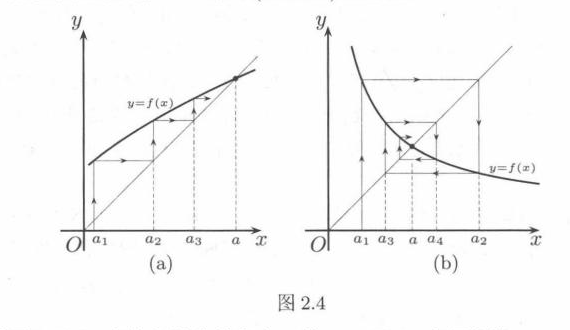
\includegraphics[width=.76\linewidth]{figures/upper/ch02/fig-2-4.png}
\end{center}

先看图 2.4(a)。在其中的曲线代表函数 $y=f(x)$。它同直线 $y=x$ 的交点的横坐标 $a$ 就是 $f$ 的不动点。从图中的 $x$ 轴上代表初始值 $a_1$ 的点出发作平行于 $y$ 轴的直线，它与曲线 $y=f(x)$ 的交点的纵坐标就是 $a_2=f(a_1)$。在这里的一个技巧是从上述交点作平行于 $x$ 轴的直线与直线 $y=x$ 相交，这个交点的横坐标当然也是 $a_2$。在图中从这个交点作一条虚线与纵轴平行，并将它与 $x$ 轴的交点标为 $a_2$。这就完成了蛛网工作法的第一步。

在图 2.4(a) 上将这个方法继续做几步，可以看出，所得的数列是单调增加的。这与命题 2.6.2 一致，它可能以 $a$ 为极限。当然要严格建立这些结论的话还要进行分析证明。但以上的几何观察在发现规律和提供思路上是很有用的。

将图 2.4(a) 中的想法严格化，就可以建立下面的命题。在这个命题中，对于 $f$ 在点 $a$ 的连续性条件，按照命题 2.6.1 的注解来理解。

\begin{xproposition}[2.6.3]
设 $a$ 是 $f(x)$ 的不动点，函数 $f$ 在 $a$ 处连续，在点 $a$ 的邻域 $(a-r,a+r)$ 上严格单调增加，并且在区间 $(a-r,a)$ 上有 $f(x)>x$，而在区间 $(a,a+r)$ 上有 $f(x)<x$，那么迭代生成数列只要第一项在 $(a-r,a+r)$ 内，且不等于 $a$，则以后就不会越出这个区间，而且是以 $a$ 为极限的严格单调数列。
\end{xproposition}
\begin{xproof}
从条件可知，$f$ 在点 $a$ 的两侧均有 $f(x)\ne x$，因此 $f$ 在区间 $(a-r,a+r)$ 内只可能有唯一的不动点 $a$。不妨设初始值 $a_1\in(a-r,a)$。从 $f$ 的严格单调性和 $a_1<a$ 得到 $a_2=f(a_1)<f(a)=a$。又因为在区间 $(a-r,a)$ 上满足条件 $f(x)>x$，就有 $a_2=f(a_1)>a_1$。合并起来就有 $a_1<a_2<a$。

用数学归纳法可以证明数列 $\{a_n\}$ 完全落在区间 $(a-r,a)$ 内，且严格单调增加。由于它以 $a$ 为上界，因此收敛。它的极限应当在区间 $[a_1,a]\subset(a-r,a]$ 内。由于在这里 $a$ 是唯一的不动点，因此极限就是 $a$。又类似地可以证明，在初始值 $a_1\in(a,a+r)$ 时，数列 $\{a_n\}$ 是以 $a$ 为极限的严格单调减少数列。
\end{xproof}

另一方面，如果将在区间 $(a-r,a)$ 上“$f(x)>x$”的条件改为“$f(x)<x$”，而保持其他条件不变，则当初始值 $a_1\in(a-r,a)$ 时，就有 $a_2=f(a_1)<a_1$。这样一来，在几次迭代之后就可能会越出 $(a-r,a)$，但在这之前是严格单调减少的。

另一方面，当函数 $f$ 在点 $a$ 附近为单调减少时，就可能出现第二种情况，它同样有明显的几何意义。这就是图 2.4(b) 中所表示的情况。这里数列 $\{a_n\}$ 的奇数项子列严格单调增加，而偶数项子列严格单调减少。当然为了迭代生成数列不越出 $f$ 的单调区间并收敛于不动点 $a$，这时对函数 $f$ 也需要加一定的条件才行（读者可自己写出具体的条件并加以分析论证）。

现在可以回答上一小节末提出的问题。我们解例题 2.6.2 的方法是先作一个类似于图 2.4(b) 那样的草图，其中的 $f(x)=1+\dfrac1x$，然后在图上使用蛛网工作法。这样就在写分析论证之前可以看出此题的迭代生成数列一定是第二律中的情况 (2)。剩下的就是通过细心的运算来写出证明而已。这个求解的书写恰如用数学归纳法一样，所要证明的结论是在证明之前用其他方法得到的。

以上所介绍的关于迭代生成数列的一些简单规律是许多科学家早就知道的，并在生态学等领域有实际应用。长期以来，没有人去考虑在这些规律性之外还会有什么值得研究。在 20 世纪 70 年代中期，开始有人对迭代生成数列进行大范围的研究，这是混沌科学开始发展的几个源头之一。在这里要指出，当函数 $y=f(x)$ 在定义域上并非单调时，在迭代过程中离开某个不动点的点完全可能再回到这个不动点附近，甚至直接落到这个或另一个不动点上，从而会出现极其复杂的行为。有兴趣的读者可以阅读生态学家 R. M. May（梅）的科普文章 [39]。该文强调了迭代生成数列在生物学、经济学和社会科学中的重要性，同时还呼吁将其中的最新发现放到初等数学的课程中去。此文在推动混沌学的发展上起过重要的作用。（参看本书的 §5.6。）

\subsection{练习题}

在以下各题中均可试用几何方法，或作出几何解释。

\begin{xexercise}[1]
\begin{enumerate}[label=(\arabic*)]
    \item 设 $a>0$，$x_1=\sqrt a$，$x_{n+1}=\sqrt{a+x_n}$，$n\in\NN_+$，求 $\displaystyle\lim_{n\to\infty}x_n$；
    \item 设 $a>0$，$x_1=\sqrt a$，$x_{n+1}=\sqrt{ax_n}$，$n\in\NN_+$，求 $\displaystyle\lim_{n\to\infty}x_n$。
  \end{enumerate}
  （这两题外形相似，都可用本节方法解决。但题 (2) 有更简单的直接解法。）
\end{xexercise}
\begin{xsolution}
(1) 令
\[
  L=\frac{1+\sqrt{1+4a}}2,
\]
则 $L>0$ 且 $L^2=L+a$。由于 $x_1=\sqrt a<L$，且函数 $f(x)=\sqrt{a+x}$ 单调增加；对 $0<x<L$，
\[
  x<f(x)<L.
\]
因此归纳可得 $0<x_1<x_2<\cdots<L$。数列单调有界，故收敛，极限只能是不动点 $L$。所以
\[
  \boxed{\lim x_n=\frac{1+\sqrt{1+4a}}2}.
\]

(2) 因所有项为正，令 $y_n=\ln x_n$。递推式变为
\[
  y_{n+1}=\frac{\ln a+y_n}{2},
  \qquad y_1=\frac12\ln a.
\]
直接解得
\[
  y_n=(1-2^{-n})\ln a\to\ln a.
\]
故
\[
  \boxed{x_n\to a}.
\]
\end{xsolution}


\begin{xexercise}[2]
设 $A>0$，$0<b_0<A^{-1}$，$b_{n+1}=b_n(2-Ab_n)$，$n\in\NN_+$。证明：$\displaystyle\lim_{n\to\infty}b_n=A^{-1}$。
\end{xexercise}
\begin{xsolution}
令
\[
  e_n=1-Ab_n.
\]
由 $0<b_0<A^{-1}$ 知 $0<e_0<1$。递推式给出
\[
  e_{n+1}=1-Ab_n(2-Ab_n)=(1-Ab_n)^2=e_n^2.
\]
因此
\[
  e_n=e_0^{2^n}\to0,
\]
从而
\[
  \boxed{b_n\to A^{-1}}.
\]
\end{xsolution}


\begin{xexercise}[3]
设参数 $b>4$，$x_1=\dfrac12$，$x_{n+1}=bx_n(1-x_n)$，$n\in\NN_+$。证明：$\{x_n\}$ 发散。
\end{xexercise}
\begin{xsolution}
因 $x_1=1/2$，有
\[
  x_2=\frac b4>1.
\]
于是
\[
  x_3=bx_2(1-x_2)<0.
\]
若 $x<0$，则
\[
  bx(1-x)<x,
\]
因为 $b(1-x)>b>4>1$，乘以负数 $x$ 后不等号反向。因此从 $x_3$ 起数列严格减少并保持负值。

若它有有限极限 $L$，连续性给出 $L=bL(1-L)$，即 $L=0$ 或 $L=1-1/b>0$，都与尾部严格为负且递减矛盾。因此数列无有限极限，实际上 $x_n\to-\infty$，故发散。
\end{xsolution}


\begin{xexercise}[4]
设 $x_1=b$，$x_{n+1}=\dfrac12(x_n^2+1)$。问：$b$ 取何值时数列 $\{x_n\}$ 收敛，并求其极限。
\end{xexercise}
\begin{xsolution}
有
\[
  x_{n+1}-x_n=\frac{(x_n-1)^2}{2}\ge0,
\]
所以数列总是单调不减。

若 $-1\le b\le1$，则 $x_2=(b^2+1)/2\in[1/2,1]$；以后若 $0\le x_n\le1$，就有 $x_n\le x_{n+1}\le1$。故数列收敛，其极限满足
\[
  L=\frac{L^2+1}{2},
\]
于是 $L=1$。

若 $\abs b>1$，则 $x_2>1$，以后严格增加。若有有限极限也只能为 $1$，但尾部始终大于 $1$ 且严格增加，不可能趋于 $1$，故发散于 $+\infty$。

因此
\[
  \boxed{\{x_n\}\text{ 收敛当且仅当 }-1\le b\le1,
  \quad\text{此时极限为 }1.}
\]
\end{xsolution}


\begin{xexercise}[5]
设 $x_0=a$，$x_n=1+bx_{n-1}$，$n\in\NN_+$。试求出使该数列收敛的 $a,b$ 的所有值。

  （本题为线性迭代，解法很多。）
\end{xexercise}
\begin{xsolution}
递推式为
\[
  x_n=1+bx_{n-1},\qquad x_0=a.
\]
若 $b\ne1$，其通项为
\[
  x_n=\frac1{1-b}+b^n\left(a-\frac1{1-b}\right).
\]
因此分类如下：
\begin{itemize}
  \item $\abs b<1$：任意 $a$ 均收敛，极限为 $1/(1-b)$；
  \item $b=-1$：只有 $a=1/2$ 时为常值数列并收敛；
  \item $\abs b>1$：只有 $a=1/(1-b)$ 时为常值数列并收敛；
  \item $b=1$：$x_n=a+n$，对任何 $a$ 都不收敛。
\end{itemize}
这就是全部可能情形。
\end{xsolution}


\begin{xexercise}[6]
（对于线性迭代的全面讨论）设给定初始值 $x_1$，然后用线性函数 $f(x)=ax+b$ 迭代生成数列 $\{x_n\}$，即 $x_{n+1}=ax_n+b$。试回答以下问题：
  \begin{enumerate}[label=(\arabic*)]
    \item 是否存在线性函数，使对于任何初始值 $x_1$，$\{x_n\}$ 总是收敛的？
    \item 是否存在线性函数，使对于任何初始值 $x_1$，$\{x_n\}$ 总是发散的？
    \item 是否存在线性函数，使对于不同的初始值 $x_1$，$\{x_n\}$ 收敛到不同极限？
    \item 是否存在线性函数，使对于某些初始值 $x_1$，$\{x_n\}$ 收敛，而对于其他初始值 $x_1$，$\{x_n\}$ 发散？
  \end{enumerate}
\end{xexercise}
\begin{xsolution}
线性迭代
\[
  x_{n+1}=ax_n+b
\]
在 $a\ne1$ 时满足
\[
  x_n=x_*+a^{n-1}(x_1-x_*),
  \qquad x_*=\frac b{1-a}.
\]
据此逐问回答：

(1) 存在。例如取 $\abs a<1$，则对任何 $x_1$ 都收敛于 $x_*$。

(2) 存在。例如取 $a=1,b=1$，则 $x_n=x_1+n-1\to+\infty$，对任何初值都发散。

(3) 存在。取 $a=1,b=0$，则 $x_n\equiv x_1$，不同初值收敛到不同极限。

(4) 存在。例如取 $a=2,b=0$。当 $x_1=0$ 时收敛；当 $x_1\ne0$ 时 $x_n=2^{n-1}x_1$ 发散。
\end{xsolution}


\begin{xexercise}[7]
设 $\{x_n\}$ 为正数列，且满足 $x_{n+1}+\dfrac1{x_n}<2$，$n\in\NN_+$。证明 $\{x_n\}$ 收敛，并求其极限。
\end{xexercise}
\begin{xsolution}
由
\[
  x_{n+1}+\frac1{x_n}<2
\]
且 $x_{n+1}>0$，可知 $x_n>1/2$。又
\[
  x_{n+1}<2-\frac1{x_n}\le x_n,
\]
因为
\[
  2-\frac1x-x=-\frac{(x-1)^2}{x}\le0
  \qquad(x>0).
\]
故 $\{x_n\}$ 单调减少且以下界 $1/2$ 有界，设极限为 $L>0$。令 $n\to\infty$，由原不等式得到
\[
  L+\frac1L\le2.
\]
而对 $L>0$ 总有 $L+1/L\ge2$，所以必有 $L=1$。即
\[
  \boxed{x_n\to1}.
\]
\end{xsolution}


\begin{xexercise}[8]
设 $A>0$，$x_1>0$，$x_{n+1}=\dfrac12\left(x_n+\dfrac A{x_n}\right)$，$n\in\NN_+$，证明：$\displaystyle\lim_{n\to\infty}x_n=\sqrt A$。

  （这是求平方根的快速算法。实际上可以得到对于收敛速度的估计：
  \[
    x_{n+1}-\sqrt A=\frac1{x_n}(x_n-\sqrt A)^2
    \le\frac1{\sqrt A}(x_n-\sqrt A)^2,
  \]
  因此若记 $\abs{x_n-\sqrt A}=\varepsilon_n$ 为第 $n$ 次误差，则在 $n$ 充分大时有 $\varepsilon_{n+1}\approx\dfrac1{\sqrt A}\varepsilon_n^2$。每迭代一次，有效位数几乎增加一倍。）
\end{xexercise}
\begin{xsolution}
由算术—几何平均值不等式，
\[
  x_{n+1}=\frac12\left(x_n+\frac A{x_n}\right)\ge\sqrt A.
\]
所以从第二项起 $x_n\ge\sqrt A$。此时
\[
  x_{n+1}-x_n
  =\frac{A-x_n^2}{2x_n}\le0.
\]
故尾部单调减少且以下界 $\sqrt A$ 有界，设极限为 $L\ge\sqrt A$。在递推式中取极限得
\[
  L=\frac12\left(L+\frac A L\right),
\]
故 $L^2=A$，即 $L=\sqrt A$。

此外，误差有精确恒等式
\[
  x_{n+1}-\sqrt A
  =\frac{(x_n-\sqrt A)^2}{2x_n},
\]
这说明该算法具有二次收敛速度。
\end{xsolution}


\begin{xexercise}[9]
设 $A>0$，$x_1>0$，
  \[
    x_{n+1}=\frac{x_n(x_n^2+3A)}{3x_n^2+A},\qquad n\in\NN_+,
  \]
  证明：$\{x_n\}$ 收敛于 $\sqrt A$。

  （这是求平方根的另一个快速算法。请读者对收敛速度作估计。）
\end{xexercise}
\begin{xsolution}
令
\[
  r_n=\frac{x_n}{\sqrt A}>0.
\]
则
\[
  r_{n+1}=\frac{r_n(r_n^2+3)}{3r_n^2+1}.
\]
直接计算得
\[
  r_{n+1}-1=\frac{(r_n-1)^3}{3r_n^2+1},
\]
所以 $r_{n+1}-1$ 与 $r_n-1$ 同号；同时
\[
  r_{n+1}-r_n
  =\frac{2r_n(1-r_n^2)}{3r_n^2+1}.
\]
若 $r_1>1$，则 $1<r_{n+1}<r_n$；若 $0<r_1<1$，则 $r_n<r_{n+1}<1$。两种情况下均单调有界并趋于某个 $L>0$。取极限有
\[
  L=\frac{L(L^2+3)}{3L^2+1},
\]
故 $L=1$。因此
\[
  \boxed{x_n\to\sqrt A}.
\]
且由第一条误差公式可见误差近似按三次方衰减，收敛速度为三次。
\end{xsolution}


\section{对于教学的建议}

本节在第一小节中提出了学习本章材料的一些意见，在第二小节中举出了几个补充例题供参考，只指出有关的思路和问题，在第三小节给出了两组参考题。

\subsection{学习要点}

由于各种教材在材料安排上的不同，深度要求也各不相同，因此以下学习要点是根据本章所收入的内容而提出来的。如本章一开始所说，对数列极限的学习有相当部分将延续到下一章中。以下内容主要是为上习题课的青年教师提供服务，希望对其他读者也有一定的参考价值。

\begin{enumerate}[label=\arabic*.]
  \item 数列极限的定义。由于数学分析以及许多后继的分析课程都建立在极限理论的基础上，因此理解和掌握数列极限的定义无疑是极其重要的。实践证明，学生对数列极限的 $\varepsilon$--$N$ 定义往往很不容易理解，或是表面上理解了，但并不会用它来解决一些简单问题。实际上这是完全正常的现象。因为微积分的历史说明了极限概念的正确形成很不容易，有一个很长的发展过程（参见 [6]）。因此我们不要急于求成，对于极限的学习应当贯穿在整个数学分析的课程中。学生通过大课学习和适当的习题训练，特别是做一些带有理论性质的习题，就可以逐步理解极限的真正意义和用法。
  \item 要学会用对偶法则正面叙述数列 $\{a_n\}$ 发散的定义，以及数列 $\{a_n\}$ 不收敛于给定的数 $a$ 的定义。注意两者不是一回事。数列 $\{a_n\}$ 不收敛于数 $a$ 时，它可能是发散数列，也可能是收敛数列，但极限不是 $a$。
  \item 对于给定的数列 $\{a_n\}$ 和数 $a$，用数列收敛的定义验证 $\displaystyle\lim_{n\to\infty}a_n=a$。这里主要是学习“适当放大法”。不要轻视这个初步训练，因为一方面它提供了第一批重要的基本结果，另一方面这对于理解极限定义很有用处，也是学习进一步内容的基础。对适当放大过程中的简化技巧应当重视。
  \item 对于常见的几个无穷大量的“级别”要有清楚的概念，特别是下列关系：
  \[
    \ln n\ll n^\varepsilon\ll a^n\ll n!\ll n^n
    \qquad(a>1,\varepsilon>0).
  \]
  这里关于无穷大量之间的记号 $\ll$ 的定义是：$a_n\ll b_n$，如果 $\{a_n\}$ 和 $\{b_n\}$ 都是无穷大量，且满足条件 $\displaystyle\lim_{n\to\infty}\frac{a_n}{b_n}=0$。
  \item Cauchy 命题（即命题 2.4.1）的结论和它的证明中所体现的方法应当作为本科生微积分学习中的基本要求。由于它与数列收敛的定义密切相关，与单调有界数列的收敛定理无关（也就是说与实数系的基本定理无关），因此在时间的安排上可以提前。如能学习 Stolz 定理当然更好。
  \item 关于常数 $\ee,\gamma$ 和迭代生成数列等材料应根据需要来决定如何使用。
\end{enumerate}

\subsection{补充例题}

以下几个例题可用于习题课或复习。

第一个例题就是“保号性定理”。它很容易，可以检验学生是否掌握了极限的定义。同时它又很有用，值得将它作为课内练习题（或测验题）以加深印象（证明从略）。

\begin{xexample}[2.7.1]
设数列 $\{a_n\}$ 收敛于正数 $a>0$。证明：对每个常数 $c\in(0,a)$，存在 $N$，使得当 $n>N$ 时，成立 $a_n>c$。又问：可否取 $c=0$ 和 $c=a$？
\end{xexample}

下面又是一题多解的典型，而且其中的结论和今后的好多问题有联系。

\begin{xexample}[2.7.2]
证明 $\displaystyle\lim_{n\to\infty}\frac1{\sqrt[n]{n!}}=0$。
\end{xexample}

这里只讲本题的几种不同解法的主要思路（还有很多其他方法可用）：
\begin{enumerate}[label=\arabic*.]
  \item 用数学归纳法（或其他方法）可证明有 $\sqrt[n]{n!}\ge\sqrt n$，$\forall n$，由此得到适当放大。
  \item 用数学归纳法可证明有 $\sqrt[n]{n!}>\dfrac n3$，$\forall n$，由此得到适当放大。
  \item 观察 $\dfrac1{\sqrt[n]{n!}}<\varepsilon\Longleftrightarrow\dfrac{(1/\varepsilon)^n}{n!}<1$，然后利用已知的结果 $\displaystyle\lim_{n\to\infty}\dfrac{c^n}{n!}=0$（$c>0$）。
  \item 在学了 Cauchy 命题（命题 2.4.1）之后，可以用不等式（$n\ge2$）
  \[
    \frac1{\sqrt[n]{n!}}=\sqrt[n]{1\cdot\frac12\cdots\frac1n}
    <\frac{1+\frac12+\cdots+\frac1n}{n}.
  \]
  这是一个思路很清晰的方法。
  \item 从 $\displaystyle\lim_{n\to\infty}\frac n{\sqrt[n]{n!}}=\ee$ 可见，$\left\{\dfrac1{\sqrt[n]{n!}}\right\}$ 作为无穷小量和 $\left\{\dfrac\ee n\right\}$ 是等价的。
\end{enumerate}

在学习了单调数列的基础上可以将下一题作为课内练习题或在复习中使用。

\begin{xexample}[2.7.3]
设
\[
  a_n=1-\frac12+\frac13-\frac14+\cdots+(-1)^{n-1}\frac1n,
  \qquad n\in\NN_+,
\]
证明数列 $\{a_n\}$ 收敛。
\end{xexample}

这里只指出以下几点：
\begin{enumerate}[label=\arabic*.]
  \item 可以先计算数列的前几项，寻找规律性。
  \item 可给学生以提示：分别研究这个数列的偶数项子列与奇数项子列的单调性。
  \item 可以与闭区间套定理相联系。即使当时大课上尚未讲到这个定理，也可以在习题课上将它作为一个例子提前介绍其中的思想。
  \item 可以介绍一个不容易发现的关系（Catalan（卡塔兰）恒等式）：
  \begin{align*}
    a_{2n}
    &=1-\frac12+\frac13-\frac14+\cdots+\frac1{2n-1}-\frac1{2n}\\
    &=\left(1+\frac12+\frac13+\frac14+\cdots+\frac1{2n-1}+\frac1{2n}\right)
      -2\left(\frac12+\frac14+\cdots+\frac1{2n}\right)\\
    &=\left(1+\frac12+\cdots+\frac1{2n}\right)
      -\left(1+\frac12+\cdots+\frac1n\right)\\
    &=\frac1{n+1}+\frac1{n+2}+\cdots+\frac1{2n}.
  \end{align*}
  这样就可以同例题 2.3.4 和 2.5.4 联系起来，甚至求出极限。
  \item 还可以估计通项与数列极限的误差。
\end{enumerate}

关于迭代生成数列，还可以考虑以下例题。

\begin{xexample}[2.7.4]
设 $\{x_n\}$ 对每个 $n\in\NN_+$ 满足 $(2-x_n)x_{n+1}=1$。证明：$\displaystyle\lim_{n\to\infty}x_n=1$。
\end{xexample}

本题的特点是要对所有可能的初始值情况进行讨论（$x_1=2$ 是不可能的）。此题解法很多，这里只指出以下几种思路完全不同的方法，并希望展开讨论。
\begin{enumerate}[label=\arabic*.]
  \item 在 §2.6 中介绍的几何方法在此完全有效。如果用这个方法的话，则第一步是作出函数 $f(x)=1/(2-x)$ 的图像。
  \item 作代换 $y_n=1/(1-x_n)$ 后就很容易求出 $y_n$ 的表达式，然后令 $n\to\infty$ 求出 $\{y_n\}$ 的极限，再求出 $\{x_n\}$ 的极限。
  \item 也完全可以直接从 $x_1$ 出发求出 $x_n$ 的表达式，然后令 $n\to\infty$ 求极限。
\end{enumerate}

\subsection{参考题}

\subsubsection*{第一组参考题}

\begin{xreferenceproblem}[1]
设 $\{a_{2k-1}\}$，$\{a_{2k}\}$ 和 $\{a_{3k}\}$ 都收敛，证明：$\{a_n\}$ 收敛。
\end{xreferenceproblem}
\begin{xsolution}
设
\[
  a_{2k-1}\to A,\qquad a_{2k}\to B,
\]
而 $a_{3k}\to C$。在 $\{a_{3k}\}$ 中，子列 $\{a_{6j}\}$ 同时是偶数项子列的子列，因此 $a_{6j}\to B$；另一方面它也是 $\{a_{3k}\}$ 的子列，所以 $a_{6j}\to C$，故 $B=C$。

同理 $\{a_{6j-3}\}$ 同时是奇数项子列和 $\{a_{3k}\}$ 的子列，所以 $A=C$。因此 $A=B$。由奇偶子列判别准则，$\{a_n\}$ 收敛，极限为 $A=B=C$。
\end{xsolution}


\begin{xreferenceproblem}[2]
设 $\{a_n\}$ 有界，且满足条件 $a_n\le a_{n+2}$，$a_n\le a_{n+3}$，$n\in\NN_+$，证明：$\{a_n\}$ 收敛。
\end{xreferenceproblem}
\begin{xsolution}
由 $a_n\le a_{n+2}$，奇数项和偶数项子列都单调增加。原数列有界，所以这两个子列分别收敛，设
\[
  a_{2k-1}\to A,\qquad a_{2k}\to B.
\]
条件 $a_n\le a_{n+3}$ 分别取 $n=2k-1$ 与 $n=2k$，得到
\[
  a_{2k-1}\le a_{2k+2},
  \qquad
  a_{2k}\le a_{2k+3}.
\]
令 $k\to\infty$，得 $A\le B$ 和 $B\le A$，故 $A=B$。于是原数列收敛。
\end{xsolution}


\begin{xreferenceproblem}[3]
设 $\{a_n+a_{n+1}\}$ 和 $\{a_n+a_{n+2}\}$ 都收敛，证明：$\{a_n\}$ 收敛。
\end{xreferenceproblem}
\begin{xsolution}
设
\[
  u_n=a_n+a_{n+1}\to U,
  \qquad
  v_n=a_n+a_{n+2}\to V.
\]
由
\[
  v_n-u_{n+1}=a_n-a_{n+1}
\]
可知差分 $d_n=a_{n+1}-a_n$ 有极限 $U-V$。另一方面
\[
  u_{n+1}-u_n=a_{n+2}-a_n=d_{n+1}+d_n\to0,
\]
因此 $2(U-V)=0$，即 $U=V$，从而 $d_n\to0$。

最后
\[
  a_n=\frac{u_n-d_n}{2}\to\frac U2.
\]
所以 $\{a_n\}$ 收敛。
\end{xsolution}


\begin{xreferenceproblem}[4]
设数列 $\{a_n\}$ 收敛于 $0$，又存在极限 $\displaystyle\lim_{n\to\infty}\abs{\frac{a_{n+1}}{a_n}}=a$。证明：$a\le1$。
\end{xreferenceproblem}
\begin{xsolution}
设
\[
  \abs{\frac{a_{n+1}}{a_n}}\to a.
\]
若 $a>1$，可取 $q$ 满足 $1<q<a$。充分大的 $n$ 有
\[
  \abs{a_{n+1}}>q\abs{a_n}.
\]
于是只要某个尾项非零，后续绝对值就按至少几何速度增加，不可能趋于 $0$；若尾项为零，则商在此后无定义，也与题设存在该极限不符。因此 $a>1$ 不可能，故
\[
  \boxed{a\le1}.
\]
\end{xsolution}


\begin{xreferenceproblem}[5]
设 $a_n=\displaystyle\sum_{k=1}^n\left(\sqrt{1+\frac{k}{n^2}}-1\right)$，$n\in\NN_+$，计算 $\displaystyle\lim_{n\to\infty}a_n$。
\end{xreferenceproblem}
\begin{xsolution}
有理化得
\[
  \sqrt{1+\frac{k}{n^2}}-1
  =\frac{k/n^2}{\sqrt{1+k/n^2}+1}.
\]
对 $1\le k\le n$，分母一致趋于 $2$，更具体地
\[
  2\le \sqrt{1+k/n^2}+1\le\sqrt{1+1/n}+1.
\]
因此
\[
  \frac{1}{\sqrt{1+1/n}+1}\frac1{n^2}\sum_{k=1}^n k
  \le a_n
  \le\frac12\frac1{n^2}\sum_{k=1}^n k.
\]
两端都趋于 $1/4$，故
\[
  \boxed{a_n\to\frac14}.
\]
\end{xsolution}


\begin{xreferenceproblem}[6]
用 $p(n)$ 表示能整除 $n$ 的素数的个数，证明：$\displaystyle\lim_{n\to\infty}\frac{p(n)}n=0$。
\end{xreferenceproblem}
\begin{xsolution}
若 $n$ 有 $p(n)$ 个互异素因子，则这些素因子的乘积至少为 $2^{p(n)}$，且该乘积整除 $n$，故不超过 $n$。于是
\[
  2^{p(n)}\le n,
  \qquad
  p(n)\le\log_2 n.
\]
所以
\[
  0\le\frac{p(n)}n\le\frac{\log_2 n}{n}\to0.
\]
\end{xsolution}


\begin{xreferenceproblem}[7]
设 $a_0,a_1,\cdots,a_p$ 是 $p+1$ 个给定的数，且满足条件 $a_0+a_1+\cdots+a_p=0$。求
  \[
    \lim_{n\to\infty}\left(a_0\sqrt n+a_1\sqrt{n+1}+\cdots+a_p\sqrt{n+p}\right).
  \]
\end{xreferenceproblem}
\begin{xsolution}
由 $a_0+\cdots+a_p=0$，可减去 $\sqrt n$：
\[
  \sum_{j=0}^p a_j\sqrt{n+j}
  =\sum_{j=0}^p a_j(\sqrt{n+j}-\sqrt n).
\]
而
\[
  \sqrt{n+j}-\sqrt n
  =\frac{j}{\sqrt{n+j}+\sqrt n}\to0.
\]
$p$ 固定，有限项之和趋于 $0$，故所求极限为
\[
  \boxed{0}.
\]
\end{xsolution}


\begin{xreferenceproblem}[8]
证明：当 $0<k<1$ 时，$\displaystyle\lim_{n\to\infty}[(1+n)^k-n^k]=0$。
\end{xreferenceproblem}
\begin{xsolution}
函数 $f(x)=x^k$ 在 $(0,\infty)$ 上可用均值不等式估计；由于 $0<k<1$，$f'(x)=kx^{k-1}$ 单调减少。对某个 $\xi_n\in(n,n+1)$，
\[
  (n+1)^k-n^k=k\xi_n^{k-1}\le k n^{k-1}.
\]
因 $k-1<0$，右端趋于 $0$，故所求极限为 $0$。
\end{xsolution}


\begin{xreferenceproblem}[9]
\begin{enumerate}[label=(\arabic*)]
    \item 设 $\{x_n\}$ 收敛。令 $y_n=n(x_n-x_{n-1})$，$n\in\NN_+$，问 $\{y_n\}$ 是否收敛？
    \item 在上一小题中，若 $\{y_n\}$ 也收敛，证明：$\{y_n\}$ 收敛于 $0$。
  \end{enumerate}
\end{xreferenceproblem}
\begin{xsolution}
(1) 不一定。取
\[
  x_n=\frac{(-1)^n}{n}\to0.
\]
则
\[
  y_n=n(x_n-x_{n-1})
  =(-1)^n\left(1+\frac n{n-1}\right),
\]
它在正负两个值附近振荡，不收敛。

(2) 若 $y_n\to L$，则
\[
  x_n-x_{n-1}=\frac{y_n}{n}.
\]
因为 $x_n$ 收敛，级数
\[
  \sum_{n=2}^{\infty}\frac{y_n}{n}
\]
的部分和 $x_N-x_1$ 必收敛。若 $L\ne0$，则充分大的 $n$ 有 $y_n$ 与 $L$ 同号且 $\abs{y_n}\ge\abs L/2$，从而上式与调和级数比较必发散，矛盾。因此 $L=0$。
\end{xsolution}


\begin{xreferenceproblem}[10]
\begin{enumerate}[label=(\arabic*)]
    \item 设正数列 $\{a_n\}$ 满足条件 $\displaystyle\lim_{n\to\infty}\frac{a_n}{a_{n+1}}=0$，证明：$\{a_n\}$ 是正无穷大量。
    \item 设正数列 $\{a_n\}$ 满足条件 $\displaystyle\lim_{n\to\infty}\frac{a_n}{a_{n+1}+a_{n+2}}=0$，证明：$\{a_n\}$ 无界。
  \end{enumerate}
\end{xreferenceproblem}
\begin{xsolution}
(1) 由
\[
  \frac{a_n}{a_{n+1}}\to0,
\]
充分大的 $n$ 有 $a_n/a_{n+1}<1/2$，即 $a_{n+1}>2a_n$。于是尾部严格增加并至少按几何速度增长，所以 $a_n\to+\infty$。

(2) 反设 $\{a_n\}$ 有界。对某个足够大的 $N$，由极限为 $0$ 可使
\[
  a_n<\varepsilon(a_{n+1}+a_{n+2})
  \qquad(n\ge N)
\]
成立，其中取 $0<\varepsilon<1/2$。令
\[
  M_N=\sup_{n\ge N}a_n.
\]
由于正数列且有界，$0<M_N<\infty$。上式给出对所有 $n\ge N$
\[
  a_n\le2\varepsilon M_N.
\]
取上确界得 $M_N\le2\varepsilon M_N$，与 $2\varepsilon<1$ 矛盾。因此 $\{a_n\}$ 无界。
\end{xsolution}


\begin{xreferenceproblem}[11]
证明：$\left(\dfrac n3\right)^n<n!<\left(\dfrac n2\right)^n$，其中右边的不等式当 $n\ge6$ 时成立。
\end{xreferenceproblem}
\begin{xsolution}
先证下界。$n=1,2$ 可直接检查。若
\[
  n!>\left(\frac n3\right)^n,
\]
则
\[
  (n+1)!>(n+1)\left(\frac n3\right)^n.
\]
要使右边大于 $((n+1)/3)^{n+1}$，等价于
\[
  \left(1+\frac1n\right)^n<3,
\]
而左端小于 $\ee<3$。故由归纳法得
\[
  \left(\frac n3\right)^n<n!.
\]

再证上界。$n=6$ 时 $720<3^6=729$。若对某个 $n\ge6$ 有
\[
  n!<\left(\frac n2\right)^n,
\]
则
\[
  (n+1)!<(n+1)\left(\frac n2\right)^n.
\]
它小于 $((n+1)/2)^{n+1}$ 等价于
\[
  \left(1+\frac1n\right)^n>2,
\]
此式对 $n>1$ 成立。因此归纳得到 $n\ge6$ 时
\[
  n!<\left(\frac n2\right)^n.
\]
\end{xsolution}


\begin{xreferenceproblem}[12]
证明：$\left(\dfrac n\ee\right)^n<n!<\ee\left(\dfrac n2\right)^n$。
\end{xreferenceproblem}
\begin{xsolution}
左边可直接用 2.5.5 练习题 7 的更强结果
\[
  \left(\frac{n+1}{\ee}\right)^n<n!
\]
推出
\[
  \left(\frac n\ee\right)^n<n!.
\]

右边对 $n\ge6$ 由上一题
\[
  n!<\left(\frac n2\right)^n<\ee\left(\frac n2\right)^n.
\]
对 $n=1,2,\ldots,5$ 逐项直接检验即可。因此对全部正整数 $n$ 有
\[
  \boxed{\left(\frac n\ee\right)^n<n!<\ee\left(\frac n2\right)^n}.
\]
\end{xsolution}


\begin{xreferenceproblem}[13]
（对于命题 2.5.4 的改进）证明：
  \begin{enumerate}[label=(\arabic*)]
    \item $n\ge2$ 时成立
    \[
      1+1+\frac1{2!}+\cdots+\frac1{n!}+\frac1{n!n}
      =3-\frac1{2!1\cdot2}-\cdots-\frac1{n!(n-1)n};
    \]
    \item $\displaystyle\ee=3-\lim_{n\to\infty}\sum_{k=0}^n\frac1{(k+2)!(k+1)(k+2)}$；
    \item 用 $\displaystyle\sum_{k=0}^n\frac1{k!}+\frac1{n!n}$ 计算 $\ee$ 要比不加上最后一项好得多。
  \end{enumerate}
\end{xreferenceproblem}
\begin{xsolution}
(1) 记
\[
  T_n=1+1+\frac1{2!}+\cdots+\frac1{n!}+\frac1{n!n}.
\]
$n=2$ 时直接成立。若把右端记为
\[
  R_n=3-\sum_{j=2}^n\frac1{j!(j-1)j},
\]
则
\[
  T_{n+1}-T_n
  =\frac1{(n+1)!}+\frac1{(n+1)!(n+1)}-\frac1{n!n}
  =-\frac1{(n+1)!n(n+1)},
\]
而 $R_{n+1}-R_n$ 也是同一数。因此由归纳法 $T_n=R_n$。

(2) 令 $n\to\infty$。由 $1/(n!n)\to0$ 及
\[
  \sum_{k=0}^n\frac1{k!}\to\ee,
\]
得到
\[
  \boxed{\ee=3-\lim_{n\to\infty}
  \sum_{k=0}^n\frac1{(k+2)!(k+1)(k+2)}}.
\]

(3) 记通常部分和误差
\[
  \varepsilon_n=\ee-\sum_{k=0}^n\frac1{k!}.
\]
命题 2.5.4 给出
\[
  \frac1{(n+1)!}<\varepsilon_n<\frac1{n!n}.
\]
故改进近似
\[
  T_n=\sum_{k=0}^n\frac1{k!}+\frac1{n!n}
\]
满足
\[
  0<T_n-\ee
  =\frac1{n!n}-\varepsilon_n
  <\frac1{n!n}-\frac1{(n+1)!}
  =\frac1{n!n(n+1)}.
\]
而原误差大于 $1/(n+1)!$，因此加入修正项后误差至少又缩小了一个量级，确实好得多。
\end{xsolution}


\begin{xreferenceproblem}[14]
设 $a_n=1+\dfrac1{\sqrt2}+\dfrac1{\sqrt3}+\cdots+\dfrac1{\sqrt n}-2\sqrt n$，$n\in\NN_+$，证明：$\{a_n\}$ 收敛。
\end{xreferenceproblem}
\begin{xsolution}
记
\[
  a_n=\sum_{k=1}^n\frac1{\sqrt k}-2\sqrt n.
\]
有
\[
  a_{n+1}-a_n
  =\frac1{\sqrt{n+1}}-\frac{2}{\sqrt{n+1}+\sqrt n}<0,
\]
因为 $\sqrt{n+1}+\sqrt n<2\sqrt{n+1}$。所以 $\{a_n\}$ 单调减少。

又由
\[
  \frac1{\sqrt k}>2(\sqrt{k+1}-\sqrt k)
\]
可得
\[
  \sum_{k=1}^n\frac1{\sqrt k}>2(\sqrt{n+1}-1),
\]
因此
\[
  a_n>2(\sqrt{n+1}-\sqrt n)-2>-2.
\]
故 $\{a_n\}$ 单调有下界，从而收敛。
\end{xsolution}


\begin{xreferenceproblem}[15]
设已知存在极限 $\displaystyle\lim_{n\to\infty}\frac{a_1+a_2+\cdots+a_n}{n}$，证明 $\displaystyle\lim_{n\to\infty}\frac{a_n}{n}=0$。
\end{xreferenceproblem}
\begin{xsolution}
令
\[
  A_n=\frac{a_1+\cdots+a_n}{n}.
\]
题设 $A_n$ 有有限极限。由
\[
  a_n=nA_n-(n-1)A_{n-1}
\]
得
\[
  \frac{a_n}{n}=A_n-\frac{n-1}{n}A_{n-1}\to0.
\]
\end{xsolution}


\begin{xreferenceproblem}[16]
证明：$\displaystyle\lim_{n\to\infty}(n!)^{1/n^2}=1$。
\end{xreferenceproblem}
\begin{xsolution}
有粗略估计
\[
  1\le n!\le n^n.
\]
取 $n^2$ 次方根，
\[
  1\le(n!)^{1/n^2}\le n^{1/n}\to1.
\]
由夹逼定理得
\[
  \boxed{(n!)^{1/n^2}\to1}.
\]
\end{xsolution}


\begin{xreferenceproblem}[17]
设对每个 $n$ 有 $x_n<1$ 和 $(1-x_n)x_{n+1}\ge\dfrac14$，证明 $\{x_n\}$ 收敛，并求其极限。
\end{xreferenceproblem}
\begin{xsolution}
题设给出 $x_n<1$，所以 $1-x_n>0$。由
\[
  (1-x_n)x_{n+1}\ge\frac14
\]
进一步得到 $x_{n+1}>0$，并且
\[
  x_{n+1}\ge\frac1{4(1-x_n)}.
\]
而对 $x<1$，
\[
  \frac1{4(1-x)}-x
  =\frac{(2x-1)^2}{4(1-x)}\ge0.
\]
所以 $x_{n+1}\ge x_n$，即数列单调增加，又以上界 $1$ 有界，因此收敛。设极限为 $L\le1$。令 $n\to\infty$，
\[
  L(1-L)\ge\frac14.
\]
但对任意实数 $L$，$L(1-L)\le1/4$，且等号只在 $L=1/2$ 成立。因此
\[
  \boxed{x_n\to\frac12}.
\]
\end{xsolution}


\begin{xreferenceproblem}[18]
设 $a_1=b$，$a_2=c$，在 $n\ge3$ 时，$a_n=\dfrac{a_{n-1}+a_{n-2}}2$，证明 $\{a_n\}$ 收敛，并求其极限。
\end{xreferenceproblem}
\begin{xsolution}
线性递推
\[
  a_n=\frac{a_{n-1}+a_{n-2}}2
\]
的特征方程为
\[
  2r^2-r-1=0,
\]
根为 $1$ 与 $-1/2$。因此
\[
  a_n=A+B\left(-\frac12\right)^{n-1}.
\]
由 $a_1=b,a_2=c$，解得
\[
  A=\frac{b+2c}{3}.
\]
第二项随 $n$ 趋于 $0$，故
\[
  \boxed{a_n\to\frac{b+2c}{3}}.
\]
\end{xsolution}


\begin{xreferenceproblem}[19]
设 $a,b,c$ 是三个给定的实数。令 $a_1=a,b_1=b,c_1=c$，并以递推公式定义
  \[
    a_{n+1}=\frac{b_n+c_n}{2},\qquad
    b_{n+1}=\frac{c_n+a_n}{2},\qquad
    c_{n+1}=\frac{a_n+b_n}{2},\qquad n\in\NN_+.
  \]
  求这三个数列的极限。
\end{xreferenceproblem}
\begin{xsolution}
先注意总和不变：
\[
  a_{n+1}+b_{n+1}+c_{n+1}=a_n+b_n+c_n=a+b+c.
\]
另一方面，
\[
  a_{n+1}-b_{n+1}=-\frac12(a_n-b_n),
\]
其余两对差也有同样关系。因此三对差都按因子 $-1/2$ 衰减到 $0$，即三数列若有极限必相同，事实上它们之间的距离已经趋于 $0$。

由总和恒定可知每一项都趋于共同值
\[
  \boxed{\frac{a+b+c}{3}}.
\]
\end{xsolution}


\begin{xreferenceproblem}[20]
\begin{enumerate}[label=(\arabic*)]
    \item 设 $a_1>b_1>0$，$a_{n+1}=\dfrac{2a_nb_n}{a_n+b_n}$，$b_{n+1}=\sqrt{a_{n+1}b_n}$，$n\in\NN_+$，证明：$\{a_n\}$ 和 $\{b_n\}$ 收敛于同一个极限。
    \item 在 $a_1=2\sqrt3,b_1=3$ 时，证明上述极限等于单位圆的半周长 $\pi$。（这里可以利用极限 $\displaystyle\lim_{n\to\infty}n\sin\frac\pi n=\pi$。）
  \end{enumerate}
\end{xreferenceproblem}
\begin{xsolution}
(1) 由 $a_n>b_n>0$ 及调和平均数、几何平均数、算术平均数之间的关系，
\[
  b_n<a_{n+1}=\frac{2a_nb_n}{a_n+b_n}<a_n,
\]
且
\[
  b_n<b_{n+1}=\sqrt{a_{n+1}b_n}<a_{n+1}.
\]
所以 $\{a_n\}$ 单调减少，$\{b_n\}$ 单调增加，并始终有 $a_n>b_n>0$。二者均收敛，设极限为 $A\ge B>0$。在
\[
  a_{n+1}=\frac{2a_nb_n}{a_n+b_n}
\]
中取极限得
\[
  A=\frac{2AB}{A+B},
\]
从而 $A=B$。

(2) 令
\[
  m_n=6\cdot2^{n-1}.
\]
证明
\[
  a_n=m_n\tan\frac\pi{m_n},
  \qquad
  b_n=m_n\sin\frac\pi{m_n}.
\]
$n=1$ 时
\[
  6\tan\frac\pi6=2\sqrt3=a_1,
  \qquad
  6\sin\frac\pi6=3=b_1.
\]
若第 $n$ 步成立，由半角公式
\[
  \frac{2\tan t\sin t}{\tan t+\sin t}=2\tan\frac t2,
\]
可得
\[
  a_{n+1}=2m_n\tan\frac{1}{2}\frac\pi{m_n}
  =m_{n+1}\tan\frac\pi{m_{n+1}}.
\]
再由
\[
  \sqrt{2\tan(t/2)\sin t}=2\sin(t/2)
\]
得相应的 $b_{n+1}$ 公式。因此归纳成立。

最后利用 $\lim_{m\to\infty}m\sin(\pi/m)=\pi$，以及 $\tan t/\sin t=1/\cos t\to1$，得到两数列共同极限
\[
  \boxed{\pi}.
\]
\end{xsolution}


\begin{xremark}
本题与例题 2.3.5 完全不同。实际上这就是计算圆周率的 Archimedes（阿基米德）—刘徽方法的迭代形式（参见 [4, 60]）。在 (2) 中的两个数列 $\{a_n\}$ 和 $\{b_n\}$ 就是单位圆的外切和内接正多边形的半周长（请找出边数与 $n$ 的关系）。
\end{xremark}

\subsubsection*{第二组参考题}

\begin{xreferenceproblem}[1]
设 $a_n=\sqrt{1+\sqrt{2+\cdots+\sqrt n}}$，$n\in\NN_+$，证明：$\{a_n\}$ 收敛。
\end{xreferenceproblem}
\begin{xsolution}
对固定的 $n$，从最里面向外定义
\[
  r_n^{(n)}=\sqrt n,
  \qquad
  r_k^{(n)}=\sqrt{k+r_{k+1}^{(n)}}
  \quad(k=n-1,\ldots,1),
\]
则题中 $a_n=r_1^{(n)}$。

加入最里面的新一层后，最深处的值严格增大；由于每个映射 $x\mapsto\sqrt{k+x}$ 都严格增加，逐层向外推出
\[
  a_{n+1}>a_n.
\]
所以 $\{a_n\}$ 严格单调增加。

再证明统一上界。由逆向归纳可证
\[
  r_k^{(n)}<k+1.
\]
最深处 $\sqrt n<n+1$。若 $r_{k+1}^{(n)}<k+2$，则
\[
  r_k^{(n)}<\sqrt{2k+2}\le k+1
  \qquad(k\ge1).
\]
因此特别有 $a_n=r_1^{(n)}<2$。数列单调增加且有上界，故收敛。
\end{xsolution}


\begin{xreferenceproblem}[2]
证明：对每个正整数 $n$，成立不等式
  \[
    \left(1+\frac1n\right)^n>\sum_{k=0}^n\frac1{k!}-\frac\ee{2n}.
  \]
\end{xreferenceproblem}
\begin{xsolution}
二项式展开给出
\[
  \left(1+\frac1n\right)^n
  =\sum_{k=0}^n\frac1{k!}
   \prod_{j=1}^{k-1}\left(1-\frac jn\right),
\]
其中 $k=0,1$ 时空乘积按 $1$ 计。因此
\[
  \sum_{k=0}^n\frac1{k!}
  -\left(1+\frac1n\right)^n
  =\sum_{k=2}^n\frac1{k!}\left[
     1-\prod_{j=1}^{k-1}\left(1-\frac jn\right)
   \right].
\]
对 $0\le u_j\le1$ 有
\[
  1-\prod_j(1-u_j)\le\sum_j u_j.
\]
故
\[
  1-\prod_{j=1}^{k-1}\left(1-\frac jn\right)
  \le\frac1n\sum_{j=1}^{k-1}j
  =\frac{k(k-1)}{2n}.
\]
于是
\[
  0<\sum_{k=0}^n\frac1{k!}
  -\left(1+\frac1n\right)^n
  \le\frac1{2n}\sum_{k=2}^n\frac1{(k-2)!}
  <\frac\ee{2n}.
\]
移项即得
\[
  \boxed{\left(1+\frac1n\right)^n>
  \sum_{k=0}^n\frac1{k!}-\frac\ee{2n}}.
\]
\end{xsolution}


\begin{xreferenceproblem}[3]
求极限 $\displaystyle\lim_{n\to\infty}n\sin(2\pi n!\ee)$。
\end{xreferenceproblem}
\begin{xsolution}
写
\[
  n!\ee=n!\sum_{k=0}^n\frac1{k!}+r_n,
  \qquad
  r_n=n!\left(\ee-\sum_{k=0}^n\frac1{k!}\right).
\]
第一项是整数，所以
\[
  \sin(2\pi n!\ee)=\sin(2\pi r_n).
\]
由命题 2.5.3，
\[
  (n+1)!\left(\ee-\sum_{k=0}^n\frac1{k!}\right)\to1,
\]
故
\[
  nr_n=\frac n{n+1}(n+1)!\left(\ee-\sum_{k=0}^n\frac1{k!}\right)\to1.
\]
又 $r_n\to0$，于是
\[
  n\sin(2\pi n!\ee)
  =nr_n\cdot\frac{\sin(2\pi r_n)}{r_n}
  \to1\cdot2\pi.
\]
因此所求极限为
\[
  \boxed{2\pi}.
\]
\end{xsolution}


\begin{xreferenceproblem}[4]
记 $S_n=1+\dfrac12+\cdots+\dfrac1n$，$n\in\NN_+$。用 $K_n$ 表示使 $S_k\ge n$ 的最小下标，求极限 $\displaystyle\lim_{n\to\infty}\frac{K_{n+1}}{K_n}$。
\end{xreferenceproblem}
\begin{xsolution}
记调和和 $H_k=1+1/2+\cdots+1/k$。由 $K_n$ 的最小性，
\[
  H_{K_n-1}<n\le H_{K_n}=H_{K_n-1}+\frac1{K_n}.
\]
故
\[
  H_{K_n}=n+\littleo(1),
\]
因为 $K_n\to\infty$。又由 Euler 常数公式
\[
  H_m=\ln m+\gamma+\littleo(1),
\]
于是
\[
  \ln K_n=n-\gamma+\littleo(1).
\]
因此
\[
  \ln\frac{K_{n+1}}{K_n}
  =1+\littleo(1),
\]
从而
\[
  \boxed{\frac{K_{n+1}}{K_n}\to\ee}.
\]
\end{xsolution}


\begin{xreferenceproblem}[5]
设 $x_n=\dfrac1{n^2}\displaystyle\sum_{k=0}^n\ln\binom nk$，$n\in\NN_+$，求 $\displaystyle\lim_{n\to\infty}x_n$。
\end{xreferenceproblem}
\begin{xsolution}
令
\[
  T_n=\sum_{k=0}^n\ln\binom nk,
  \qquad x_n=\frac{T_n}{n^2}.
\]
利用
\[
  \binom{n+1}{k}=\frac{n+1}{n+1-k}\binom nk
  \qquad(0\le k\le n),
\]
可得
\[
  T_{n+1}-T_n
  =n\ln(n+1)-\ln n!.
\]
由例题 2.5.3 的结果
\[
  \frac n{\sqrt[n]{n!}}\to\ee
\]
取对数，得到
\[
  \ln n!=n\ln n-n+\littleo(n).
\]
所以
\[
  T_{n+1}-T_n
  =n\ln\left(1+\frac1n\right)+n+\littleo(n)
  =n+\littleo(n).
\]
对 $T_n/n^2$ 使用 Stolz 定理，
\[
  \lim_{n\to\infty}x_n
  =\lim_{n\to\infty}\frac{T_{n+1}-T_n}{(n+1)^2-n^2}
  =\frac12.
\]
故
\[
  \boxed{\lim x_n=\frac12}.
\]
\end{xsolution}


\begin{xreferenceproblem}[6]
将二项式系数 $\binom n0,\binom n1,\cdots,\binom nn$ 的算术平均值和几何平均值分别记为 $A_n$ 和 $G_n$，证明：(1) $\displaystyle\lim_{n\to\infty}\sqrt[n]{A_n}=2$；(2) $\displaystyle\lim_{n\to\infty}\sqrt[n]{G_n}=\sqrt\ee$。
\end{xreferenceproblem}
\begin{xsolution}
二项式系数的算术平均值为
\[
  A_n=\frac1{n+1}\sum_{k=0}^n\binom nk
  =\frac{2^n}{n+1}.
\]
因此
\[
  \sqrt[n]{A_n}=\frac2{(n+1)^{1/n}}\to2.
\]

几何平均值满足
\[
  \ln G_n=\frac1{n+1}\sum_{k=0}^n\ln\binom nk
  =\frac{T_n}{n+1},
\]
其中上一题已知 $T_n/n^2\to1/2$。所以
\[
  \ln\sqrt[n]{G_n}
  =\frac{T_n}{n(n+1)}\to\frac12,
\]
从而
\[
  \boxed{\sqrt[n]{G_n}\to\sqrt\ee}.
\]
\end{xsolution}


\begin{xreferenceproblem}[7]
设 $A_n=\displaystyle\sum_{k=1}^n a_k$，$n\in\NN_+$，数列 $\{A_n\}$ 收敛。又有一个单调增加的正数数列 $\{p_n\}$，且为正无穷大量。证明：
  \[
    \lim_{n\to\infty}\frac{p_1a_1+p_2a_2+\cdots+p_na_n}{p_n}=0.
  \]
\end{xreferenceproblem}
\begin{xsolution}
记
\[
  A_n=\sum_{k=1}^n a_k\to A.
\]
Abel 变换给出
\[
  \sum_{k=1}^n p_ka_k
  =p_nA_n-\sum_{k=1}^{n-1}A_k(p_{k+1}-p_k).
\]
减去常数 $A$ 后写成
\[
  \sum_{k=1}^n p_ka_k
  =p_n(A_n-A)
   -\sum_{k=1}^{n-1}(A_k-A)(p_{k+1}-p_k)
   +Ap_1.
\]
除以 $p_n$。第一项趋于 $0$，最后一项因 $p_n\to+\infty$ 也趋于 $0$。

对中间项，给定 $\varepsilon>0$，取 $N$ 使 $k>N$ 时 $\abs{A_k-A}<\varepsilon$。有限的前 $N$ 项除以 $p_n$ 后趋于 $0$；尾部则因 $p_k$ 单调增加而有
\[
  \frac1{p_n}\sum_{k=N+1}^{n-1}
  \abs{A_k-A}(p_{k+1}-p_k)
  \le\varepsilon\frac{p_n-p_{N+1}}{p_n}\le\varepsilon.
\]
故中间项也趋于 $0$。于是
\[
  \boxed{\frac{p_1a_1+\cdots+p_na_n}{p_n}\to0}.
\]
\end{xsolution}


\begin{xreferenceproblem}[8]
设 $\{a_n\}$ 满足 $\displaystyle\lim_{n\to\infty}\left(a_n\sum_{i=1}^n a_i^2\right)=1$，证明：$\displaystyle\lim_{n\to\infty}\sqrt[3]{3n}\,a_n=1$。
\end{xreferenceproblem}
\begin{xsolution}
记
\[
  S_n=\sum_{i=1}^n a_i^2.
\]
题设为 $a_nS_n\to1$。先证 $S_n\to+\infty$。若 $S_n$ 有有限极限，则 $a_n^2=S_n-S_{n-1}\to0$，于是 $a_nS_n\to0$，矛盾。

因为
\[
  \frac{S_n-S_{n-1}}{S_n}=\frac{a_n^2}{S_n}
  =\frac{(a_nS_n)^2}{S_n^3}\to0,
\]
所以 $S_{n-1}/S_n\to1$。于是
\begin{align*}
  S_n^3-S_{n-1}^3
  &=a_n^2(S_n^2+S_nS_{n-1}+S_{n-1}^2)\\
  &=(a_nS_n)^2\left[1+\frac{S_{n-1}}{S_n}
     +\left(\frac{S_{n-1}}{S_n}\right)^2\right]	o3.
\end{align*}
由 Stolz 定理，
\[
  \frac{S_n^3}{n}\to3,
\]
即 $S_n/(3n)^{1/3}\to1$。最后
\[
  (3n)^{1/3}a_n
  =(a_nS_n)\frac{(3n)^{1/3}}{S_n}\to1.
\]
故
\[
  \boxed{\sqrt[3]{3n}\,a_n\to1}.
\]
\end{xsolution}


\begin{xreferenceproblem}[9]
设数列 $\{u_n\}_{n\ge0}$ 对每个非负整数 $n$ 满足条件
  \[
    u_n=\lim_{m\to\infty}(u_{n+1}^2+u_{n+2}^2+\cdots+u_{n+m}^2),
  \]
  证明：若存在有限极限 $\displaystyle\lim_{n\to\infty}(u_1+u_2+\cdots+u_n)$，则只能是每个 $u_n=0$。
\end{xreferenceproblem}
\begin{xsolution}
题设意味着
\[
  u_n=\sum_{j=n+1}^{\infty}u_j^2,
\]
因而 $u_n\ge0$，并且
\[
  u_n-u_{n+1}=u_{n+1}^2\ge0.
\]
所以 $\{u_n\}$ 单调减少。又因部分和 $u_1+\cdots+u_n$ 有有限极限，非负级数 $\sum_{n=1}^{\infty}u_n$ 收敛。于是可取 $N$，使
\[
  \sum_{j=N+1}^{\infty}u_j<1.
\]
对任意 $n\ge N$，由单调性知 $u_j\le u_{n+1}$（$j\ge n+1$），故
\[
  u_n=\sum_{j=n+1}^{\infty}u_j^2
  \le u_{n+1}\sum_{j=n+1}^{\infty}u_j
  <u_{n+1}
\]
只要 $u_{n+1}>0$。这与 $u_n\ge u_{n+1}$ 矛盾，因此 $u_{n+1}=0$，进而 $u_n=0$。故从第 $N$ 项起全为 $0$。

再由
\[
  u_k=u_{k+1}+u_{k+1}^2
\]
逐项向前递推，得到 $u_{N-1}=\cdots=u_0=0$。所以
\[
  \boxed{u_n=0\quad\text{对所有 }n\ge0}.
\]
\end{xsolution}


\begin{xreferenceproblem}[10]
（Toeplitz 定理）设对 $n,k\in\NN_+$，有 $t_{nk}\ge0$。又有 $\displaystyle\sum_{k=1}^n t_{nk}=1$，$\displaystyle\lim_{n\to\infty}t_{nk}=0$。若已知 $\displaystyle\lim_{n\to\infty}a_n=a$，定义 $x_n=\displaystyle\sum_{k=1}^n t_{nk}a_k$，$n\in\NN_+$。证明：$\displaystyle\lim_{n\to\infty}x_n=a$。

  （几种变型：(1) 将条件 $\sum_{k=1}^n t_{nk}=1$ 改为 $\displaystyle\lim_{n\to\infty}\sum_{k=1}^n t_{nk}=1$；(2) 不要求 $t_{nk}$ 非负，将 (1) 中的条件改为存在 $M>0$，使得对每个 $n$，成立不等式 $\abs{t_{n1}}+\cdots+\abs{t_{nn}}\le M$。则结论对 $a=0$ 仍成立。）
\end{xreferenceproblem}
\begin{xsolution}
设 $a_n\to a$，并定义
\[
  x_n=\sum_{k=1}^nt_{nk}a_k,
  \qquad t_{nk}\ge0,
  \qquad \sum_{k=1}^nt_{nk}=1.
\]
则
\[
  x_n-a=\sum_{k=1}^nt_{nk}(a_k-a).
\]
给定 $\varepsilon>0$，取 $N$ 使 $k>N$ 时 $\abs{a_k-a}<\varepsilon$。于是
\[
  \abs{x_n-a}
  \le\sum_{k=1}^Nt_{nk}\abs{a_k-a}
   +\varepsilon\sum_{k=N+1}^nt_{nk}.
\]
第二项不超过 $\varepsilon$。固定 $N$ 后，每个 $t_{nk}\to0$，故第一项为有限项之和，也趋于 $0$。所以 $x_n\to a$。

对变型 (1)，若行和
\[
  s_n=\sum_{k=1}^nt_{nk}\to1,
\]
则
\[
  x_n-a=\sum t_{nk}(a_k-a)+a(s_n-1),
\]
第一项用同样分拆证明趋于 $0$（行和最终有界），第二项显然趋于 $0$。

对变型 (2)，若不要求 $t_{nk}\ge0$，但
\[
  \sum_{k=1}^n\abs{t_{nk}}\le M
\]
且 $a=0$，则
\[
  \abs{x_n}
  \le\sum_{k=1}^N\abs{t_{nk}a_k}
   +\varepsilon\sum_{k=N+1}^n\abs{t_{nk}}.
\]
第一项趋于 $0$，第二项不超过 $M\varepsilon$，所以结论仍成立。
\end{xsolution}


\begin{xreferenceproblem}[11]
用 Toeplitz 定理导出 Stolz 定理。
\end{xreferenceproblem}
\begin{xsolution}
先导出 $*/\infty$ 型 Stolz 定理。设 $a_n$ 严格增加且 $a_n\to+\infty$，并且
\[
  r_k=\frac{b_k-b_{k-1}}{a_k-a_{k-1}}\to l.
\]
令 $d_k=a_k-a_{k-1}>0$。则
\[
  \frac{b_n}{a_n}
  =\frac{b_1}{a_n}
   +\sum_{k=2}^n\frac{d_k}{a_n}r_k.
\]
对每个固定 $k$，$d_k/a_n\to0$；而
\[
  \sum_{k=2}^n\frac{d_k}{a_n}
  =\frac{a_n-a_1}{a_n}\to1.
\]
由 Toeplitz 定理的行和趋于 $1$ 的变型，和式趋于 $l$，第一项趋于 $0$，故 $b_n/a_n\to l$。

对 $0/0$ 型，设 $a_n\downarrow0$，$b_n\to0$，并令
\[
  d_k=a_k-a_{k+1}>0,
  \qquad
  r_k=\frac{b_k-b_{k+1}}{a_k-a_{k+1}}\to l.
\]
固定 $n$ 后令 $m\to\infty$，有
\[
  \frac{b_n}{a_n}
  =\frac{\sum_{k=n}^{\infty}d_kr_k}{\sum_{k=n}^{\infty}d_k}.
\]
这是尾部 $r_k$ 的正权平均。给定 $\varepsilon>0$，当 $n$ 足够大时所有 $k\ge n$ 都有 $\abs{r_k-l}<\varepsilon$，故该加权平均与 $l$ 的距离也小于 $\varepsilon$。于是同样得到 $b_n/a_n\to l$。这正是 $0/0$ 型 Stolz 定理。
\end{xsolution}


\begin{xreferenceproblem}[12]
设 $0<\lambda<1$，$\{a_n\}$ 收敛于 $a$。证明：
  \[
    \lim_{n\to\infty}(a_n+\lambda a_{n-1}+\lambda^2a_{n-2}+\cdots+\lambda^na_0)
    =\frac a{1-\lambda}.
  \]
\end{xreferenceproblem}
\begin{xsolution}
写 $a_n=a+u_n$，其中 $u_n\to0$。则
\[
  a_n+\lambda a_{n-1}+\cdots+\lambda^na_0
  =a\sum_{j=0}^n\lambda^j
   +\sum_{j=0}^n\lambda^ju_{n-j}.
\]
第一项趋于 $a/(1-\lambda)$。只需证明第二项趋于 $0$。

给定 $\varepsilon>0$，取 $N$ 使 $k>N$ 时 $\abs{u_k}<\varepsilon$。对 $n>N$，把和分成 $n-j>N$ 与 $n-j\le N$ 两部分。第一部分的绝对值不超过
\[
  \varepsilon\sum_{j=0}^{\infty}\lambda^j
  =\frac{\varepsilon}{1-\lambda}.
\]
第二部分只含有限个初始 $u_k$，却都带有至少 $\lambda^{n-N}$ 的因子，因此趋于 $0$。故误差和趋于 $0$，最终
\[
  \boxed{a_n+\lambda a_{n-1}+\cdots+\lambda^na_0
  \to\frac a{1-\lambda}}.
\]
\end{xsolution}


\begin{xreferenceproblem}[13]
设 $\displaystyle\lim_{n\to\infty}x_n=0$，并且存在常数 $K$，使得 $\abs{y_1}+\abs{y_2}+\cdots+\abs{y_n}\le K$ 对每个 $n$ 成立。令 $z_n=x_1y_n+x_2y_{n-1}+\cdots+x_ny_1$，$n\in\NN_+$，证明：$\displaystyle\lim_{n\to\infty}z_n=0$。

  （从本题的条件已可推出 $\displaystyle\lim_{n\to\infty}y_n=0$。但是可以举出例子说明仅仅有条件 $\displaystyle\lim_{n\to\infty}x_n=\displaystyle\lim_{n\to\infty}y_n=0$ 不能得到 $\displaystyle\lim_{n\to\infty}(x_1y_n+x_2y_{n-1}+\cdots+x_ny_1)=0$。）
\end{xreferenceproblem}
\begin{xsolution}
由
\[
  \sum_{j=1}^n\abs{y_j}\le K
\]
知非负部分和单调有界，所以 $\sum_{j=1}^{\infty}\abs{y_j}$ 收敛，特别有 $y_j\to0$。

给定 $\varepsilon>0$，取 $N$ 使 $i>N$ 时 $\abs{x_i}<\varepsilon$。写
\[
  z_n=\sum_{i=1}^Nx_i y_{n+1-i}
      +\sum_{i=N+1}^n x_i y_{n+1-i}.
\]
第一项是有限项之和，因 $y_{n+1-i}\to0$ 而趋于 $0$；第二项满足
\[
  \abs{\sum_{i=N+1}^n x_i y_{n+1-i}}
  \le\varepsilon\sum_{j=1}^{n-N}\abs{y_j}
  \le K\varepsilon.
\]
由 $\varepsilon$ 任意，得到 $z_n\to0$。

仅有 $x_n\to0,y_n\to0$ 并不够。例如取
\[
  x_n=y_n=\frac1{\sqrt n}.
\]
这时
\[
  z_n=\sum_{k=1}^n\frac1{\sqrt{k(n+1-k)}}.
\]
因为对 $1\le k\le n$ 恒有
\[
  k(n+1-k)\le\frac{(n+1)^2}{4},
\]
所以
\[
  z_n\ge\frac{2n}{n+1}\to2.
\]
故 $z_n$ 不趋于 $0$。
\end{xsolution}


\begin{xreferenceproblem}[14]
设 $y_n=x_n+2x_{n+1}$，$n\in\NN_+$。证明：若 $\{y_n\}$ 收敛，则 $\{x_n\}$ 也收敛。
\end{xreferenceproblem}
\begin{xsolution}
设 $y_n\to Y$。由
\[
  y_n=x_n+2x_{n+1}
\]
得
\[
  x_{n+1}=-\frac12x_n+\frac12y_n.
\]
令 $L=Y/3$，$u_n=x_n-L$，$v_n=y_n-Y$，则
\[
  u_{n+1}=-\frac12u_n+\frac12v_n,
  \qquad v_n\to0.
\]
迭代可得
\[
  u_n=\left(-\frac12\right)^{n-1}u_1
  +\frac12\sum_{k=1}^{n-1}\left(-\frac12\right)^{n-1-k}v_k.
\]
第一项趋于 $0$。第二项按与上一题相同的“有限头部 + 小尾部”方法估计：固定前有限个 $v_k$ 后其系数趋于 $0$，而尾部 $\abs{v_k}<\varepsilon$ 时由几何级数控制。因此第二项也趋于 $0$。故
\[
  x_n\to L=\frac Y3.
\]
所以 $\{x_n\}$ 必收敛。
\end{xsolution}


\begin{xreferenceproblem}[15]
由初始值 $a_0$ 和 $a_n=2^{n-1}-3a_{n-1}$，$n\in\NN_+$，确定数列 $\{a_n\}$。求 $a_0$ 的所有可能值，使得数列 $\{a_n\}$ 是严格单调增加的。
\end{xreferenceproblem}
\begin{xsolution}
递推式
\[
  a_n=2^{n-1}-3a_{n-1}
\]
的通项为
\[
  a_n=\frac{2^n}{5}+\left(a_0-\frac15\right)(-3)^n.
\]
若 $a_0\ne1/5$，则相邻差
\[
  a_n-a_{n-1}
  =\frac{2^{n-1}}5-4\left(a_0-\frac15\right)(-3)^{n-1}
\]
的第二项在绝对值上最终占优势，而且符号随奇偶交替，因此不可能对所有 $n$ 都为正。

若 $a_0=1/5$，则 $a_n=2^n/5$，显然严格单调增加。因此唯一可能值为
\[
  \boxed{a_0=\frac15}.
\]
\end{xsolution}


\begin{xreferenceproblem}[16]
证明数列
  \[
    \sqrt7,\quad\sqrt{7-\sqrt7},\quad
    \sqrt{7-\sqrt{7+\sqrt7}},\quad
    \sqrt{7-\sqrt{7+\sqrt{7-\sqrt7}}},\quad\cdots
  \]
  收敛，并求其极限。
\end{xreferenceproblem}
\begin{xsolution}
把题中数列记为 $\{x_n\}$。从所列根式可看出每隔两项满足同一递推关系
\[
  x_{n+2}=F(x_n),
  \qquad
  F(x)=\sqrt{7-\sqrt{7+x}}.
\]
所有项均为正且小于 $\sqrt7$。函数 $F$ 的正不动点为 $2$，因为 $F(2)=2$。

对 $0\le x\le\sqrt7$，有
\begin{align*}
  \abs{F(x)-2}
  &=\frac{\abs{F(x)^2-4}}{F(x)+2}\\
  &=\frac{\abs{3-\sqrt{7+x}}}{F(x)+2}\\
  &=\frac{\abs{x-2}}
  {(F(x)+2)(3+\sqrt{7+x})}
  \le\frac16\abs{x-2}.
\end{align*}
因此对奇数项、偶数项分别反复应用，
\[
  \abs{x_{n+2}-2}\le\frac16\abs{x_n-2}.
\]
两个子列都收敛于 $2$，故整个数列收敛，且
\[
  \boxed{\lim x_n=2}.
\]
\end{xsolution}


\begin{xreferenceproblem}[17]
令 $y_0\ge2$，$y_n=y_{n-1}^2-2$，$n\in\NN_+$。设
  \[
    S_n=\frac1{y_0}+\frac1{y_0y_1}+\cdots+\frac1{y_0y_1\cdots y_n}.
  \]
  证明：$\displaystyle\lim_{n\to\infty}S_n=\dfrac{y_0-\sqrt{y_0^2-4}}2$。
\end{xreferenceproblem}
\begin{xsolution}
设
\[
  r=\frac{y_0-\sqrt{y_0^2-4}}2,
\]
则 $0<r\le1$ 且 $y_0=r+r^{-1}$。由
\[
  (t+t^{-1})^2-2=t^2+t^{-2}
\]
归纳得到
\[
  y_n=r^{2^n}+r^{-2^n}.
\]

先设 $0<r<1$。记
\[
  p_n=\frac1{y_0y_1\cdots y_n}.
\]
利用
\[
  \prod_{j=0}^n(1+r^{2^{j+1}})
  =\frac{1-r^{2^{n+2}}}{1-r^2},
\]
得到
\[
  p_n=\frac{r^{2^{n+1}-1}(1-r^2)}{1-r^{2^{n+2}}}.
\]
再令
\[
  q_n=\frac{r^{2^{n+1}-1}(1-r^2)}{1-r^{2^{n+1}}}.
\]
直接通分可验
\[
  p_n=q_n-q_{n+1}.
\]
故
\[
  S_n=p_0+p_1+\cdots+p_n=q_0-q_{n+1}.
\]
这里 $q_0=r$ 且 $q_{n+1}\to0$，所以 $S_n\to r$。

若 $r=1$，即 $y_0=2$，则所有 $y_n=2$，而
\[
  S_n=\frac12+\frac1{2^2}+\cdots+\frac1{2^{n+1}}\to1=r.
\]
因此统一地
\[
  \boxed{\lim S_n=\frac{y_0-\sqrt{y_0^2-4}}{2}}.
\]
\end{xsolution}


\begin{xreferenceproblem}[18]
设 $x_1=c$，$x_{n+1}=a^{x_n}$（$a>0,a\ne1$），$n\in\NN_+$。根据下面提供的函数 $f(x)=a^x$ 和 $f(f(x))$ 的单调性和不动点的知识，讨论数列 $\{x_n\}$ 的敛散性。
  \begin{enumerate}[label=(\arabic*)]
    \item 在 $a>1$ 时函数 $f(x)=a^x$ 单调增加。
    \begin{enumerate}[label=(\roman*)]
      \item 如 $a>\ee^{1/\ee}$，则 $f$ 无不动点。证明：不论 $c$ 如何，数列 $\{x_n\}$ 总是单调增加的正无穷大量；
      \item 在 $a=\ee^{1/\ee}$ 时 $f$ 恰有一个不动点。证明：当 $c\le\ee$ 时，数列 $\{x_n\}$ 单调增加收敛于 $\ee$，而当 $c>\ee$ 时，$\{x_n\}$ 是单调增加的正无穷大量；
      \item 如 $1<a<\ee^{1/\ee}$，则 $f$ 有两个不动点。根据 $x_1=c$ 的大小，讨论数列 $\{x_n\}$ 的敛散性。
    \end{enumerate}
    \item 在 $0<a<1$ 时函数 $f(x)=a^x$ 单调减少，存在唯一不动点。
    \begin{enumerate}[label=(\roman*)]
      \item 如 $\ee^{-\ee}\le a<1$，则复合函数 $f(f(x))=a^{a^x}$ 只有一个不动点。证明：数列 $\{x_n\}$ 收敛，它的子列 $\{x_{2k-1}\}$ 和 $\{x_{2k}\}$ 是具有不同单调性的单调数列；
      \item 如 $0<a<\ee^{-\ee}$，则复合函数 $f(f(x))=a^{a^x}$ 有三个不动点。证明：除非 $x_1=c$ 恰好是 $f$ 的不动点，否则子列 $\{x_{2k-1}\}$ 和 $\{x_{2k}\}$ 分别单调收敛于不同的极限，数列 $\{x_n\}$ 发散。
    \end{enumerate}
  \end{enumerate}

  \begin{xremark}
  这是关于迭代生成数列的一道名题，从 Euler 开始就有许多人对它作过研究（不限于在实数范围内），在《美国数学月刊》(1981) 第 88 卷 235—252 页有详细介绍，并附有丰富的文献。但是从混沌学的角度来看，至少在实数范围内进行讨论时，问题在本质上是简单的，只不过依赖于对函数 $f(x)=a^x$ 和 $f(f(x))=a^{a^x}$ 的单调性和不动点个数的讨论。这些问题在学了微分学后就不难解决（见第八章第二组参考题 17, 18）。此外，对本题的讨论也可以和计算机实验相配合，其中出现一次倍周期分岔。
  \end{xremark}
\end{xreferenceproblem}
\begin{xsolution}
记 $f(x)=a^x$，数列满足 $x_{n+1}=f(x_n)$。以下使用题目给出的不动点个数以及 $f$、$F=f\circ f$ 的单调性。

(1) $a>1$ 时 $f$ 单调增加。

(i) 若 $a>\ee^{1/\ee}$，$f$ 无不动点，且必有 $f(x)>x$ 对所有实数 $x$ 成立。于是 $x_{n+1}>x_n$。若该递增数列有有限上界，则必收敛，极限应为 $f$ 的不动点，矛盾。因此
\[
  x_n\to+\infty.
\]

(ii) 若 $a=\ee^{1/\ee}$，唯一不动点为 $\ee$，且 $f(x)\ge x$，等号只在 $x=\ee$。若 $c<\ee$，则
\[
  c<x_2<\ee
\]
并归纳得数列递增且以 $\ee$ 为上界，所以趋于 $\ee$；$c=\ee$ 时为常值数列。若 $c>\ee$，数列严格递增；若有有限极限又只能是 $\ee<c$，不可能，所以趋于 $+\infty$。

(iii) 若 $1<a<\ee^{1/\ee}$，设两个不动点为
\[
  \alpha<\ee<\beta.
\]
由 $f(x)-x$ 的符号可知：$x<\alpha$ 时 $f(x)>x$，$\alpha<x<\beta$ 时 $f(x)<x$，$x>\beta$ 时 $f(x)>x$。又 $f$ 单调增加。因此
\begin{itemize}
  \item $c<\alpha$：数列递增且以 $\alpha$ 为上界，趋于 $\alpha$；
  \item $c=\alpha$：恒为 $\alpha$；
  \item $\alpha<c<\beta$：数列递减且以 $\alpha$ 为下界，趋于 $\alpha$；
  \item $c=\beta$：恒为 $\beta$；
  \item $c>\beta$：数列递增且不可能有有限极限，故趋于 $+\infty$。
\end{itemize}

(2) $0<a<1$ 时 $f$ 单调减少，存在唯一不动点 $\alpha$。从第二项起所有项都为正，且很快进入一个有界正区间。复合函数 $F=f\circ f$ 单调增加，所以两个奇偶子列分别是 $F$ 的迭代轨道。

(i) 当 $\ee^{-\ee}\le a<1$ 时，$F$ 只有不动点 $\alpha$。由第二律，两子列具有相反单调性；它们有界，故分别收敛，而其极限都必须是 $F$ 的不动点 $\alpha$。因此
\[
  \boxed{x_n\to\alpha}.
\]
若初值恰为 $\alpha$，则数列恒为 $\alpha$。

(ii) 当 $0<a<\ee^{-\ee}$ 时，$F$ 有三个不动点
\[
  p<\alpha<q,
\]
其中 $f(p)=q,f(q)=p$。由 $F(x)-x$ 的符号表和单调性，除非 $c=\alpha$，两个奇偶子列分别单调趋于 $p,q$（次序由初值所在一侧决定）。因为 $p\ne q$，原数列发散。只有 $c=\alpha$ 时数列为常值并收敛。
\end{xsolution}


\begin{xreferenceproblem}[19]
设参数 $b>0$，$x_1=\dfrac12$，$x_{n+1}=bx_n(1-x_n)$，$n\in\NN_+$。证明以下结论（对于情况 $b>4$ 的讨论即是 2.6.3 小节中的题 3）：
  \begin{enumerate}[label=(\arabic*)]
    \item 当 $0<b\le1$ 时，$\{x_n\}$ 单调减少收敛于 0；
    \item 当 $1<b\le2$ 时，$\{x_n\}$ 单调减少收敛于 $1-\dfrac1b$；
    \item 当 $2<b\le3$ 时，子列 $\{x_{2k-1}\}$ 和 $\{x_{2k}\}$ 具有相反的单调性，并收敛于同一极限 $1-\dfrac1b$；
    \item 当 $3<b\le1+\sqrt5$ 时，子列 $\{x_{2k-1}\}$ 和 $\{x_{2k}\}$ 具有相反的单调性，但收敛于不同极限。
  \end{enumerate}

  \begin{xremark}
  这就是 20 世纪 70 年代中期以来在混沌学中研究得最多的范例之一。映射 $f(x)=bx(1-x)$ 的名称有 logistic 映射、抛物线映射等。用这个映射通过迭代可以得到非常丰富而复杂的结果（例如见 [39, 21, 38]），对其中的许多问题的研究一直延续到现在。虽然关于它的全面介绍在本书中是不可能的，但以上四个小题就是进入混沌的前奏曲，它们完全是初等的。例如，用时间离散的动力系统的术语（见 5.6.1 小节）来说，前三种情况中从 $x_1=1/2$ 出发的轨道（即数列 $\{x_n\}$）收敛到不动点上。而最后一种情况就是说从 $x_1=1/2$ 出发的轨道收敛到一个周期为 2 的周期轨上。特别当 $b=1+\sqrt5$ 时，有
  \[
    x_{2k-1}=\frac12,\qquad x_{2k}=\frac{1+\sqrt5}{4},\qquad k\in\NN_+,
  \]
  也就是说这条轨道本身就是一个周期 2 轨道。在 $b>1+\sqrt5$ 之后的情况请参考前述文献。在本书后面的 §5.6 将对混沌作介绍。
  \end{xremark}
\end{xreferenceproblem}
\begin{xsolution}
令
\[
  f(x)=bx(1-x),\qquad x_1=\frac12,
\]
且记非零不动点
\[
  \alpha=1-\frac1b
\]
（当 $b>1$ 时为正）。

(1) $0<b\le1$。当 $0<x\le1/2$ 时
\[
  0<f(x)=bx(1-x)<x,
\]
所以 $x_n$ 单调减少且以下界 $0$ 有界，极限只能是非负不动点 $0$，故 $x_n\to0$。

(2) $1<b\le2$。此时 $0<\alpha\le1/2$。区间 $[\alpha,1/2]$ 在 $f$ 下保持不变，并且其中
\[
  f(x)-x=bx(\alpha-x)\le0.
\]
所以 $x_n$ 单调减少且以下界 $\alpha$ 有界，极限为 $\alpha=1-1/b$。

(3)(4) 考察二次迭代 $F=f\circ f$。直接因式分解得
\[
  F(x)-x
  =-x(bx-b+1)
  \left[b^2x^2-(b^2+b)x+b+1\right].
\]
二次因子的判别式为
\[
  b^2(b-3)(b+1).
\]

当 $2<b\le3$ 时，该二次因子非负（$b=3$ 时只有重根）。又有 $x_1<\alpha<x_2=b/4$。由上式的符号可知，奇数项子列即 $F$ 的迭代严格增加，偶数项子列严格减少；二者有界，而且 $F$ 在相关区间内唯一的共同不动点为 $\alpha$。故两子列均趋于
\[
  \boxed{\alpha=1-\frac1b}.
\]

当 $3<b\le1+\sqrt5$ 时，二次因子有两个根
\[
  p=\frac{b+1-\sqrt{(b+1)(b-3)}}{2b},
  \qquad
  q=\frac{b+1+\sqrt{(b+1)(b-3)}}{2b}.
\]
可直接验算
\[
  x_1\le p<\alpha<q\le x_2.
\]
由同一符号分解，奇数项子列单调增加并以 $p$ 为上界，偶数项子列单调减少并以 $q$ 为下界，因此分别趋于 $p,q$。二者不同，所以原数列发散而趋于一个二周期轨道。

特别在 $b=1+\sqrt5$ 时
\[
  p=\frac12,
  \qquad
  q=\frac{1+\sqrt5}{4},
\]
从第一步开始就是精确的二周期。
\end{xsolution}


\begin{xreferenceproblem}[20]
给定 $x_1,\cdots,x_n$，令 $x_i^{(1)}=\dfrac{x_i+x_{i+1}}2$，$i=1,\cdots,n$，其中 $x_{n+1}=x_1$。归纳地定义
  \[
    x_i^{(k)}=\frac{x_i^{(k-1)}+x_{i+1}^{(k-1)}}2,
    \qquad i=1,\cdots,n,
  \]
  其中 $x_{n+1}^{(k-1)}=x_1^{(k-1)}$，$k=2,3,\cdots$。证明：对于 $i=1,\cdots,n$ 均成立
  \[
    \lim_{k\to\infty}x_i^{(k)}=\frac{x_1+\cdots+x_n}{n}.
  \]

  \begin{xremark}
  将本题与 §2.6 的迭代生成数列作比较，可见本题是迭代生成长度为 $n$ 的数组序列。由于这里的迭代是线性齐次的，因此用线性代数工具非常自然。见本书的参考题提示关于本题的第一种证法。
  \end{xremark}
\end{xreferenceproblem}
\begin{xsolution}
把长度为 $n$ 的数组记为向量
\[
  X^{(k)}=(x_1^{(k)},\ldots,x_n^{(k)}),
\]
并令 $S$ 表示循环移位算子。一次迭代就是
\[
  X^{(k)}=PX^{(k-1)},
  \qquad
  P=\frac{I+S}{2}.
\]
显然每一步都保持总和，因此所有数组的平均值恒为
\[
  \bar x=\frac{x_1+\cdots+x_n}{n}.
\]

只需证明各分量之间的最大差趋于 $0$。经过 $n-1$ 步，
\[
  P^{n-1}=2^{-(n-1)}(I+S)^{n-1}.
\]
展开后 $I,S,\ldots,S^{n-1}$ 的系数都为正，且至少为
\[
  c=2^{-(n-1)}.
\]
因此 $P^{n-1}$ 的每一行都是对原来全部 $n$ 个分量的凸组合，而且每个分量的权至少为 $c$。

若某一步数组的最大值、最小值分别为 $M,m$，则把每个权写成 $c$ 加剩余非负权，可知经过 $n-1$ 步后任意两个新分量之差至多为
\[
  (1-nc)(M-m).
\]
当 $n\ge3$ 时 $0<1-nc<1$，故每经过 $n-1$ 步，极差按固定比例缩小；$n=1,2$ 可直接检查。因此
\[
  \max_i x_i^{(k)}-\min_i x_i^{(k)}\to0.
\]
所有分量最终趋于同一极限，而平均值始终为 $\bar x$，所以对每个 $i$，
\[
  \boxed{\lim_{k\to\infty}x_i^{(k)}
  =\frac{x_1+\cdots+x_n}{n}}.
\]
\end{xsolution}


\section{关于数列极限的一组习题课教案}

在本节介绍一组使用过的具体教案供参考，教学对象为基地班学生，教材为 [42] 的第二章（数列极限）。根据大课的进度关于数列极限的习题课共安排 4 次，每次为 3 课时。我们从第一次习题课就开始给同学进行有关数学命题的讨论与表述的训练，因为这很重要，在大课中没有时间讲得太多，但又往往为一些中学教学所忽视。第一次的习题课中已包含确界是因为教材 [42] 的安排如此。我们认为每次习题课都要安排一定的时间讲评批改过的课外习题。关于习题课教案的组织在本书的第一章开头就讲了，使用本书的老师应当根据学生和教材等情况作具体把握。

\subsection{第一次习题课}

训练重点为：极限的 $\varepsilon$--$N$ 定义，收敛数列的性质 (I)，命题的证明与讨论。

\paragraph{一、数列极限的 $\varepsilon$--$N$ 定义}

\begin{enumerate}[label=\arabic*.]
  \item $\displaystyle\lim_{n\to\infty}x_n=a$ 的定义。

  解析描述：$\forall\varepsilon>0$，$\exists N$，使 $\forall n\ge N$，有 $\abs{x_n-a}<\varepsilon$。

  直观描述（用数轴画图）。

  几何意义：$\forall\varepsilon>0$，在邻域 $O_\varepsilon(a)$ 之外最多只有 $\{x_n\}$ 中的有限项。

  \item 对定义的讨论：
  \begin{enumerate}[label=(\arabic*)]
    \item $\varepsilon$ 是一把可任意小的尺子，用于刻画数列的各项接近 $a$ 的情况。因而“$\forall\varepsilon>0$”不可改为“$\exists\varepsilon>0$”；“$\forall n>N$”不可改为“$\exists n>N$”。
    \item 根据 $\varepsilon$ 而取的 $N$ 决不会是唯一的选择。我们有时写 $N=N(\varepsilon)$，只是表示 $N$ 的选择是与 $\varepsilon$ 有关的，但并不表示非取满足定义中相关不等式的最小 $n$ 为 $N$。$N=N(\varepsilon)$ 不是函数关系。
    \item 标准定义中“$\abs{x_n-a}<\varepsilon$”可改为“$\abs{x_n-a}<k\varepsilon$，其中 $k$ 是与 $\varepsilon$ 无关的正常数”，也可改为“$\forall m\in\NN_+$，$\exists N$ 使 $\forall n\ge N$，有 $\abs{x_n-a}<1/m$”。
  \end{enumerate}

  \item 适当放大法的一些实例。
\end{enumerate}

注意放大不等式的方向，即在 $\abs{x_n-a}<f(n)<\varepsilon$ 中由 $f(n)<\varepsilon$ 解出合乎要求的 $N$。

\begin{xexample}[1.1]
用 $\varepsilon$--$N$ 语言证明 $\displaystyle\lim_{n\to\infty}\sqrt[n]a=1$（$a>0$）。
\end{xexample}

\begin{xexample}[1.2]
设 $x_n>0$（$n=1,2,\cdots$），且 $\displaystyle\lim_{n\to\infty}x_n=a>0$，$b>1$。用 $\varepsilon$--$N$ 语言证明 $\displaystyle\lim_{n\to\infty}\log_bx_n=\log_ba$。
\end{xexample}

\paragraph{二、收敛数列的性质 (I)}

\begin{enumerate}[label=\arabic*.]
  \item 极限的唯一性。
  \item $\displaystyle\lim_{n\to\infty}x_n=a\Longleftrightarrow x_n-a=\littleo(1)$（$n\to\infty$）。
  \item 收敛数列必有界。（逆命题成立否？）
  \item 四则运算。
\end{enumerate}

\begin{xexample}[2.1]
利用收敛数列的性质求
\[
  \lim_{n\to\infty}\sqrt{2\sqrt{2\cdots\sqrt2}}
\]
（$n$ 重根号）。
\end{xexample}

\paragraph{三、课堂练习题}

\begin{xexercise}[1]
用 $\varepsilon$--$N$ 语言证明 $\displaystyle\lim_{n\to\infty}\frac{a^n}{n!}=0$（注意分情况 $a\ne0,a=0$）。
\end{xexercise}
\begin{xsolution}
证明 $\sqrt[n]a\to1$，$a>0$。

若 $a=1$ 显然。先设 $a>1$，令
\[
  h_n=\sqrt[n]a-1>0.
\]
则
\[
  a=(1+h_n)^n\ge1+nh_n,
\]
故
\[
  0<h_n\le\frac{a-1}{n}\to0.
\]
所以 $a^{1/n}\to1$。

若 $0<a<1$，令 $b=1/a>1$。由已证结果 $b^{1/n}\to1$，再取倒数得到
\[
  a^{1/n}=\frac1{b^{1/n}}\to1.
\]
这也给出了直接的 $\varepsilon$--$N$ 控制。

设 $x_n>0$，$x_n\to a>0$，$b>1$。给定 $\varepsilon>0$，令
\[
  \delta=a\min\{b^\varepsilon-1,\,1-b^{-\varepsilon}\}>0.
\]
由 $x_n\to a$，存在 $N$，当 $n>N$ 时 $\abs{x_n-a}<\delta$。于是
\[
  ab^{-\varepsilon}<x_n<ab^\varepsilon.
\]
除以 $a$ 后取以 $b$ 为底的对数，得到
\[
  -\varepsilon<\log_bx_n-\log_ba<\varepsilon.
\]
因此
\[
  \boxed{\log_bx_n\to\log_ba}.
\]

证明 $a^n/n!\to0$。

若 $a=0$，从第一项起通项即为 $0$。若 $a\ne0$，考虑绝对值。取整数 $N>2\abs a$。当 $n\ge N$ 时
\[
  \frac{\abs a^{n+1}/(n+1)!}{\abs a^n/n!}
  =\frac{\abs a}{n+1}<\frac12.
\]
故对 $n\ge N$，
\[
  0\le\frac{\abs a^n}{n!}
  \le C2^{-(n-N)}
\]
其中 $C=\abs a^N/N!$，右端趋于 $0$。因此 $a^n/n!\to0$。
\end{xsolution}


\begin{xexercise}[2]
用 $\varepsilon$--$N$ 语言证明 $\displaystyle\lim_{n\to\infty}\frac{n^c}{a^n}=0$，其中 $c\ge0,a>1$。
\end{xexercise}
\begin{xsolution}
令
\[
  x_1=\sqrt2,
  \qquad
  x_{n+1}=\sqrt{2x_n}.
\]
这就是题中 $n$ 重根式。若 $0<x_n<2$，则
\[
  x_n<x_{n+1}<2,
\]
因为 $x_n^2<2x_n$ 等价于 $x_n<2$。由 $x_1<2$ 归纳可知 $\{x_n\}$ 单调增加且以 $2$ 为上界，因此收敛。设极限为 $L>0$，则
\[
  L=\sqrt{2L},
\]
所以 $L=2$。故所求极限为
\[
  \boxed{2}.
\]

设 $c\ge0,a>1$。令
\[
  u_n=\frac{n^c}{a^n}>0.
\]
则
\[
  \frac{u_{n+1}}{u_n}
  =\frac{(1+1/n)^c}{a}\to\frac1a<1.
\]
所以存在 $q<1$ 和 $N$，使 $n>N$ 时 $u_{n+1}<qu_n$。于是尾部由几何数列控制，故
\[
  \boxed{\frac{n^c}{a^n}\to0}.
\]
\end{xsolution}


\begin{xexercise}[3]
设 $\displaystyle\lim_{n\to\infty}x_n=a$，又已知用 $\varepsilon$--$N$ 语言描述这个极限时，可取 $N$ 与 $\varepsilon$ 无关，问这样的数列 $\{x_n\}$ 是否一定是常值数列？如果不是，又具有怎样的特性？
\end{xexercise}
\begin{xsolution}
若存在一个与 $\varepsilon$ 无关的固定 $N$，使对每个 $\varepsilon>0$、每个 $n>N$ 都有
\[
  \abs{x_n-a}<\varepsilon,
\]
那么固定任意 $n>N$ 后，上式对所有正 $\varepsilon$ 都成立，只可能有 $x_n=a$。因此数列从第 $N+1$ 项起恒等于 $a$。

反之，任何最终恒等于 $a$ 的数列当然可以取同一个 $N$。所以这种数列不必从第一项起是常值数列，但必定\textbf{最终为常值 $a$}。
\end{xsolution}


\begin{xexercise}[4]
\begin{enumerate}[label=(\arabic*)]
    \item 正面叙述 $\{x_n\}$ 不是无穷小量（用对偶法则）。
    \item 正面叙述“$\forall\varepsilon>0,\exists N,\forall n,m\ge N$ 有 $\abs{x_n-x_m}<\varepsilon$”的否命题。
  \end{enumerate}
\end{xexercise}
\begin{xsolution}
(1) “$\{x_n\}$ 不是无穷小量”是命题
\[
  \forall\varepsilon>0,\ \exists N,\ \forall n>N,
  \quad\abs{x_n}<\varepsilon
\]
的否定。由对偶法则得到
\[
  \boxed{\exists\varepsilon_0>0,\ \forall N,\ \exists n>N,
  \quad\abs{x_n}\ge\varepsilon_0}.
\]

(2) 原命题为
\[
  \forall\varepsilon>0,\ \exists N,\ \forall n,m\ge N,
  \quad\abs{x_n-x_m}<\varepsilon.
\]
其否命题为
\[
  \boxed{\exists\varepsilon_0>0,\ \forall N,\ \exists n,m\ge N,
  \quad\abs{x_n-x_m}\ge\varepsilon_0}.
\]

取 $\varepsilon=a/2$。由 $x_n\to a>0$，存在 $N$，使 $n\ge N$ 时
\[
  \abs{x_n-a}<\frac a2.
\]
于是
\[
  x_n>a-\frac a2=\frac a2>0.
\]

不能保证 $a>0$。反例
\[
  x_n=\frac1n>0
\]
满足 $x_n\to0$。由保号性只能推出正数列的极限 $a\ge0$。

设
\[
  \alpha=\sup A,\qquad\beta=\inf B.
\]
题设任意 $x\in A$、$y\in B$ 都有 $x<y$，所以 $\alpha\le\beta$。

若 $\alpha<\beta$，取
\[
  z=\frac{\alpha+\beta}{2}.
\]
因为 $A\cup B=\RR$，必有 $z\in A$ 或 $z\in B$。若 $z\in A$，则 $z\le\alpha$，与 $z>\alpha$ 矛盾；若 $z\in B$，则 $z\ge\beta$，与 $z<\beta$ 矛盾。因此不可能 $\alpha<\beta$，只能
\[
  \boxed{\sup A=\inf B}.
\]
\end{xsolution}


\begin{xexercise}[5]
证明：给定实数 $a$ 的任意邻域 $O_\delta(a)$ 中必定同时存在有理数与无理数。
\end{xexercise}
\begin{xsolution}
给定 $a\in\RR$ 和 $\delta>0$。取正整数 $q>2/\delta$。令 $p=[qa]$ 或 $[qa]+1$，总可选到一个使
\[
  \abs{\frac pq-a}<\frac1q<\frac\delta2.
\]
所以邻域中有有理数 $r=p/q$。

再取正整数 $m$ 足够大，使 $\sqrt2/m<\delta/2$。则
\[
  s=r+\frac{\sqrt2}{m}
\]
是无理数，而且
\[
  \abs{s-a}\le\abs{r-a}+\frac{\sqrt2}{m}<\delta.
\]
故任意邻域中同时有有理数和无理数。
\end{xsolution}


\paragraph{四、命题的证明与讨论}

\begin{xexample}[4.1]
设 $\displaystyle\lim_{n\to\infty}x_n=a>0$，证明存在 $N$，使 $n\ge N$ 时，$x_n>0$。
\end{xexample}

\begin{xexample}[4.2]
设 $\{x_n\}$ 为正数列，且 $\displaystyle\lim_{n\to\infty}x_n=a$。问是否有 $a>0$？
\end{xexample}

（强调：若肯定一个结论，则要给出证明。而否定一个结论则只需举出一个反例。证明要做到：说话有依据，推理有逻辑性，表述要清晰、简洁。）

\begin{xexample}[4.3]
设 $A$ 和 $B$ 是两个非空数集，$A\cup B=\RR$，又 $A$ 的每一个元素都小于 $B$ 的每一个元素，证明 $\sup A=\inf B$（布置前需作简单讲解）。
\end{xexample}

\subsection{第二次习题课}

训练重点为：数列极限的 $\varepsilon$--$N$ 语言（通过习题讲评进行巩固），数列基本概念的复习，求极限的技巧。

\paragraph{一、习题讲评}

\begin{enumerate}[label=\arabic*.]
  \item 设 $x_n>0,a>0,a\ne1$，证明：
  \[
    \lim_{n\to\infty}x_n=1
    \Longleftrightarrow
    \lim_{n\to\infty}\log_a x_n=0.
  \]
  （先抄一个错误的证法在黑板上，再逐点纠正，以此训练学生的表达能力，特别是要分析证明叙述中的逻辑关系。）
  \item 设 $A,B$ 为非空的有界集，$C=\{x+y\mid x\in A,y\in B\}$，证明：$\sup C=\sup A+\sup B$。
\end{enumerate}

\paragraph{二、若干基本概念}

有界集、区间、有界（无界）数列、无穷大量、无穷小量、收敛数列、发散数列。

通过提问、举例和标出相互关系等方式，对上述概念进行复习以提醒学生，数学分析学习必须建立在清晰的概念基础上。仅对技巧感兴趣是学不好数学分析的。复习时应注意对偶法则的使用。

\paragraph{三、收敛数列的性质 (II)}

\begin{enumerate}[label=\arabic*.]
  \item 夹逼定理。
  \item 保号性。
\end{enumerate}

\paragraph{四、Cauchy 命题与 Stolz 定理}

对上述定理的应用方法、应用条件、证明要点进行复习，但对其证明方法的展开放到下一次习题课，这一次仅涉及它们的应用，包括定理的变形。

\paragraph{五、例题}

\begin{enumerate}[label=\arabic*.]
  \item 设 $\displaystyle\lim_{n\to\infty}x_n=a$，$\displaystyle\lim_{n\to\infty}y_n=b$，则有
  \[
    \lim_{n\to\infty}\max\{x_n,y_n\}=\max\{a,b\}.
  \]
  （包括利用 $\max\{x_n,y_n\}=\dfrac{x_n+y_n}{2}+\dfrac{\abs{x_n-y_n}}2$ 和四则运算。）

  \item 设 $a_k>0$，$k=1,2,\cdots,m$，证明（用夹逼定理）：
  \[
    \lim_{n\to\infty}(a_1^n+a_2^n+\cdots+a_m^n)^{1/n}
    =\max\{a_1,a_2,\cdots,a_m\}.
  \]

  \item
  \begin{enumerate}[label=(\arabic*)]
    \item 设 $x_0=1$，$x_{n+1}=\dfrac1{1+x_n}$，证明 $\displaystyle\lim_{n\to\infty}x_n=\dfrac{\sqrt5-1}{2}$；
    \item 设 $\{F_n\}$ 是 Fibonacci 数列，即 $F_0=F_1=1$，$F_{n+1}=F_n+F_{n-1}$，$n=1,2,\cdots$，证明：$\displaystyle\lim_{n\to\infty}\frac{F_n}{F_{n+1}}=\dfrac{\sqrt5-1}{2}\approx0.618$。
  \end{enumerate}
  （在 (1) 中利用 $0\le\abs{x_n-a}\le\left(\dfrac12\right)^n\abs{x_0-a}$，在 (2) 中定义 $x_n=\dfrac{F_n}{F_{n+1}}$。）

  \item 求
  \[
    \lim_{n\to\infty}\left(\frac32\cdot\frac54\cdot\frac{17}{16}\cdots\frac{2^{2^n}+1}{2^{2^n}}\right).
  \]
  （设 $x_n=\dfrac32\cdot\dfrac54\cdot\dfrac{17}{16}\cdots\dfrac{2^{2^n}+1}{2^{2^n}}$，则 $\left(1-\dfrac12\right)x_n=\dfrac{2^{2^{n+1}}-1}{2^{2^{n+1}}}$。）

  \item 设 $x_n=a_1+a_2+\cdots+a_n$，且有 $\displaystyle\lim_{n\to\infty}x_n=a$，证明：
  \[
    \lim_{n\to\infty}\frac{a_1+2a_2+\cdots+na_n}{n}=0.
  \]

  \item 设 $0<\lambda<1$，$a_n>0$（$n=1,2,\cdots$），且 $\displaystyle\lim_{n\to\infty}a_n=a$，证明：
  \[
    \lim_{n\to\infty}(a_n+\lambda a_{n-1}+\lambda^2a_{n-2}+\cdots+\lambda^na_0)
    =\frac a{1-\lambda}.
  \]
  （可先考虑 $a=0$ 的情形。）
\end{enumerate}

\begin{xremark}
上述例题均含一定的技巧。在讲解过程中，要注意简化、对比、建立辅助公式进行归纳等数学思想的渗透。课后要布置一些类似的习题与课内例题相呼应。
\end{xremark}

\paragraph{六、课堂练习题}

\begin{xexercise}[1]
求 $\displaystyle\lim_{n\to\infty}(\lambda+2\lambda^2+\cdots+n\lambda^n)$，其中 $\abs\lambda<1$。
\end{xexercise}
\begin{xsolution}
设 $x_n>0$，$a>0,a\ne1$。

若 $x_n\to1$，由对数函数在 $1$ 处的数列连续性，
\[
  \log_ax_n\to\log_a1=0.
\]

反过来，若 $\log_ax_n\to0$，则
\[
  x_n=a^{\log_ax_n}\to a^0=1,
\]
这里用到了指数函数的数列连续性。因此
\[
  \boxed{x_n\to1\Longleftrightarrow\log_ax_n\to0}.
\]

利用恒等式
\[
  \max\{x,y\}=\frac{x+y+\abs{x-y}}2.
\]
由 $x_n\to a,y_n\to b$，有
\[
  x_n-y_n\to a-b,
  \qquad
  \abs{x_n-y_n}\to\abs{a-b}.
\]
所以
\[
  \max\{x_n,y_n\}
  \to\frac{a+b+\abs{a-b}}2
  =\max\{a,b\}.
\]

对 $\abs\lambda<1$，有限算术—几何和有公式
\[
  \sum_{k=1}^n k\lambda^k
  =\frac{\lambda\bigl(1-(n+1)\lambda^n+n\lambda^{n+1}\bigr)}{(1-\lambda)^2}.
\]
由于 $n\lambda^n\to0$，故
\[
  \boxed{\lim_{n\to\infty}(\lambda+2\lambda^2+\cdots+n\lambda^n)
  =\frac\lambda{(1-\lambda)^2}}.
\]
\end{xsolution}


\begin{xexercise}[2]
求 $\displaystyle\lim_{n\to\infty}\left(\frac1{\sqrt{n^2+1}}+\cdots+\frac1{\sqrt{n^2+n}}\right)$。
\end{xexercise}
\begin{xsolution}
设
\[
  \alpha=\sup A,\qquad\beta=\sup B,
  \qquad C=\{x+y\mid x\in A,y\in B\}.
\]
任意 $x\in A,y\in B$ 有 $x+y\le\alpha+\beta$，故
\[
  \sup C\le\alpha+\beta.
\]
给定 $\varepsilon>0$，由上确界定义可取 $x\in A,y\in B$ 使
\[
  x>\alpha-\frac\varepsilon2,
  \qquad y>\beta-\frac\varepsilon2.
\]
于是 $x+y\in C$ 且
\[
  x+y>\alpha+\beta-\varepsilon.
\]
所以任何比 $\alpha+\beta$ 小的数都不是 $C$ 的上界，因而
\[
  \boxed{\sup C=\sup A+\sup B}.
\]

令 $M=\max\{a_1,\ldots,a_m\}$。则
\[
  M^n\le a_1^n+\cdots+a_m^n\le mM^n.
\]
开 $n$ 次方得到
\[
  M\le(a_1^n+\cdots+a_m^n)^{1/n}\le m^{1/n}M.
\]
两端都趋于 $M$，所以所求极限为
\[
  \boxed{M}.
\]

和式共有 $n$ 项，并且每项满足
\[
  \frac1{\sqrt{n^2+n}}
  \le\frac1{\sqrt{n^2+k}}
  \le\frac1{\sqrt{n^2+1}}.
\]
因此
\[
  \frac n{\sqrt{n^2+n}}
  \le\sum_{k=1}^n\frac1{\sqrt{n^2+k}}
  \le\frac n{\sqrt{n^2+1}}.
\]
两端都趋于 $1$，故所求极限为
\[
  \boxed{1}.
\]
\end{xsolution}


\begin{xexercise}[3]
设 $b_n>0$，$\displaystyle\lim_{n\to\infty}\frac{b_{n+1}}{b_n}=b$。证明：$\displaystyle\lim_{n\to\infty}b_n^{1/n}=b$。

  （$b=0$ 时，用夹逼定理；$b>0$ 时，取对数。）
\end{xexercise}
\begin{xsolution}
(1) 令
\[
  \alpha=\frac{\sqrt5-1}{2},
\]
则 $\alpha=1/(1+\alpha)$。递推式给出
\[
  x_{n+1}-\alpha
  =-\frac{x_n-\alpha}{(1+x_n)(1+\alpha)}.
\]
从 $x_0=1$ 出发可归纳得 $1/2\le x_n\le1$，所以
\[
  \abs{x_{n+1}-\alpha}\le\frac12\abs{x_n-\alpha}.
\]
故
\[
  \abs{x_n-\alpha}\le2^{-n}\abs{x_0-\alpha}\to0.
\]
于是 $x_n\to\alpha$。

(2) 定义
\[
  x_n=\frac{F_n}{F_{n+1}}.
\]
由 Fibonacci 递推式
\[
  x_{n+1}=\frac{F_{n+1}}{F_{n+2}}
  =\frac1{1+F_n/F_{n+1}}
  =\frac1{1+x_n}.
\]
且 $x_0=1$，所以与 (1) 完全是同一个数列。因此
\[
  \boxed{\frac{F_n}{F_{n+1}}\to\frac{\sqrt5-1}{2}}.
\]

若 $b>0$，令
\[
  r_n=\frac{b_{n+1}}{b_n}\to b.
\]
取对数，
\[
  \ln b_n=\ln b_1+\sum_{k=1}^{n-1}\ln r_k.
\]
由 Cauchy 命题，$\ln b_n/n\to\ln b$，所以 $b_n^{1/n}\to b$。

若 $b=0$，给定任意 $q>0$，充分大的 $n$ 有 $b_{n+1}/b_n<q$，于是 $b_n\le Cq^n$，故
\[
  \limsup b_n^{1/n}\le q.
\]
让 $q\downarrow0$ 得 $b_n^{1/n}\to0$。因此统一有
\[
  \boxed{b_n^{1/n}\to b}.
\]
\end{xsolution}


\begin{xexercise}[4]
证明对应于 $\displaystyle\lim_{n\to\infty}x_n=+\infty$ 的 Cauchy 命题。
\end{xexercise}
\begin{xsolution}
记
\[
  x_n=\prod_{j=0}^n\left(1+2^{-2^j}\right).
\]
利用恒等式
\[
  (1-t)\prod_{j=0}^n(1+t^{2^j})=1-t^{2^{n+1}}
\]
并令 $t=1/2$，得到
\[
  \frac12x_n=1-2^{-2^{n+1}}.
\]
右端趋于 $1$，故
\[
  \boxed{x_n\to2}.
\]

给定 $G>0$。由 $x_n\to+\infty$，可取 $N$ 使 $n>N$ 时 $x_n>2G$。记
\[
  C=\abs{x_1}+\cdots+\abs{x_N}.
\]
则对 $n>N$，
\[
  \frac{x_1+\cdots+x_n}{n}
  \ge-\frac Cn+2G\frac{n-N}{n}.
\]
再令 $n$ 足够大即可使右端大于 $G$。所以相应的 Cauchy 命题成立：
\[
  \boxed{x_n\to+\infty\Longrightarrow
  \frac{x_1+\cdots+x_n}{n}\to+\infty}.
\]
\end{xsolution}


\subsection{第三次习题课}

训练重点为：Cauchy 命题的方法，单调有界定理，极限 $\displaystyle\lim_{n\to\infty}\left(1+\frac1n\right)^n=\ee$。

\paragraph{一、习题讲评}

\begin{enumerate}[label=\arabic*.]
  \item 指出下列解法的错误之处：
  \begin{enumerate}[label=(\arabic*)]
    \item 计算极限
    \begin{align*}
      &\lim_{n\to\infty}\left[\frac1{(n+1)^2}+\frac1{(n+2)^2}+\cdots+\frac1{(2n)^2}\right]\\
      &\quad=\lim_{n\to\infty}\frac1{(n+1)^2}
      +\lim_{n\to\infty}\frac1{(n+2)^2}+\cdots\\
      &\qquad+\lim_{n\to\infty}\frac1{(2n)^2}
      =0+0+\cdots+0=0.
    \end{align*}
    （错用收敛数列的四则运算法则）；
    \item 设 $\displaystyle\lim_{n\to\infty}b_n=b$，则 $\displaystyle\lim_{n\to\infty}\frac{b_{n+1}}{b_n}=1$（没有考虑 $b=0$ 的可能性）；
    \item
    \[
      \lim_{n\to\infty}\frac{n^k}{a^n}
      =\lim_{n\to\infty}\frac1{a^n/n^k}
      =\lim_{n\to\infty}\frac1{\dfrac{a^{n+1}}{(n+1)^k}-\dfrac{a^n}{n^k}}=0
    \]
    （用 Stolz 定理时必须检验条件是否满足）；
    \item 用 Stolz 定理，
    \[
      \lim_{n\to\infty}\frac{1^k+2^k+\cdots+n^k}{n^{k+1}}
      =\frac1{\displaystyle\lim_{n\to\infty}\left[(n+1)-n\left(\frac n{n+1}\right)^k\right]},
    \]
    然后从 $n/(n+1)\to1$ 知道分母极限为 1，因此答案也是 1。

    （求极限不可“分而求之”。）
  \end{enumerate}
  \item 无穷大量（对偶法则），常见无穷大量间的大小比较（让学生罗列）。
  \item 级数与数列的关系（级数收敛的必要条件，$p$-级数，几何级数，Euler 常数）。
\end{enumerate}

\paragraph{二、例题}

\begin{enumerate}[label=\arabic*.]
  \item 设 $\displaystyle\lim_{n\to\infty}x_n=\alpha$，$\displaystyle\lim_{n\to\infty}y_n=\beta$，证
  \[
    \lim_{n\to\infty}\frac{x_1y_n+x_2y_{n-1}+\cdots+x_ny_1}{n}=\alpha\beta.
  \]
  （先考虑 $\alpha=\beta=0$ 的情况，学会从简单情况做起。根据 $\varepsilon$ 选择 $N$，把要估计的项拆成两部分，一部分可用 $\varepsilon$ 或 $M\varepsilon$（$M$ 与 $\varepsilon$ 无关）控制；另一部分含 $n$ 和 $N$，对固定的 $N$，让 $n$ 足够大，就可使这部分变小。）
  \item 设 $0<x_0<\dfrac\pi2$，$x_n=\sin x_{n-1}$，$n=1,2,\cdots$，求 $\displaystyle\lim_{n\to\infty}x_n$。

  （先证 $x_n$ 单调有界，并设 $a=\displaystyle\lim_{n\to\infty}x_n$；然后证明 $\displaystyle\lim_{n\to\infty}\sin x_n=\sin a$；最后由 $a=\sin a,0\le a\le x_0<\dfrac\pi2$，推得 $a=0$。）
  \item 求 $\displaystyle\lim_{n\to\infty}\left(1+\dfrac1n+\dfrac1{n^2}\right)^n$。

  （用 $\left(1+\dfrac1n\right)^n<\left(1+\dfrac1n+\dfrac1{n^2}\right)^n<\left(1+\dfrac1{n-1}\right)^n$ 进行夹逼。）
  \item 求 $\displaystyle\lim_{n\to\infty}\left(\dfrac1n+\dfrac1{n+1}+\cdots+\dfrac1{2n}\right)$。

  （设 $a_n=\dfrac1n+\dfrac1{n+1}+\cdots+\dfrac1{2n}$，利用不等式 $\dfrac1{n+1}<\ln\left(1+\dfrac1n\right)<\dfrac1n$，对 $a_n$ 夹逼，得到
  \[
    \ln\left(1+\frac1n\right)+\cdots+\ln\left(1+\frac1{2n}\right)
    <a_n
    <\ln\left(1+\frac1{n-1}\right)+\cdots+\ln\left(1+\frac1{2n-1}\right),
  \]
  即
  \[
    \ln\frac{2n+1}{n}<a_n<\ln\frac{2n}{n-1},
  \]
  两边取极限，用夹逼定理可得 $\{a_n\}$ 的极限为 $\ln2$。）
  \item 设 $A,B$ 是两个非空且互不相交的数集，若 $A\cup B=[0,1]$，则必存在 $\xi\in[0,1]$，使得 $\forall\delta>0$，于 $O_\delta(\xi)$ 中既有集 $A$ 的点又有集 $B$ 的点。
\end{enumerate}

\paragraph{三、课堂练习题}

\begin{xexercise}[1]
设 $0<x_0<1$，$x_{n+1}=1-\sqrt{1-x_n}$，$n\in\NN_+$，求 $\displaystyle\lim_{n\to\infty}x_n$。
\end{xexercise}
\begin{xsolution}
(1) 错误在于把项数随 $n$ 增长的和式当成固定有限项之和使用四则运算法则。正确估计为
\[
  0<\sum_{k=n+1}^{2n}\frac1{k^2}
  \le n\frac1{(n+1)^2}\to0.
\]
所以此题答案虽确为 $0$，但原推导没有依据。

(2) 忽略了 $b=0$。例如
\[
  b_n=\frac{(-1)^n}{n}\to0,
\]
但
\[
  \frac{b_{n+1}}{b_n}=-\frac n{n+1}\to-1.
\]
只有当 $b\ne0$ 时，才能由商的极限法则推出 $b_{n+1}/b_n\to1$。

(3) 原写法没有正确使用 Stolz 定理：若把 $1/(a^n/n^k)$ 看作一个分式，分子的差应为 $0$，而不是把分母差直接放到 $1$ 的下面；此外还必须先核验分母最终严格单调并趋于 $+\infty$。更直接的正确方法是令
\[
  u_n=\frac{n^k}{a^n}>0.
\]
则
\[
  \frac{u_{n+1}}{u_n}=\frac{(1+1/n)^k}{a}\to\frac1a<1,
\]
故 $u_n\to0$。

(4) 错误在最后把两个都趋于无穷大的部分“分别取极限”。正确用 Stolz 定理：令
\[
  S_n=1^k+2^k+\cdots+n^k.
\]
则
\[
  \lim_{n\to\infty}\frac{S_n}{n^{k+1}}
  =\lim_{n\to\infty}
  \frac{(n+1)^k}{(n+1)^{k+1}-n^{k+1}}.
\]
除以 $(n+1)^k$，分母为
\[
  (n+1)-n\left(\frac n{n+1}\right)^k.
\]
由二项式展开
\[
  \left(1-\frac1{n+1}\right)^k
  =1-\frac{k}{n+1}+\bigO(n^{-2}),
\]
可知分母趋于 $k+1$。因此
\[
  \boxed{\lim_{n\to\infty}\frac{1^k+\cdots+n^k}{n^{k+1}}
  =\frac1{k+1}}.
\]

设
\[
  x_n\to\alpha,\qquad y_n\to\beta.
\]
写 $x_n=\alpha+u_n,y_n=\beta+v_n$，其中 $u_n,v_n\to0$。则
\begin{align*}
  \frac1n\sum_{k=1}^n x_ky_{n+1-k}
  &=\alpha\beta
   +\alpha\frac1n\sum_{k=1}^n v_k
   +\beta\frac1n\sum_{k=1}^n u_k\\
  &\quad+\frac1n\sum_{k=1}^n u_kv_{n+1-k}.
\end{align*}
前两个误差平均由 Cauchy 命题趋于 $0$。对最后一项，收敛数列有界；按一个指标固定有限头部、另一个指标取小尾部的方式分拆，可得其绝对值的上极限不超过任意给定的 $C\varepsilon$，故也趋于 $0$。所以极限为
\[
  \boxed{\alpha\beta}.
\]

在 $0<x<1$ 上
\[
  0<1-\sqrt{1-x}<x,
\]
因为 $\sqrt{1-x}>1-x$。故由 $0<x_0<1$ 归纳得到
\[
  0<x_{n+1}<x_n<1.
\]
数列单调减少且有下界，设极限为 $L\in[0,1)$。令 $n\to\infty$，
\[
  L=1-\sqrt{1-L}.
\]
等价于 $\sqrt{1-L}=1-L$。在 $0<1-L\le1$ 中只有 $1-L=1$，所以 $L=0$。即
\[
  \boxed{x_n\to0}.
\]
\end{xsolution}


\begin{xexercise}[2]
求下列极限：
  \begin{enumerate}[label=(\arabic*)]
    \item $\displaystyle\lim_{n\to\infty}\left(1+\frac1{2n}\right)^n$；
    \item $\displaystyle\lim_{n\to\infty}\left(1+\frac1{n^2}\right)^n$。
  \end{enumerate}
\end{xexercise}
\begin{xsolution}
不带符号的无穷大量定义为
\[
  \forall G>0,\ \exists N,\ \forall n>N,
  \quad\abs{a_n}>G.
\]
其否命题为
\[
  \exists G_0>0,\ \forall N,\ \exists n>N,
  \quad\abs{a_n}\le G_0.
\]
正无穷大量则把 $\abs{a_n}>G$ 改为 $a_n>G$。

本章已经建立的常见增长级别为
\[
  \ln n\ll n^\varepsilon\ll a^n\ll n!\ll n^n
  \qquad(a>1,\varepsilon>0).
\]
其中：$\ln n/n^\varepsilon\to0$ 可由对数与幂的比较得到；$n^\varepsilon/a^n\to0$ 用相邻项之比；$a^n/n!\to0$ 同样用比值；最后
\[
  \frac{n!}{n^n}
  =\prod_{k=1}^n\frac kn
  \le\left(\frac12\right)^{\lfloor n/2\rfloor}	o0.
\]
这些极限正是记号 $\ll$ 的含义。

在 $0<x<\pi/2$ 上有 $0<\sin x<x$。因此
\[
  0<x_{n+1}=\sin x_n<x_n<\frac\pi2,
\]
所以 $x_n$ 单调减少且有下界 $0$，设极限为 $L$。由
\[
  \abs{\sin x_n-\sin L}\le\abs{x_n-L}
\]
知 $\sin x_n\to\sin L$，从递推式得 $L=\sin L$。在 $[0,\pi/2)$ 中该方程只有 $L=0$，故
\[
  \boxed{x_n\to0}.
\]

(1)
\[
  \left(1+\frac1{2n}\right)^n
  =\left[\left(1+\frac1{2n}\right)^{2n}\right]^{1/2}	o\sqrt\ee.
\]

(2) 取对数并使用 $0<\ln(1+x)<x$：
\[
  0<n\ln\left(1+\frac1{n^2}\right)<\frac1n\to0.
\]
因此原式趋于 $\ee^0=1$。
\end{xsolution}


\begin{xexercise}[3]
证明：$\{a_n\}$ 收敛 $\Longleftrightarrow$ $\{a_{2n}\}$ 和 $\{a_{2n+1}\}$ 收敛到同一极限。
\end{xexercise}
\begin{xsolution}
无穷级数
\[
  \sum_{n=1}^{\infty}a_n
\]
的收敛定义是其部分和数列 $S_n=a_1+\cdots+a_n$ 收敛。因
\[
  a_n=S_n-S_{n-1},
\]
级数收敛的必要条件是 $a_n\to0$，但这不是充分条件，调和级数就是反例。

对 $p$-级数 $\sum1/n^p$：本章已经证明 $p>1$ 时部分和单调有界，故收敛；$p=1$ 为调和级数，发散；$p<1$ 时也已由分组或比较证明发散。

几何级数 $\sum q^n$ 在 $\abs q<1$ 时由有限和公式收敛，在 $\abs q\ge1$ 时通项不趋于 $0$，故发散。

Euler 常数与调和和的关系为
\[
  H_n=\ln n+\gamma+\littleo(1),
\]
而数 $\ee$ 的级数展开为
\[
  \ee=\sum_{n=0}^{\infty}\frac1{n!}.
\]
这些例子说明级数问题本质上仍是部分和数列的极限问题。

对 $n>1$，
\[
  1+\frac1n
  <1+\frac1n+\frac1{n^2}
  <1+\frac1{n-1}.
\]
取 $n$ 次方，
\[
  \left(1+\frac1n\right)^n
  <\left(1+\frac1n+\frac1{n^2}\right)^n
  <\left(1+\frac1{n-1}\right)^n.
\]
左端趋于 $\ee$，右端为
\[
  \left(1+\frac1{n-1}\right)^{n-1}
  \left(1+\frac1{n-1}\right)\to\ee.
\]
所以由夹逼定理，所求极限为
\[
  \boxed{\ee}.
\]

必要性由“收敛数列的任一子列收敛到同一极限”立即得到。

反之，若
\[
  a_{2n}\to L,
  \qquad
  a_{2n+1}\to L,
\]
给定 $\varepsilon>0$，分别取两个子列的阈值，最后取其最大值。充分大的原序列下标无论奇偶都落在相应子列的尾部，所以 $\abs{a_n-L}<\varepsilon$。因此 $a_n\to L$。
\end{xsolution}


\begin{xexercise}[4]
求极限
  \[
    \lim_{n\to\infty}\left[1-\frac12+\frac13-\frac14+\cdots+(-1)^{n-1}\frac1n\right].
  \]
\end{xexercise}
\begin{xsolution}
令
\[
  a_n=\frac1n+\frac1{n+1}+\cdots+\frac1{2n}.
\]
由
\[
  \frac1{k+1}<\ln\left(1+\frac1k\right)<\frac1k
\]
分别相加，得到
\[
  \ln\frac{2n+1}{n}<a_n<\ln\frac{2n}{n-1}.
\]
左右两端都趋于 $\ln2$，故
\[
  \boxed{a_n\to\ln2}.
\]

偶数部分和有 Catalan 恒等式
\[
  a_{2n}=\frac1{n+1}+\frac1{n+2}+\cdots+\frac1{2n}.
\]
由前面的结果 $a_{2n}\to\ln2$。又
\[
  a_{2n+1}-a_{2n}=\frac1{2n+1}\to0,
\]
所以奇数部分和也趋于 $\ln2$。故
\[
  \boxed{1-\frac12+\frac13-\frac14+\cdots\to\ln2}.
\]
\end{xsolution}


\subsection{第四次习题课}

主要内容为：子列，作本章小结，进行单元测验。

\paragraph{一、子列}

\begin{enumerate}[label=\arabic*.]
  \item 概念：$\{a_{n_k}\}\subset\{a_n\}$，取项不重复，且按顺序 $n_1<\cdots<n_k<n_{k+1}<\cdots$。数列 $\{n_k\}$ 一定是严格单调增加的正无穷大量：$\displaystyle\lim_{k\to\infty}n_k=+\infty$。
  \item 有关性质：
  \begin{enumerate}[label=(\arabic*)]
    \item $\displaystyle\lim_{n\to\infty}x_n=a\Longleftrightarrow\{x_n\}$ 的任一子列收敛到 $a$。
    \item 如果 $\{x_n\}$ 有某一子列收敛到 $a$，且 $\{x_n\}$ 单调，则 $\displaystyle\lim_{n\to\infty}x_n=a$。
    \item $\{x_n\}$ 收敛 $\Longleftrightarrow$ $\{x_n\}$ 的奇数项子列 $\{x_{2n-1}\}$ 和偶数项子列 $\{x_{2n}\}$ 收敛到同一极限。
    \item 如果 $\{x_n\}$ 有界，则 $\{x_n\}$ 有收敛子列。
    \item 如果 $\{x_n\}$ 无界，则存在子列 $\{x_{n_k}\}$ 为无穷大量。
  \end{enumerate}
  （可挑若干性质加以证明。）
\end{enumerate}

\paragraph{二、本章小结（从略）}

\paragraph{三、单元测验（约一小时）}

\begin{xexercise}[1]
设 $A$ 和 $B$ 是上有界集，定义 $A+B=\{x+y\mid x\in A,y\in B\}$。证明 $\sup(A+B)=\sup A+\sup B$。
\end{xexercise}
\begin{xsolution}
若 $x_n\to a$，任取子列 $x_{n_k}$。因为 $n_k\ge k\to\infty$，原数列尾部的 $\varepsilon$--$N$ 条件自动传给子列，所以 $x_{n_k}\to a$。

反过来，若每一子列都收敛于 $a$，取 $n_k=k$ 就得到原数列本身，因此 $x_n\to a$。即
\[
  \boxed{x_n\to a\Longleftrightarrow\text{每一子列都趋于 }a}.
\]

设 $\alpha=\sup A,\beta=\sup B$。任意 $x\in A,y\in B$ 有 $x+y\le\alpha+\beta$，所以 $\sup(A+B)\le\alpha+\beta$。

给定 $\varepsilon>0$，可取 $x\in A,y\in B$ 使
\[
  x>\alpha-\frac\varepsilon2,
  \qquad y>\beta-\frac\varepsilon2.
\]
则 $x+y\in A+B$ 且 $x+y>\alpha+\beta-\varepsilon$。所以
\[
  \boxed{\sup(A+B)=\sup A+\sup B}.
\]
\end{xsolution}


\begin{xexercise}[2]
设 $\displaystyle\lim_{n\to\infty}x_n=a>0$，证明：存在 $N$，使当 $n>N$ 时，$x_n>0$。并举例说明逆命题不成立。
\end{xexercise}
\begin{xsolution}
设 $\{x_n\}$ 单调且有子列 $x_{n_k}\to a$。若原数列单调增加，则对固定 $n$，取 $k$ 足够大使 $n_k\ge n$，有
\[
  x_n\le x_{n_k}.
\]
令 $k\to\infty$ 得 $x_n\le a$，所以原数列有上界，因而收敛。其极限记为 $L$，而子列必须也趋于 $L$，故 $L=a$。单调减少情形同理。

取 $\varepsilon=a/2$。由 $x_n\to a>0$，充分大的 $n$ 有
\[
  \abs{x_n-a}<\frac a2,
\]
于是 $x_n>a/2>0$。

逆命题不成立。例如 $x_n=1/n$ 对所有 $n$ 都为正，而且数列收敛，但其极限为 $0$，并非正数。
\end{xsolution}


\begin{xexercise}[3]
求 $\displaystyle\lim_{n\to\infty}\left(\frac1{n+\sqrt1}+\frac1{n+\sqrt2}+\cdots+\frac1{n+\sqrt n}\right)$。
\end{xexercise}
\begin{xsolution}
必要性显然。反之，若奇数项和偶数项子列都收敛到 $L$，则给定 $\varepsilon>0$，两子列分别在充分大的指标后都落入 $O_\varepsilon(L)$。因此原数列充分大的每一项无论奇偶都落入该邻域，故原数列也收敛到 $L$。

对 $1\le k\le n$，
\[
  n+1\le n+\sqrt k\le n+\sqrt n.
\]
所以
\[
  \frac n{n+\sqrt n}
  \le\sum_{k=1}^n\frac1{n+\sqrt k}
  \le\frac n{n+1}.
\]
左右两端都趋于 $1$，故所求极限为
\[
  \boxed{1}.
\]
\end{xsolution}


\begin{xexercise}[4]
叙述并证明 $\dfrac00$ 型不定式的 Stolz 定理。
\end{xexercise}
\begin{xsolution}
设 $\{x_n\}$ 有界，全部项落在某闭区间 $I_0$ 中。把 $I_0$ 二等分，至少有一个半区间包含无穷多个数列项，记为 $I_1$；继续二分，每次选含无穷多项的闭半区间，得到
\[
  I_0\supset I_1\supset I_2\supset\cdots,
  \qquad \abs{I_k}\to0.
\]
依次在 $I_k$ 中选取下标严格增加的一项 $x_{n_k}$。闭区间套有唯一公共点 $\xi$。因 $x_{n_k},\xi\in I_k$，
\[
  \abs{x_{n_k}-\xi}\le\abs{I_k}\to0.
\]
故 $x_{n_k}\to\xi$，即有界数列必有收敛子列。

$0/0$ 型 Stolz 定理叙述如下：设 $a_n\to0,b_n\to0$，且 $\{a_n\}$ 严格单调减少；若
\[
  \lim_{n\to\infty}
  \frac{b_{n+1}-b_n}{a_{n+1}-a_n}=l
\]
存在，其中 $l$ 可为有限数或 $\pm\infty$，则
\[
  \lim_{n\to\infty}\frac{b_n}{a_n}=l.
\]

先证有限 $l$。给定 $\varepsilon>0$，存在 $N$，当 $k>N$ 时
\[
  l-\varepsilon<
  \frac{b_k-b_{k+1}}{a_k-a_{k+1}}
  <l+\varepsilon.
\]
因 $a_k-a_{k+1}>0$，任取 $m>n>N$ 并从 $k=n$ 到 $m-1$ 相加，得
\[
  (l-\varepsilon)(a_n-a_m)
  <b_n-b_m
  <(l+\varepsilon)(a_n-a_m).
\]
令 $m\to\infty$，利用 $a_m,b_m\to0$，得到
\[
  l-\varepsilon\le\frac{b_n}{a_n}\le l+\varepsilon.
\]
故 $b_n/a_n\to l$。

若 $l=+\infty$，给定任意 $G>0$，充分大的 $k$ 有
\[
  \frac{b_k-b_{k+1}}{a_k-a_{k+1}}>G.
\]
同样相加并令 $m\to\infty$ 得 $b_n/a_n\ge G$；由 $G$ 任意可知比值趋于 $+\infty$。$l=-\infty$ 同理。
\end{xsolution}


\begin{xexercise}[5]
证明极限 $\displaystyle\lim_{n\to\infty}\sqrt{1+\sqrt{2+\cdots+\sqrt n}}$（$n$ 重根号）的存在性。
\end{xexercise}
\begin{xsolution}
若 $\{x_n\}$ 无界，则任意去掉有限项后的尾部仍无界。递归选取
\[
  n_1<n_2<\cdots,
  \qquad
  \abs{x_{n_k}}>k.
\]
于是
\[
  \abs{x_{n_k}}\to+\infty,
\]
所以 $\{x_{n_k}\}$ 是一个无穷大量子列。

设
\[
  a_n=\sqrt{1+\sqrt{2+\cdots+\sqrt n}}.
\]
增加最深处一层会使最里面的量增大，而所有外层映射 $x\mapsto\sqrt{k+x}$ 都严格增加，因此 $a_{n+1}>a_n$。

另一方面，从最里面向外定义尾根式 $r_k$。逆向归纳有
\[
  r_k<k+1:
\]
最深处 $\sqrt n<n+1$；若 $r_{k+1}<k+2$，则
\[
  r_k<\sqrt{2k+2}\le k+1.
\]
特别地 $a_n<2$。故 $\{a_n\}$ 单调增加且有上界，从而极限存在。
\end{xsolution}

